% **************************************************************************************************************
% A Classic Thesis Style
% An Homage to The Elements of Typographic Style
%
% Copyright (C) 2015 André Miede http://www.miede.de
%
% If you like the style then I would appreciate a postcard. My address 
% can be found in the file ClassicThesis.pdf. A collection of the 
% postcards I received so far is available online at 
% http://postcards.miede.de
%
% License:
% This program is free software; you can redistribute it and/or modify
% it under the terms of the GNU General Public License as published by
% the Free Software Foundation; either version 2 of the License, or
% (at your option) any later version.
%
% This program is distributed in the hope that it will be useful,
% but WITHOUT ANY WARRANTY; without even the implied warranty of
% MERCHANTABILITY or FITNESS FOR A PARTICULAR PURPOSE.  See the
% GNU General Public License for more details.
%
% You should have received a copy of the GNU General Public License
% along with this program; see the file COPYING.  If not, write to
% the Free Software Foundation, Inc., 59 Temple Place - Suite 330,
% Boston, MA 02111-1307, USA.
%
% **************************************************************************************************************
\RequirePackage{fix-cm} % fix some latex issues see: http://texdoc.net/texmf-dist/doc/latex/base/fixltx2e.pdf
\documentclass[ 
    %draft,
    openright,
    titlepage,
    numbers=noenddot,
    headinclude,
    %1headlines,
    %letterpaper a4paper
    %footinclude=true,
    cleardoublepage=empty,
    abstractoff, % <--- obsolete, remove (todo)
    BCOR=5mm,
    paper=a4,f
    ontsize=11pt,%11pt,a4paper,%
    american,%
    twoside
    ]{scrreprt}

%********************************************************************
% Note: Make all your adjustments in here
%*******************************************************

% ****************************************************************************************************
% classicthesis-config.tex 
% formerly known as loadpackages.sty, classicthesis-ldpkg.sty, and classicthesis-preamble.sty 
% Use it at the beginning of your ClassicThesis.tex, or as a LaTeX Preamble 
% in your ClassicThesis.{tex,lyx} with % ****************************************************************************************************
% classicthesis-config.tex 
% formerly known as loadpackages.sty, classicthesis-ldpkg.sty, and classicthesis-preamble.sty 
% Use it at the beginning of your ClassicThesis.tex, or as a LaTeX Preamble 
% in your ClassicThesis.{tex,lyx} with % ****************************************************************************************************
% classicthesis-config.tex 
% formerly known as loadpackages.sty, classicthesis-ldpkg.sty, and classicthesis-preamble.sty 
% Use it at the beginning of your ClassicThesis.tex, or as a LaTeX Preamble 
% in your ClassicThesis.{tex,lyx} with \input{classicthesis-config}
% ****************************************************************************************************  
% If you like the classicthesis, then I would appreciate a postcard. 
% My address can be found in the file ClassicThesis.pdf. A collection 
% of the postcards I received so far is available online at 
% http://postcards.miede.de
% ****************************************************************************************************


% ****************************************************************************************************
% 0. Set the encoding of your files. UTF-8 is the only sensible encoding nowadays. If you can't read
% äöüßáéçèê∂åëæƒÏ€ then change the encoding setting in your editor, not the line below. If your editor
% does not support utf8 use another editor!
% ****************************************************************************************************
\PassOptionsToPackage{utf8}{inputenc}
	\usepackage{inputenc}

% ****************************************************************************************************
% 1. Configure classicthesis for your needs here, e.g., remove "drafting" below 
% in order to deactivate the time-stamp on the pages
% ****************************************************************************************************
\PassOptionsToPackage{eulerchapternumbers,listings,drafting,%
					 pdfspacing,%floatperchapter,%linedheaders,%
					 subfig,beramono,eulermath,parts}{classicthesis}                                        
% ********************************************************************
% Available options for classicthesis.sty 
% (see ClassicThesis.pdf for more information):
% drafting
% parts nochapters linedheaders
% eulerchapternumbers beramono eulermath pdfspacing minionprospacing
% tocaligned dottedtoc manychapters
% listings floatperchapter subfig
% ********************************************************************


% ****************************************************************************************************
% 2. Personal data and user ad-hoc commands
% ****************************************************************************************************
\newcommand{\myTitle}{Continuous and Transparent Authentication\xspace}
\newcommand{\mySubtitle}{A secure and password-less experience using wearables\xspace}
\newcommand{\myDegree}{Master of Science in Software Development (Cand. IT)\xspace}
\newcommand{\myName}{Jacob Benjamin Cholewa and Rasmus Lomholt Wismann\xspace}
\newcommand{\mySupervisor}{Alessandro Bruni\xspace}
\newcommand{\myFaculty}{Department of Computer Science\xspace}
\newcommand{\myDepartment}{Department of Computer Science\xspace}
\newcommand{\myUni}{IT University of Copenhagen\xspace}
\newcommand{\myLocation}{Denmark\xspace}
\newcommand{\myTime}{June 2017\xspace}
\newcommand{\myVersion}{version 4.2\xspace}

% ********************************************************************
% Setup, finetuning, and useful commands
% ********************************************************************
\newcounter{dummy} % necessary for correct hyperlinks (to index, bib, etc.)
\newlength{\abcd} % for ab..z string length calculation
\providecommand{\mLyX}{L\kern-.1667em\lower.25em\hbox{Y}\kern-.125emX\@}
\newcommand{\ie}{i.\,e.}
\newcommand{\Ie}{I.\,e.}
\newcommand{\eg}{e.\,g.}
\newcommand{\Eg}{E.\,g.} 
% ****************************************************************************************************


% ****************************************************************************************************
% 3. Loading some handy packages
% ****************************************************************************************************
% ******************************************************************** 
% Packages with options that might require adjustments
% ******************************************************************** 
\usepackage{babel}                  

\usepackage{csquotes}
\PassOptionsToPackage{%
    %backend=biber, %instead of bibtex
	backend=bibtex8,bibencoding=ascii,%
	language=auto,%
	style=numeric-comp,%
    %style=authoryear-comp, % Author 1999, 2010
    %bibstyle=authoryear,dashed=false, % dashed: substitute rep. author with ---
    sorting=nyt, % name, year, title
    maxbibnames=2, % default: 3, et al.
    %backref=true,%
    natbib=true % natbib compatibility mode (\citep and \citet still work)
}{biblatex}
    \usepackage{biblatex}

\PassOptionsToPackage{fleqn}{amsmath}       % math environments and more by the AMS 
    \usepackage{amsmath}

% ******************************************************************** 
% General useful packages
% ******************************************************************** 
\PassOptionsToPackage{T1}{fontenc} % T2A for cyrillics
    \usepackage{fontenc}     
\usepackage{textcomp} % fix warning with missing font shapes
\usepackage{scrhack} % fix warnings when using KOMA with listings package          
\usepackage{xspace} % to get the spacing after macros right  
\usepackage{mparhack} % get marginpar right
\usepackage{fixltx2e} % fixes some LaTeX stuff --> since 2015 in the LaTeX kernel (see below)
%\usepackage[latest]{latexrelease} % will be used once available in more distributions (ISSUE #107)
\PassOptionsToPackage{printonlyused,smaller}{acronym} 
    \usepackage{acronym} % nice macros for handling all acronyms in the thesis
    %\renewcommand{\bflabel}[1]{{#1}\hfill} % fix the list of acronyms --> no longer working
    %\renewcommand*{\acsfont}[1]{\textsc{#1}} 
    \renewcommand*{\aclabelfont}[1]{\acsfont{#1}}
% ****************************************************************************************************


% ****************************************************************************************************
% 4. Setup floats: tables, (sub)figures, and captions
% ****************************************************************************************************
\usepackage{tabularx} % better tables
    \setlength{\extrarowheight}{3pt} % increase table row height
\newcommand{\tableheadline}[1]{\multicolumn{1}{c}{\spacedlowsmallcaps{#1}}}
\newcommand{\myfloatalign}{\centering} % to be used with each float for alignment
\usepackage{caption}
% Thanks to cgnieder and Claus Lahiri
% http://tex.stackexchange.com/questions/69349/spacedlowsmallcaps-in-caption-label
% [REMOVED DUE TO OTHER PROBLEMS, SEE ISSUE #82]    
%\DeclareCaptionLabelFormat{smallcaps}{\bothIfFirst{#1}{~}\MakeTextLowercase{\textsc{#2}}}
%\captionsetup{font=small,labelformat=smallcaps} % format=hang,
\captionsetup{font=small} % format=hang,
\usepackage{subfig}  
% ****************************************************************************************************


% ****************************************************************************************************
% 5. Setup code listings
% ****************************************************************************************************

\usepackage{listings} 
\lstset{emph={trueIndex,root},emphstyle=\color{NavyBlue}}%\underbar} % for special keywords
\lstset{language=[LaTeX]Tex,%C++,
    morekeywords={PassOptionsToPackage,selectlanguage},
    keywordstyle=\color{RoyalBlue},%\bfseries,
    basicstyle=\small\ttfamily,
    %identifierstyle=\color{NavyBlue},
    %commentstyle=\color{Green}\ttfamily,
    %stringstyle=\rmfamily,
    numbers=none,%left,%
    numberstyle=\scriptsize,%\tiny
    stepnumber=5,
    numbersep=8pt,
    showstringspaces=false,
    breaklines=true,
    %frameround=ftff,
    %frame=single,
    belowcaptionskip=.75\baselineskip
    %frame=L
} 
% ****************************************************************************************************             


% ****************************************************************************************************
% 6. PDFLaTeX, hyperreferences and citation backreferences
% ****************************************************************************************************
% ********************************************************************
% Using PDFLaTeX
% ********************************************************************
\PassOptionsToPackage{pdftex,hyperfootnotes=false,pdfpagelabels}{hyperref}
    \usepackage{hyperref}  % backref linktocpage pagebackref
\pdfcompresslevel=9
\pdfadjustspacing=1 
\PassOptionsToPackage{pdftex}{graphicx}
    \usepackage{graphicx} 
 

% ********************************************************************
% Hyperreferences
% ********************************************************************
\hypersetup{%
    %draft, % = no hyperlinking at all (useful in b/w printouts)
    colorlinks=true, linktocpage=true, pdfstartpage=3, pdfstartview=FitV,%
    % uncomment the following line if you want to have black links (e.g., for printing)
    %colorlinks=false, linktocpage=false, pdfstartpage=3, pdfstartview=FitV, pdfborder={0 0 0},%
    breaklinks=true, pdfpagemode=UseNone, pageanchor=true, pdfpagemode=UseOutlines,%
    plainpages=false, bookmarksnumbered, bookmarksopen=true, bookmarksopenlevel=1,%
    hypertexnames=true, pdfhighlight=/O,%nesting=true,%frenchlinks,%
    urlcolor=webbrown, linkcolor=Black, citecolor=webgreen, %pagecolor=RoyalBlue,%
    %urlcolor=Black, linkcolor=Black, citecolor=Black, %pagecolor=Black,%
    pdftitle={\myTitle},%
    pdfauthor={\textcopyright\ \myName, \myUni, \myFaculty},%
    pdfsubject={},%
    pdfkeywords={},%
    pdfcreator={pdfLaTeX},%
    pdfproducer={LaTeX with hyperref and classicthesis}%
}   

% ********************************************************************
% Setup autoreferences
% ********************************************************************
% There are some issues regarding autorefnames
% http://www.ureader.de/msg/136221647.aspx
% http://www.tex.ac.uk/cgi-bin/texfaq2html?label=latexwords
% you have to redefine the makros for the 
% language you use, e.g., american, ngerman
% (as chosen when loading babel/AtBeginDocument)
% ********************************************************************
\makeatletter
\@ifpackageloaded{babel}%
    {%
       \addto\extrasamerican{%
			\renewcommand*{\figureautorefname}{Figure}%
			\renewcommand*{\tableautorefname}{Table}%
			\renewcommand*{\partautorefname}{Part}%
			\renewcommand*{\chapterautorefname}{Chapter}%
			\renewcommand*{\sectionautorefname}{Section}%
			\renewcommand*{\subsectionautorefname}{Section}%
			\renewcommand*{\subsubsectionautorefname}{Section}%     
                }%
       \addto\extrasngerman{% 
			\renewcommand*{\paragraphautorefname}{Absatz}%
			\renewcommand*{\subparagraphautorefname}{Unterabsatz}%
			\renewcommand*{\footnoteautorefname}{Fu\"snote}%
			\renewcommand*{\FancyVerbLineautorefname}{Zeile}%
			\renewcommand*{\theoremautorefname}{Theorem}%
			\renewcommand*{\appendixautorefname}{Anhang}%
			\renewcommand*{\equationautorefname}{Gleichung}%        
			\renewcommand*{\itemautorefname}{Punkt}%
                }%  
            % Fix to getting autorefs for subfigures right (thanks to Belinda Vogt for changing the definition)
            \providecommand{\subfigureautorefname}{\figureautorefname}%             
    }{\relax}
\makeatother


% ****************************************************************************************************
% 7. Last calls before the bar closes
% ****************************************************************************************************
% ********************************************************************
% Development Stuff
% ********************************************************************
\listfiles
%\PassOptionsToPackage{l2tabu,orthodox,abort}{nag}
%   \usepackage{nag}
%\PassOptionsToPackage{warning, all}{onlyamsmath}
%   \usepackage{onlyamsmath}

% ********************************************************************
% Last, but not least...
% ********************************************************************
\usepackage{classicthesis} 
% ****************************************************************************************************


% ****************************************************************************************************
% 8. Further adjustments (experimental)
% ****************************************************************************************************
% ********************************************************************
% Changing the text area
% ********************************************************************
%\linespread{1.05} % a bit more for Palatino
%\areaset[current]{312pt}{761pt} % 686 (factor 2.2) + 33 head + 42 head \the\footskip
%\setlength{\marginparwidth}{7em}%
%\setlength{\marginparsep}{2em}%

% ********************************************************************
% Using different fonts
% ********************************************************************
%\usepackage[oldstylenums]{kpfonts} % oldstyle notextcomp
%\usepackage[osf]{libertine}
%\usepackage[light,condensed,math]{iwona}
%\renewcommand{\sfdefault}{iwona}
%\usepackage{lmodern} % <-- no osf support :-(
%\usepackage{cfr-lm} % 
%\usepackage[urw-garamond]{mathdesign} <-- no osf support :-(
%\usepackage[default,osfigures]{opensans} % scale=0.95 
%\usepackage[sfdefault]{FiraSans}
% ****************************************************************************************************
% ****************************************************************************************************  
% If you like the classicthesis, then I would appreciate a postcard. 
% My address can be found in the file ClassicThesis.pdf. A collection 
% of the postcards I received so far is available online at 
% http://postcards.miede.de
% ****************************************************************************************************


% ****************************************************************************************************
% 0. Set the encoding of your files. UTF-8 is the only sensible encoding nowadays. If you can't read
% äöüßáéçèê∂åëæƒÏ€ then change the encoding setting in your editor, not the line below. If your editor
% does not support utf8 use another editor!
% ****************************************************************************************************
\PassOptionsToPackage{utf8}{inputenc}
	\usepackage{inputenc}

% ****************************************************************************************************
% 1. Configure classicthesis for your needs here, e.g., remove "drafting" below 
% in order to deactivate the time-stamp on the pages
% ****************************************************************************************************
\PassOptionsToPackage{eulerchapternumbers,listings,drafting,%
					 pdfspacing,%floatperchapter,%linedheaders,%
					 subfig,beramono,eulermath,parts}{classicthesis}                                        
% ********************************************************************
% Available options for classicthesis.sty 
% (see ClassicThesis.pdf for more information):
% drafting
% parts nochapters linedheaders
% eulerchapternumbers beramono eulermath pdfspacing minionprospacing
% tocaligned dottedtoc manychapters
% listings floatperchapter subfig
% ********************************************************************


% ****************************************************************************************************
% 2. Personal data and user ad-hoc commands
% ****************************************************************************************************
\newcommand{\myTitle}{Continuous and Transparent Authentication\xspace}
\newcommand{\mySubtitle}{A secure and password-less experience using wearables\xspace}
\newcommand{\myDegree}{Master of Science in Software Development (Cand. IT)\xspace}
\newcommand{\myName}{Jacob Benjamin Cholewa and Rasmus Lomholt Wismann\xspace}
\newcommand{\mySupervisor}{Alessandro Bruni\xspace}
\newcommand{\myFaculty}{Department of Computer Science\xspace}
\newcommand{\myDepartment}{Department of Computer Science\xspace}
\newcommand{\myUni}{IT University of Copenhagen\xspace}
\newcommand{\myLocation}{Denmark\xspace}
\newcommand{\myTime}{June 2017\xspace}
\newcommand{\myVersion}{version 4.2\xspace}

% ********************************************************************
% Setup, finetuning, and useful commands
% ********************************************************************
\newcounter{dummy} % necessary for correct hyperlinks (to index, bib, etc.)
\newlength{\abcd} % for ab..z string length calculation
\providecommand{\mLyX}{L\kern-.1667em\lower.25em\hbox{Y}\kern-.125emX\@}
\newcommand{\ie}{i.\,e.}
\newcommand{\Ie}{I.\,e.}
\newcommand{\eg}{e.\,g.}
\newcommand{\Eg}{E.\,g.} 
% ****************************************************************************************************


% ****************************************************************************************************
% 3. Loading some handy packages
% ****************************************************************************************************
% ******************************************************************** 
% Packages with options that might require adjustments
% ******************************************************************** 
\usepackage{babel}                  

\usepackage{csquotes}
\PassOptionsToPackage{%
    %backend=biber, %instead of bibtex
	backend=bibtex8,bibencoding=ascii,%
	language=auto,%
	style=numeric-comp,%
    %style=authoryear-comp, % Author 1999, 2010
    %bibstyle=authoryear,dashed=false, % dashed: substitute rep. author with ---
    sorting=nyt, % name, year, title
    maxbibnames=2, % default: 3, et al.
    %backref=true,%
    natbib=true % natbib compatibility mode (\citep and \citet still work)
}{biblatex}
    \usepackage{biblatex}

\PassOptionsToPackage{fleqn}{amsmath}       % math environments and more by the AMS 
    \usepackage{amsmath}

% ******************************************************************** 
% General useful packages
% ******************************************************************** 
\PassOptionsToPackage{T1}{fontenc} % T2A for cyrillics
    \usepackage{fontenc}     
\usepackage{textcomp} % fix warning with missing font shapes
\usepackage{scrhack} % fix warnings when using KOMA with listings package          
\usepackage{xspace} % to get the spacing after macros right  
\usepackage{mparhack} % get marginpar right
\usepackage{fixltx2e} % fixes some LaTeX stuff --> since 2015 in the LaTeX kernel (see below)
%\usepackage[latest]{latexrelease} % will be used once available in more distributions (ISSUE #107)
\PassOptionsToPackage{printonlyused,smaller}{acronym} 
    \usepackage{acronym} % nice macros for handling all acronyms in the thesis
    %\renewcommand{\bflabel}[1]{{#1}\hfill} % fix the list of acronyms --> no longer working
    %\renewcommand*{\acsfont}[1]{\textsc{#1}} 
    \renewcommand*{\aclabelfont}[1]{\acsfont{#1}}
% ****************************************************************************************************


% ****************************************************************************************************
% 4. Setup floats: tables, (sub)figures, and captions
% ****************************************************************************************************
\usepackage{tabularx} % better tables
    \setlength{\extrarowheight}{3pt} % increase table row height
\newcommand{\tableheadline}[1]{\multicolumn{1}{c}{\spacedlowsmallcaps{#1}}}
\newcommand{\myfloatalign}{\centering} % to be used with each float for alignment
\usepackage{caption}
% Thanks to cgnieder and Claus Lahiri
% http://tex.stackexchange.com/questions/69349/spacedlowsmallcaps-in-caption-label
% [REMOVED DUE TO OTHER PROBLEMS, SEE ISSUE #82]    
%\DeclareCaptionLabelFormat{smallcaps}{\bothIfFirst{#1}{~}\MakeTextLowercase{\textsc{#2}}}
%\captionsetup{font=small,labelformat=smallcaps} % format=hang,
\captionsetup{font=small} % format=hang,
\usepackage{subfig}  
% ****************************************************************************************************


% ****************************************************************************************************
% 5. Setup code listings
% ****************************************************************************************************

\usepackage{listings} 
\lstset{emph={trueIndex,root},emphstyle=\color{NavyBlue}}%\underbar} % for special keywords
\lstset{language=[LaTeX]Tex,%C++,
    morekeywords={PassOptionsToPackage,selectlanguage},
    keywordstyle=\color{RoyalBlue},%\bfseries,
    basicstyle=\small\ttfamily,
    %identifierstyle=\color{NavyBlue},
    %commentstyle=\color{Green}\ttfamily,
    %stringstyle=\rmfamily,
    numbers=none,%left,%
    numberstyle=\scriptsize,%\tiny
    stepnumber=5,
    numbersep=8pt,
    showstringspaces=false,
    breaklines=true,
    %frameround=ftff,
    %frame=single,
    belowcaptionskip=.75\baselineskip
    %frame=L
} 
% ****************************************************************************************************             


% ****************************************************************************************************
% 6. PDFLaTeX, hyperreferences and citation backreferences
% ****************************************************************************************************
% ********************************************************************
% Using PDFLaTeX
% ********************************************************************
\PassOptionsToPackage{pdftex,hyperfootnotes=false,pdfpagelabels}{hyperref}
    \usepackage{hyperref}  % backref linktocpage pagebackref
\pdfcompresslevel=9
\pdfadjustspacing=1 
\PassOptionsToPackage{pdftex}{graphicx}
    \usepackage{graphicx} 
 

% ********************************************************************
% Hyperreferences
% ********************************************************************
\hypersetup{%
    %draft, % = no hyperlinking at all (useful in b/w printouts)
    colorlinks=true, linktocpage=true, pdfstartpage=3, pdfstartview=FitV,%
    % uncomment the following line if you want to have black links (e.g., for printing)
    %colorlinks=false, linktocpage=false, pdfstartpage=3, pdfstartview=FitV, pdfborder={0 0 0},%
    breaklinks=true, pdfpagemode=UseNone, pageanchor=true, pdfpagemode=UseOutlines,%
    plainpages=false, bookmarksnumbered, bookmarksopen=true, bookmarksopenlevel=1,%
    hypertexnames=true, pdfhighlight=/O,%nesting=true,%frenchlinks,%
    urlcolor=webbrown, linkcolor=Black, citecolor=webgreen, %pagecolor=RoyalBlue,%
    %urlcolor=Black, linkcolor=Black, citecolor=Black, %pagecolor=Black,%
    pdftitle={\myTitle},%
    pdfauthor={\textcopyright\ \myName, \myUni, \myFaculty},%
    pdfsubject={},%
    pdfkeywords={},%
    pdfcreator={pdfLaTeX},%
    pdfproducer={LaTeX with hyperref and classicthesis}%
}   

% ********************************************************************
% Setup autoreferences
% ********************************************************************
% There are some issues regarding autorefnames
% http://www.ureader.de/msg/136221647.aspx
% http://www.tex.ac.uk/cgi-bin/texfaq2html?label=latexwords
% you have to redefine the makros for the 
% language you use, e.g., american, ngerman
% (as chosen when loading babel/AtBeginDocument)
% ********************************************************************
\makeatletter
\@ifpackageloaded{babel}%
    {%
       \addto\extrasamerican{%
			\renewcommand*{\figureautorefname}{Figure}%
			\renewcommand*{\tableautorefname}{Table}%
			\renewcommand*{\partautorefname}{Part}%
			\renewcommand*{\chapterautorefname}{Chapter}%
			\renewcommand*{\sectionautorefname}{Section}%
			\renewcommand*{\subsectionautorefname}{Section}%
			\renewcommand*{\subsubsectionautorefname}{Section}%     
                }%
       \addto\extrasngerman{% 
			\renewcommand*{\paragraphautorefname}{Absatz}%
			\renewcommand*{\subparagraphautorefname}{Unterabsatz}%
			\renewcommand*{\footnoteautorefname}{Fu\"snote}%
			\renewcommand*{\FancyVerbLineautorefname}{Zeile}%
			\renewcommand*{\theoremautorefname}{Theorem}%
			\renewcommand*{\appendixautorefname}{Anhang}%
			\renewcommand*{\equationautorefname}{Gleichung}%        
			\renewcommand*{\itemautorefname}{Punkt}%
                }%  
            % Fix to getting autorefs for subfigures right (thanks to Belinda Vogt for changing the definition)
            \providecommand{\subfigureautorefname}{\figureautorefname}%             
    }{\relax}
\makeatother


% ****************************************************************************************************
% 7. Last calls before the bar closes
% ****************************************************************************************************
% ********************************************************************
% Development Stuff
% ********************************************************************
\listfiles
%\PassOptionsToPackage{l2tabu,orthodox,abort}{nag}
%   \usepackage{nag}
%\PassOptionsToPackage{warning, all}{onlyamsmath}
%   \usepackage{onlyamsmath}

% ********************************************************************
% Last, but not least...
% ********************************************************************
\usepackage{classicthesis} 
% ****************************************************************************************************


% ****************************************************************************************************
% 8. Further adjustments (experimental)
% ****************************************************************************************************
% ********************************************************************
% Changing the text area
% ********************************************************************
%\linespread{1.05} % a bit more for Palatino
%\areaset[current]{312pt}{761pt} % 686 (factor 2.2) + 33 head + 42 head \the\footskip
%\setlength{\marginparwidth}{7em}%
%\setlength{\marginparsep}{2em}%

% ********************************************************************
% Using different fonts
% ********************************************************************
%\usepackage[oldstylenums]{kpfonts} % oldstyle notextcomp
%\usepackage[osf]{libertine}
%\usepackage[light,condensed,math]{iwona}
%\renewcommand{\sfdefault}{iwona}
%\usepackage{lmodern} % <-- no osf support :-(
%\usepackage{cfr-lm} % 
%\usepackage[urw-garamond]{mathdesign} <-- no osf support :-(
%\usepackage[default,osfigures]{opensans} % scale=0.95 
%\usepackage[sfdefault]{FiraSans}
% ****************************************************************************************************
% ****************************************************************************************************  
% If you like the classicthesis, then I would appreciate a postcard. 
% My address can be found in the file ClassicThesis.pdf. A collection 
% of the postcards I received so far is available online at 
% http://postcards.miede.de
% ****************************************************************************************************


% ****************************************************************************************************
% 0. Set the encoding of your files. UTF-8 is the only sensible encoding nowadays. If you can't read
% äöüßáéçèê∂åëæƒÏ€ then change the encoding setting in your editor, not the line below. If your editor
% does not support utf8 use another editor!
% ****************************************************************************************************
\PassOptionsToPackage{utf8}{inputenc}
	\usepackage{inputenc}

% ****************************************************************************************************
% 1. Configure classicthesis for your needs here, e.g., remove "drafting" below 
% in order to deactivate the time-stamp on the pages
% ****************************************************************************************************
\PassOptionsToPackage{eulerchapternumbers,listings,drafting,%
					 pdfspacing,%floatperchapter,%linedheaders,%
					 subfig,beramono,eulermath,parts}{classicthesis}                                        
% ********************************************************************
% Available options for classicthesis.sty 
% (see ClassicThesis.pdf for more information):
% drafting
% parts nochapters linedheaders
% eulerchapternumbers beramono eulermath pdfspacing minionprospacing
% tocaligned dottedtoc manychapters
% listings floatperchapter subfig
% ********************************************************************


% ****************************************************************************************************
% 2. Personal data and user ad-hoc commands
% ****************************************************************************************************
\newcommand{\myTitle}{Continuous and Transparent Authentication\xspace}
\newcommand{\mySubtitle}{A secure and password-less experience using wearables\xspace}
\newcommand{\myDegree}{Master of Science in Software Development (Cand. IT)\xspace}
\newcommand{\myName}{Jacob Benjamin Cholewa and Rasmus Lomholt Wismann\xspace}
\newcommand{\mySupervisor}{Alessandro Bruni\xspace}
\newcommand{\myFaculty}{Department of Computer Science\xspace}
\newcommand{\myDepartment}{Department of Computer Science\xspace}
\newcommand{\myUni}{IT University of Copenhagen\xspace}
\newcommand{\myLocation}{Denmark\xspace}
\newcommand{\myTime}{June 2017\xspace}
\newcommand{\myVersion}{version 4.2\xspace}

% ********************************************************************
% Setup, finetuning, and useful commands
% ********************************************************************
\newcounter{dummy} % necessary for correct hyperlinks (to index, bib, etc.)
\newlength{\abcd} % for ab..z string length calculation
\providecommand{\mLyX}{L\kern-.1667em\lower.25em\hbox{Y}\kern-.125emX\@}
\newcommand{\ie}{i.\,e.}
\newcommand{\Ie}{I.\,e.}
\newcommand{\eg}{e.\,g.}
\newcommand{\Eg}{E.\,g.} 
% ****************************************************************************************************


% ****************************************************************************************************
% 3. Loading some handy packages
% ****************************************************************************************************
% ******************************************************************** 
% Packages with options that might require adjustments
% ******************************************************************** 
\usepackage{babel}                  

\usepackage{csquotes}
\PassOptionsToPackage{%
    %backend=biber, %instead of bibtex
	backend=bibtex8,bibencoding=ascii,%
	language=auto,%
	style=numeric-comp,%
    %style=authoryear-comp, % Author 1999, 2010
    %bibstyle=authoryear,dashed=false, % dashed: substitute rep. author with ---
    sorting=nyt, % name, year, title
    maxbibnames=2, % default: 3, et al.
    %backref=true,%
    natbib=true % natbib compatibility mode (\citep and \citet still work)
}{biblatex}
    \usepackage{biblatex}

\PassOptionsToPackage{fleqn}{amsmath}       % math environments and more by the AMS 
    \usepackage{amsmath}

% ******************************************************************** 
% General useful packages
% ******************************************************************** 
\PassOptionsToPackage{T1}{fontenc} % T2A for cyrillics
    \usepackage{fontenc}     
\usepackage{textcomp} % fix warning with missing font shapes
\usepackage{scrhack} % fix warnings when using KOMA with listings package          
\usepackage{xspace} % to get the spacing after macros right  
\usepackage{mparhack} % get marginpar right
\usepackage{fixltx2e} % fixes some LaTeX stuff --> since 2015 in the LaTeX kernel (see below)
%\usepackage[latest]{latexrelease} % will be used once available in more distributions (ISSUE #107)
\PassOptionsToPackage{printonlyused,smaller}{acronym} 
    \usepackage{acronym} % nice macros for handling all acronyms in the thesis
    %\renewcommand{\bflabel}[1]{{#1}\hfill} % fix the list of acronyms --> no longer working
    %\renewcommand*{\acsfont}[1]{\textsc{#1}} 
    \renewcommand*{\aclabelfont}[1]{\acsfont{#1}}
% ****************************************************************************************************


% ****************************************************************************************************
% 4. Setup floats: tables, (sub)figures, and captions
% ****************************************************************************************************
\usepackage{tabularx} % better tables
    \setlength{\extrarowheight}{3pt} % increase table row height
\newcommand{\tableheadline}[1]{\multicolumn{1}{c}{\spacedlowsmallcaps{#1}}}
\newcommand{\myfloatalign}{\centering} % to be used with each float for alignment
\usepackage{caption}
% Thanks to cgnieder and Claus Lahiri
% http://tex.stackexchange.com/questions/69349/spacedlowsmallcaps-in-caption-label
% [REMOVED DUE TO OTHER PROBLEMS, SEE ISSUE #82]    
%\DeclareCaptionLabelFormat{smallcaps}{\bothIfFirst{#1}{~}\MakeTextLowercase{\textsc{#2}}}
%\captionsetup{font=small,labelformat=smallcaps} % format=hang,
\captionsetup{font=small} % format=hang,
\usepackage{subfig}  
% ****************************************************************************************************


% ****************************************************************************************************
% 5. Setup code listings
% ****************************************************************************************************

\usepackage{listings} 
\lstset{emph={trueIndex,root},emphstyle=\color{NavyBlue}}%\underbar} % for special keywords
\lstset{language=[LaTeX]Tex,%C++,
    morekeywords={PassOptionsToPackage,selectlanguage},
    keywordstyle=\color{RoyalBlue},%\bfseries,
    basicstyle=\small\ttfamily,
    %identifierstyle=\color{NavyBlue},
    %commentstyle=\color{Green}\ttfamily,
    %stringstyle=\rmfamily,
    numbers=none,%left,%
    numberstyle=\scriptsize,%\tiny
    stepnumber=5,
    numbersep=8pt,
    showstringspaces=false,
    breaklines=true,
    %frameround=ftff,
    %frame=single,
    belowcaptionskip=.75\baselineskip
    %frame=L
} 
% ****************************************************************************************************             


% ****************************************************************************************************
% 6. PDFLaTeX, hyperreferences and citation backreferences
% ****************************************************************************************************
% ********************************************************************
% Using PDFLaTeX
% ********************************************************************
\PassOptionsToPackage{pdftex,hyperfootnotes=false,pdfpagelabels}{hyperref}
    \usepackage{hyperref}  % backref linktocpage pagebackref
\pdfcompresslevel=9
\pdfadjustspacing=1 
\PassOptionsToPackage{pdftex}{graphicx}
    \usepackage{graphicx} 
 

% ********************************************************************
% Hyperreferences
% ********************************************************************
\hypersetup{%
    %draft, % = no hyperlinking at all (useful in b/w printouts)
    colorlinks=true, linktocpage=true, pdfstartpage=3, pdfstartview=FitV,%
    % uncomment the following line if you want to have black links (e.g., for printing)
    %colorlinks=false, linktocpage=false, pdfstartpage=3, pdfstartview=FitV, pdfborder={0 0 0},%
    breaklinks=true, pdfpagemode=UseNone, pageanchor=true, pdfpagemode=UseOutlines,%
    plainpages=false, bookmarksnumbered, bookmarksopen=true, bookmarksopenlevel=1,%
    hypertexnames=true, pdfhighlight=/O,%nesting=true,%frenchlinks,%
    urlcolor=webbrown, linkcolor=Black, citecolor=webgreen, %pagecolor=RoyalBlue,%
    %urlcolor=Black, linkcolor=Black, citecolor=Black, %pagecolor=Black,%
    pdftitle={\myTitle},%
    pdfauthor={\textcopyright\ \myName, \myUni, \myFaculty},%
    pdfsubject={},%
    pdfkeywords={},%
    pdfcreator={pdfLaTeX},%
    pdfproducer={LaTeX with hyperref and classicthesis}%
}   

% ********************************************************************
% Setup autoreferences
% ********************************************************************
% There are some issues regarding autorefnames
% http://www.ureader.de/msg/136221647.aspx
% http://www.tex.ac.uk/cgi-bin/texfaq2html?label=latexwords
% you have to redefine the makros for the 
% language you use, e.g., american, ngerman
% (as chosen when loading babel/AtBeginDocument)
% ********************************************************************
\makeatletter
\@ifpackageloaded{babel}%
    {%
       \addto\extrasamerican{%
			\renewcommand*{\figureautorefname}{Figure}%
			\renewcommand*{\tableautorefname}{Table}%
			\renewcommand*{\partautorefname}{Part}%
			\renewcommand*{\chapterautorefname}{Chapter}%
			\renewcommand*{\sectionautorefname}{Section}%
			\renewcommand*{\subsectionautorefname}{Section}%
			\renewcommand*{\subsubsectionautorefname}{Section}%     
                }%
       \addto\extrasngerman{% 
			\renewcommand*{\paragraphautorefname}{Absatz}%
			\renewcommand*{\subparagraphautorefname}{Unterabsatz}%
			\renewcommand*{\footnoteautorefname}{Fu\"snote}%
			\renewcommand*{\FancyVerbLineautorefname}{Zeile}%
			\renewcommand*{\theoremautorefname}{Theorem}%
			\renewcommand*{\appendixautorefname}{Anhang}%
			\renewcommand*{\equationautorefname}{Gleichung}%        
			\renewcommand*{\itemautorefname}{Punkt}%
                }%  
            % Fix to getting autorefs for subfigures right (thanks to Belinda Vogt for changing the definition)
            \providecommand{\subfigureautorefname}{\figureautorefname}%             
    }{\relax}
\makeatother


% ****************************************************************************************************
% 7. Last calls before the bar closes
% ****************************************************************************************************
% ********************************************************************
% Development Stuff
% ********************************************************************
\listfiles
%\PassOptionsToPackage{l2tabu,orthodox,abort}{nag}
%   \usepackage{nag}
%\PassOptionsToPackage{warning, all}{onlyamsmath}
%   \usepackage{onlyamsmath}

% ********************************************************************
% Last, but not least...
% ********************************************************************
\usepackage{classicthesis} 
% ****************************************************************************************************


% ****************************************************************************************************
% 8. Further adjustments (experimental)
% ****************************************************************************************************
% ********************************************************************
% Changing the text area
% ********************************************************************
%\linespread{1.05} % a bit more for Palatino
%\areaset[current]{312pt}{761pt} % 686 (factor 2.2) + 33 head + 42 head \the\footskip
%\setlength{\marginparwidth}{7em}%
%\setlength{\marginparsep}{2em}%

% ********************************************************************
% Using different fonts
% ********************************************************************
%\usepackage[oldstylenums]{kpfonts} % oldstyle notextcomp
%\usepackage[osf]{libertine}
%\usepackage[light,condensed,math]{iwona}
%\renewcommand{\sfdefault}{iwona}
%\usepackage{lmodern} % <-- no osf support :-(
%\usepackage{cfr-lm} % 
%\usepackage[urw-garamond]{mathdesign} <-- no osf support :-(
%\usepackage[default,osfigures]{opensans} % scale=0.95 
%\usepackage[sfdefault]{FiraSans}
% ****************************************************************************************************
%\usepackage[inline]{enumitem}

\usepackage{calc}
\usepackage{todonotes}
\usepackage{verbatim}
\usepackage[htt]{hyphenat}
\usepackage[ruled]{algorithm2e}
\usepackage{wasysym}
\usepackage{amssymb}
\usepackage[acronym]{glossaries}
\usepackage{cancel}
\usepackage[strict]{changepage}
\usepackage{scrextend}
\usepackage{rotating}
\usepackage{pdflscape}
\usepackage{tkz-fct}


\newcommand*\rot{\rotatebox{90}}


\newcommand{\fquotet}[2]{
\vspace{10pt}
\begin{addmargin}[4em]{0em}
%    \begin{quote}
        {\slshape #1} 
        \vspace{0.25em}
        \flushright{---~\citet{#2}}
%    \end{quote}
\end{addmargin}
\vspace{10pt}
}


\newcommand{\IfOddPage}[2]{%
  \checkoddpage
  \ifoddpage\expandafter #1
  \else\expandafter #2 \fi}
\newcommand\raggedout{\IfOddPage{\raggedright}{\raggedleft}}
\newcommand\raggedin{\IfOddPage{\raggedleft}{\raggedright}}

\newenvironment{wide}{%
  \begin{adjustwidth*}{0pt}{-\marginparsep-\marginparwidth}
    \raggedout
}{%
  \end{adjustwidth*}%
}

%\newenvironment{wide}{%
%  \begin{adjustwidth*}{-3.7em}{-3.7em}
%    \raggedout
%}{%
%  \end{adjustwidth*}%
%}

\usepackage{sty/msc}
\usepackage{sty/scenarios}

\usepackage{amsthm}

\newtheorem{theorem}{Theorem}[chapter]
\newtheorem{lemma}[theorem]{Lemma}
\newtheorem{definition}[theorem]{Definition}
\newtheorem{proposition}[theorem]{Proposition}
\newtheorem{collary}[theorem]{Collary}

\renewcommand\qedsymbol{$\blacksquare$}
%\setlength{\mathindent}{0pt}

\newcommand{\plet}[1]{let~{#1}~in}
\newcommand{\ifarrow}[1][]{\ifthenelse{\equal{#1}{}}{\rightarrow}{{~-\hspace{-2.5pt}[}~#1~{]\hspace{-4.6pt}\rightarrow}~}}

\newcommand{\kfrsh}{\text{\~{}}}

% Define Colors
\usepackage{color}
\usepackage{courier}
\definecolor{commentgreen}{RGB}{2,112,10}
\definecolor{eminence}{RGB}{108,48,180}
\definecolor{weborange}{RGB}{181 54,26}
\definecolor{frenchplum}{RGB}{129,20,83}

\lstdefinelanguage{spthy}
{
    % list of keywords
    otherkeywords={
       functions, equations, rule, lemma, --[, ]->, -->, :, exists-trace, \", begin, end, theory
    },
    emph={All, Ex, &, |, ==>, dec,enc,pdec,transform, comb, plus, pk, =},
    emphstyle={\color{eminence}},
    sensitive=false, % keywords are not case-sensitive
    morecomment=[l]{//}, % l is for line comment
    morecomment=[s]{/*}{*/}, % s is for start and end delimiter
    morestring=[b]' % defines that strings are enclosed in double quotes
}

\lstset{
    basicstyle=\small\ttfamily, % Global Code Style
    numberstyle=\small\ttfamily, % style of the line numbers
    captionpos=b, % Position of the Caption (t for top, b for bottom)
    extendedchars=true, % Allows 256 instead of 128 ASCII characters
    tabsize=2, % number of spaces indented when discovering a tab
    columns=fixed, % make all characters equal width
    keepspaces=true, % does not ignore spaces to fit width, convert tabs to spaces
    showstringspaces=false, % lets spaces in strings appear as real spaces
    framesep=4pt, % quarter circle size of the round corners
    commentstyle=\color{commentgreen}, % style of comments
    %keywordstyle=\color{weborange}, % style of keywords
    stringstyle=\color{frenchplum}, % style of strings
    breaklines=true,
    postbreak=\raisebox{0ex}[0ex][0ex]{\ensuremath{\color{red}\hookrightarrow\space}},
    breakautoindent=true,
    numbers=left,
    stepnumber=1,
}

\makeatletter
\renewcommand\chapter{\if@openright\cleardoublepage\else\clearpage\fi
                    \thispagestyle{empty}%
                    \global\@topnum\z@
                    \@afterindentfalse
                    \secdef\@chapter\@schapter}
\makeatother

%********************************************************************
% Bibliographies
%*******************************************************
\addbibresource{references.bib}

%********************************************************************
% Hyphenations and Glossary
%*******************************************************
%\hyphenation{put special hyphenation here}

\makeglossary
\glsdisablehyper
%\renewcommand{\glstextformat}[1]{\textit{#1}}

\newacronym{cta}{CTA}{Continuous and Transparent Authentication}
%\newacronym{cpa}{CPA}{Chosen-plaintext attack}

\newglossaryentry{cpa}
{
    name={Chosen-plaintext attack},
    description={tbd},
    short={CPA}
}

\newglossaryentry{server}
{
    name={service provider},
    description={The service that handles authentication requests, and provides access to its protected resources upon successful authentication}
}

\newglossaryentry{client}
{
    name={client},
    description={The device which the user interacts to initiate authentication and acts as a communication broker between Authenticator and Service Provider}
}

\newglossaryentry{authenticator}
{
    name={authenticator},
    description={The personal device used for authenticating}
}

\newglossaryentry{sibling}
{
    name={sibling},
    description={TO BE DEFINED!}
}

\newglossaryentry{adversary}
{
    name={adversary},
    description={TO BE DEFINED!}
}

\newglossaryentry{authentication}
{
    name={authentication},
    description={tbd}
}


\newglossaryentry{registration}
{
    name={registration},
    description={tbd}
}

\newglossaryentry{awareness}
{
    name={awareness},
    description={tbd}
}

\newglossaryentry{exp_consent}
{
    name={explicit consent},
    description={tbd}
}


% ********************************************************************
% GO!GO!GO! MOVE IT!
%*******************************************************
\begin{document}
\frenchspacing
\raggedbottom
\selectlanguage{american} % american ngerman
\renewcommand*{\bibname}{References}
%\setbibpreamble{}
\pagenumbering{roman}
\pagestyle{plain}


%********************************************************************
% Frontmatter
%*******************************************************
%%*******************************************************
% Little Dirty Titlepage
%*******************************************************
\thispagestyle{empty}
%\pdfbookmark[1]{Titel}{title}
%*******************************************************
\begin{center}
    \spacedlowsmallcaps{\myName} \\ \medskip                        

    \begingroup
        \color{Maroon}\spacedallcaps{\myTitle}
    \endgroup
\end{center}        

%*******************************************************
% Titlepage
%*******************************************************
\begin{titlepage}
    % if you want the titlepage to be centered, uncomment and fine-tune the line below (KOMA classes environment)
    \begin{wide}
    \begin{center}
        \large  

        \hfill

        \vfill

        \begingroup
            \color{Maroon}\spacedallcaps{\myTitle} \\ \medskip
        \endgroup
        
         \spacedlowsmallcaps{\mySubtitle}\bigskip
        

        

        \vfill

        %\includegraphics[width=6cm]{gfx/TFZsuperellipse_bw} \\ \medskip

        %\mySubtitle \\ \vspace{3em}
        \spacedlowsmallcaps{\myName} \\ \bigskip
        %\myDegree \\ \bigskip
        %\myDepartment \\                            
        \myFaculty, \myUni \\ \bigskip

        \vfill                      

        \myTime

    \end{center}  
  \end{wide}       
\end{titlepage}   
\thispagestyle{empty}

\hfill

\vfill

\noindent\myName: \textit{\myTitle,} \mySubtitle, %\myDegree, 
\textcopyright\ \myTime

\bigskip

\noindent\spacedlowsmallcaps{Supervisor}: \\
%\myProf \\
%\myOtherProf \\ 
\mySupervisor
%
%\medskip

%\noindent\spacedlowsmallcaps{Location}: \\
%\myLocation
%
%\medskip
%
%\noindent\spacedlowsmallcaps{Time Frame}: \\
%\myTime

%\cleardoublepage%*******************************************************
% Dedication
%*******************************************************
\thispagestyle{empty}
%\phantomsection 
\refstepcounter{dummy}
\pdfbookmark[1]{Forewords}{Forewords}

\vspace*{3cm}

\begin{center}
    \emph{Ohana} means family. \\
    Family means nobody gets left behind, or forgotten. \\ \medskip
    --- Lilo \& Stitch    
\end{center}

\medskip

\begin{center}
    Dedicated to the loving memory of Rudolf Miede. \\ \smallskip
    1939\,--\,2005
\end{center}
\cleardoublepage%*******************************************************
% Abstract
%*******************************************************
%\renewcommand{\abstractname}{Abstract}
\pdfbookmark[1]{Abstract}{Abstract}
\begingroup
\let\clearpage\relax
\let\cleardoublepage\relax
\let\cleardoublepage\relax

\chapter*{Abstract}

Password-based authentication is the most widely used method of authentication, even though research for decades have concluded that it is insecure and user-unfriendly. 
The purpose of this work is to investigate existing research into alternative authentication schemes, and based on a semi-structured review of related work, propose a new design for an authentication scheme, that has a balanced focus on both usability and security aspects. The proposed solution is a continuous and transparent authentication scheme designed to run on consumer-level wearable and mobile technology. The scheme is facilitated by an authentication protocol, that is formally verified and analyzed using a mixed computational and symbolic model approach. To showcase the feasibility of the design, a prototype is implemented using the protocol.
The authentication scheme and protocol proposed in this thesis are designed with the intention of being a complete password replacement, and could realistically be implemented as a mature solution.

\vfill

%\begin{otherlanguage}{ngerman}
%\pdfbookmark[1]{Zusammenfassung}{Zusammenfassung}
%\chapter*{Zusammenfassung}
%Kurze Zusammenfassung des Inhaltes in deutscher Sprache\dots 
%\end{otherlanguage}

\endgroup			

\vfill
\cleardoublepage%*******************************************************
% Forewords
%*******************************************************
\pdfbookmark[1]{Forewords}{Forewords}
\begingroup
\let\clearpage\relax
\let\cleardoublepage\relax
\let\cleardoublepage\relax

\chapter*{Forewords and Dedication}


% Our division of labour
\noindent This thesis is a joint work, however, in the later refinement and writing stages of the thesis, Jacob focused on protocol design and verification, while Rasmus focused on analysis, scheme design and implementation.\\

% Introduce our background
\noindent Our academic background is five years of studies in computer science and software development. Our majors are Pervasive Computing and Critical Systems respectively, and so our knowledge of both security and cryptography was very limited before starting this project.

However, our strong background in pervasive and distributed computing systems, and how users interact with such systems, gives rise to this cross disciplinary work that bring a rare user-oriented perspective to an otherwise very security dominated research area.\\

% Thanks to Alessandro
\noindent Last but not least, we wish to thank our supervisor Alessandro Bruni --- Thanks for giving us the opportunity to work with you. Your continued presence, enthusiasm, and many insights have been an invaluable source of knowledge, inspiration and motivation. We could not have wished for a better supervisor.

\endgroup			

\vfill
 
\noindent\textit{\myLocation, \myTime}

\smallskip

\begin{flushright}
    \begin{tabular}{m{6cm}}
        \\ \hline
        \centering\myName \\
    \end{tabular}
\end{flushright}
%\cleardoublepage%*******************************************************
% Publications
%*******************************************************
\pdfbookmark[1]{Publications}{publications}
\chapter*{Publications}\graffito{This is just an early --~and currently ugly~-- test!}
This might come in handy for PhD theses: some ideas and figures have appeared previously in the following publications:

%\noindent Put your publications from the thesis here. The packages \texttt{multibib} or \texttt{bibtopic} etc. can be used to handle multiple different bibliographies in your document.

\begin{refsection}[ownpubs]
    \small
    \nocite{*} % is local to to the enclosing refsection
    \printbibliography[heading=none]
\end{refsection}

\emph{Attention}: This requires a separate run of \texttt{bibtex} for your \texttt{refsection}, \eg, \texttt{ClassicThesis1-blx} for this file. You might also use \texttt{biber} as the backend for \texttt{biblatex}. See also \url{http://tex.stackexchange.com/questions/128196/problem-with-refsection}.
%\cleardoublepage%*******************************************************
% Acknowledgments
%*******************************************************
\pdfbookmark[1]{Acknowledgments}{acknowledgments}

\begin{flushright}{\slshape    
    We have seen that computer programming is an art, \\ 
    because it applies accumulated knowledge to the world, \\ 
    because it requires skill and ingenuity, and especially \\
    because it produces objects of beauty.} \\ \medskip
    --- Donald E. Knuth
\end{flushright}

\bigskip

\begingroup
\let\clearpage\relax
\let\cleardoublepage\relax
\let\cleardoublepage\relax
\chapter*{Acknowledgments}
Put your acknowledgments here.

Many thanks to everybody who already sent me a postcard!

Regarding the typography and other help, many thanks go to Marco 
Kuhlmann, Philipp Lehman, Lothar Schlesier, Jim Young, Lorenzo 
Pantieri and Enrico Gregorio\footnote{Members of GuIT (Gruppo 
Italiano Utilizzatori di \TeX\ e \LaTeX )}, J\"org Sommer, 
Joachim K\"ostler, Daniel Gottschlag, Denis Aydin, Paride 
Legovini, Steffen Prochnow, Nicolas Repp, Hinrich Harms, 
 Roland Winkler, Jörg Weber, Henri Menke, Claus Lahiri, 
 Clemens Niederberger, Stefano Bragaglia, Jörn Hees, 
 and the whole \LaTeX-community for support, ideas and 
 some great software.

\bigskip

\noindent\emph{Regarding \mLyX}: The \mLyX\ port was intially done by 
\emph{Nicholas Mariette} in March 2009 and continued by 
\emph{Ivo Pletikosi\'c} in 2011. Thank you very much for your 
work and for the contributions to the original style.


\endgroup




\pagestyle{scrheadings}
\cleardoublepage%*******************************************************
% Table of Contents
%*******************************************************
%\phantomsection
\refstepcounter{dummy}
\pdfbookmark[1]{\contentsname}{tableofcontents}
\setcounter{tocdepth}{2} % <-- 2 includes up to subsections in the ToC
\setcounter{secnumdepth}{3} % <-- 3 numbers up to subsubsections
\manualmark
\markboth{\spacedlowsmallcaps{\contentsname}}{\spacedlowsmallcaps{\contentsname}}
\tableofcontents 
\automark[section]{chapter}
\renewcommand{\chaptermark}[1]{\markboth{\spacedlowsmallcaps{#1}}{\spacedlowsmallcaps{#1}}}
\renewcommand{\sectionmark}[1]{\markright{\thesection\enspace\spacedlowsmallcaps{#1}}}
%*******************************************************
% List of Figures and of the Tables
%*******************************************************
\clearpage

\begingroup 
    \let\clearpage\relax
    \let\cleardoublepage\relax
    \let\cleardoublepage\relax
    %*******************************************************
    % List of Figures
    %*******************************************************    
    %\phantomsection 
    \refstepcounter{dummy}
    %\addcontentsline{toc}{chapter}{\listfigurename}
    \pdfbookmark[1]{\listfigurename}{lof}
    \listoffigures

    \vspace{8ex}

    %*******************************************************
    % List of Tables
    %*******************************************************
    %\phantomsection 
    \refstepcounter{dummy}
    %\addcontentsline{toc}{chapter}{\listtablename}
    \pdfbookmark[1]{\listtablename}{lot}
    \listoftables
        
    \vspace{8ex}
%   \newpage
    

\endgroup

%********************************************************************
% Mainmatter
%*******************************************************
\cleardoublepage\pagenumbering{arabic}
%\setcounter{page}{90}
% use \cleardoublepage here to avoid problems with pdfbookmark
\cleardoublepage
\part{Introduction \& Related work}
%************************************************
\chapter{Introduction}\label{ch:introduction}
%************************************************

Authentication is a cornerstone of computer systems, and is the process by which a users identity is verified. While most areas of computing continue to evolve rapidly, the dusty old way that we authenticate with computers has not changed for decades.

Usernames and passwords have their origin from back when multiple users were accessing the same mainframe and the operating systems most important job was to handle its different users and their individual files and programs. With the way we use computers today, and especially because of their now ubiquitous presence in almost everything we do, it is surprising that password-based authentication, that was originally designed for such radically different usage, is still the behemoth used practically everywhere.

\fquotet{The continued domination of passwords over all other methods of end-user authentication is a major embarrassment to security researchers. As web technology moves ahead by leaps and bounds in other areas, passwords stubbornly survive and reproduce with every new web site.}{bonneau2012quest}

Password-based authentication is known to be sub-optimal in both its usability and security. Already in 1979 \citet{morris1979password} showed how they were able to crack 81\% of 3000 user generated passwords, using only a small dictionary. A clear impediment is that good security implies a strict and rigours behavior from the end-user, that only a small minority of users are even cognitively capable of~\cite{weirich2001pretty}.

As authentication is merely an enabling task before using a system, many users consider it a hindering, and either unknowingly or purposefully chooses to compromise security for better convenience and usability (such as using the same short password for all services). It is time for a long overdue paradigm shift.\newline

Pervasive Authentication is a research topic, in particular, exploring how to reduce or ease the user-interaction when authenticating, and aims for seamless, but secure authentication. The proof-\textit{of}-concept by \citet{ojala2008wearable} shows how a watch (wearable) can provide an inexpensive, effective, and usable way of authenticating with systems. The user \textit{transparently} authenticates with the system by simply approaching a client. The session is \textit{continuously} kept alive, and as soon as the user leaves the client, the session is autonomously terminated.
When the watch is put on, it first needs to be unlocked. This is done using the user's fingerprint where after it starts monitoring the wearer's vitals. If the watch is stolen, or in any way removed from the wearer's arm, it locks itself. In this way it provides (seemingly) secure authentication in a perfectly seamless and transparent manner, and shows how usable and effortless authentication can be.

However, much work is still left; first of all the proof-\textit{of}-concept is designed for authenticating with a client machine, while most real-world authentications is in fact with web-services~\cite{hayashi2011diary}. Furthermore no security protocol is utilized, and existing protocols are not suitable. Last but not least, for the concept to mature, there is a need for designing for commodity hardware and services.

\section{Contributions}
This thesis has two main contributions. First of all we conduct a semi-structured review of several existing designs for pervasive authentication schemes. Based on the review, we put forward a requirement analysis and a design for a modern \gls{cta} scheme. Our design is the first that targets existing commodity hardware, and could realistically be implemented as a mature solution.

Secondly we propose an authentication protocol that can facilitate an implementation of the design. The protocol is formally verified and analyzed using a mixed computational and symbolic model approach. To showcase the feasibility of core features of the design, a prototype is implemented using the protocol.


\section{Outline}
This thesis is divided into three parts: 1) Introduction and Background, 2) Continuous and Transparent Authentication, and 3) Discussion and Conclusion.

The introduction and background introduces and motivates the problem of password-based authentication, and hints to a solution using wearable devices for end-user authentication. Next, relevant related work is presented and reviewed.

The second part presents our proposed design and implementation. The design is divided into two parts: The first part introduces a novel authentication scheme. The second part presents a protocol supporting the design. Lastly a prototype implementation is presented. The third part discusses and concludes on the presented work.

\vfill

\noindent All material from this thesis is available at
\begin{center}
\url{https://github.com/cholewa1992/cta}
\end{center}

\vfill

%The computer changed society in many ways. Especially the shift from shared computers to personal computers as well as the Internet led to the advent of today's digital era. Although the numbers of computers, their computational capabilities and the usage of computer have had a rapid exponential growth, the dusty old way we authenticate with computer systems have remained unchanged for decades.

%Usernames and passwords have their origin from back when multiple users was accessing the same mainframe and the operating systems most important job was handling its different users and their files and programs. With the way we use computers today, and especially because of their now ubiquitous presence in almost everything we do, it is surprising that Password-Based authentication, that was originally designed for such radically different usage, is still the behemoth used practically everywhere.

%\begin{comment}
%Research have for many years been pointing fingers at Password-Based Authentication as easy to compromise~\cite{morris1979password}, and being extremely user unfriendly~\cite{bardram2005trouble, bonneau2012quest, weirich2001pretty}. 
%\citet{adams1999users} advocates the need for user-centered design when it comes to design of security mechanisms. In a field study, they investigate user behaviour and authentication practices within organisations that use passwords. Their findings show that stricter password policies does not necessarily make users produce stronger and more secure passwords, but can in fact encourage bad practices, such as writing down passwords on post-it notes or composing passwords of easily acquirable personal details, such as family members names. 
%Usage pattern such as these, will reduce security instead of improving it, due to how easy it would be for an attacker to acquire or guess the password.

%Another major problem with passwords, is that even if an extraordinary user is cognitively capable of remembering many different, complex and unique passwords, and replacing them regularly, research still shows that users will choose the convenience of short, weak passwords over strong and secure ones, simply to reduce the effort and time required to authenticate.
%\end{comment}
%\citet{weirich2001pretty} explains the concept of authentication from a user's perspective as an ``enabling task'', that is only a means to achieve the ``primary task'', which is accessing the protected resource. Thus the authentication process creates an overhead in getting to the ``primary task''. They argue that the willingness for users to behave in accordance with password practices, is small because many users do not recognize the threat of password compromisation as being high enough to outweigh the benefits of being able to quickly type the password and being easier to remember. 

%Pervasive Authentication is a research topic in particular exploring how to reduce or ease the user-interaction when authenticating aiming for seamless, but secure authentication. The proof-of-concept by \citet{ojala2008wearable} shows how a watch (wearable) can provide an inexpensive, effective, and usable way of authenticating with systems. The user \textit{transparently} authenticates with the system by simply approaching a client. The session is \textit{continuously} kept alive, and as soon as the user leaves the client, the session is autonomously terminated.
%When the watch is put on it first needs to be unlocked. This is done using the users fingerprint where after it starts monitoring the wearers vitals. If the watch is stolen, or in any way removed from the wearers arm, it locks itself. In this way it provides (seemingly) secure authentication in a perfectly seamless and transparent manor, and shows how usable and effortless authentication can be.

%However, much work is still left; first of all the system is designed for authenticating with a client, while most real-world authentications is in fact with web-services~\cite{hayashi2011diary}.
%Furthermore, no suitable protocol exists for such authentication scheme.


%\section{Objectives}
%Previous work shows that wearable devices offer a both inexpensive and simple way of enabling \gls{cta}. However, work is still needed in either building or adapting a suitable security protocols as well as making \gls{cta} possible with commodity hardware and services.\\

%Therefore this thesis aims to:
%\begin{enumerate}[label=\textbf{\arabic*$\big)$}]
%    \item Put forward a requirement analysis and design of a \gls{cta} scheme.
%    \item Either select or design a suitable protocol for \gls{cta}.
%    \item Show that the protocol can be used in a commodity hardware implementation of the proposed scheme.
%\end{enumerate}


% \section{Scope and Success Criteria}
%\section{Method}

%**********************************t*******
%*****************************************
%*****************************************
%*****************************************
%*****************************************
%*****************************************
\chapter{Related Work}\label{ch:examples}
%*****************************************
\fquotet{Authentication denotes the process by which the identity of a user (or any subject) is verified. In this process, the user provides his claimed identity together with evidence in the form of credentials. If the authenticating system accepts the evidence, the user is successfully authenticated.}{basin2011applied}

%\begin{flushright}{\slshape
%Authentication denotes the process by which the identity of a user (or any subject) is verified.
%In this process, the user provides his claimed identity together with evidence in the form of %credentials.
%If the authenticating system accepts the evidence, the user is successfully authenticated.} \\ %\medskip
%    --- \citet{basin2011applied}
%\end{flushright}
\bigskip

\section{Authentication Schemes}
\subsection{The Problem With Passwords}

A large emphasis has historically been placed on technical aspects of security, when it comes to designing and evaluating authentication schemes.
Obviously, it is desirable to provide secure authentication, since its entire purpose is to deny or grant access to some protected resource.
However, when it comes to designing authentication schemes for use in practice, usability is often an overlooked factor.
It is not uncommon that schemes, which are secure in theory, can turn out to be very insecure in practice, if user behavior is not taken into consideration.

This is, in particular, true for schemes which rely on passwords.
If a user chooses a weak password, it does not matter how secure the rest of the chain in the authentication process is.

Passwords are the most common security mechanisms for end user authentication in computer systems today, and has been so, for a very long time.
In 1979 \citet{morris1979password} showed how they were able to crack 81\% of 3000 user generated passwords, using a small dictionary only.
 
With the increased computing power and much more developed tools available today, such as rainbow tables \cite{oechslin2003making} and huge databases of known passwords, it has become trivial to crack most user generated passwords.


\citet{adams1999users} advocate the need for user-centered design when it comes to security mechanisms.
In a field study, they investigate user behavior and authentication practices within organizations that use passwords.
Their findings show, that stricter password policies does not necessarily make users produce stronger and more secure passwords. This can lead to bad practices, such as writing down passwords on post-it notes or composing passwords of easily acquirable personal details, such as family member names.

Usage pattern such as these, will reduce security, due to how easy it would be for an attacker to acquire or guess the password.

Another significant problem with passwords, is that, even if an extraordinary user is cognitively capable of remembering many different, complex and unique passwords, and replacing them regularly, research still shows that users will choose the convenience of short, weak passwords over strong and secure ones, simply to reduce the effort and time required to authenticate.

\citet{weirich2001pretty} explains the concept of authentication from a user's perspective as an ``enabling task'', that is only a means to achieve the ``primary task'', which is accessing the protected resource.
Thus the authentication process creates an overhead in getting to the ``primary task''.
They argue that the willingness for users to behave in accordance with password practices, is small because many users do not recognize the threat of password compromisation, as being high enough to outweigh the benefits of being able to quickly type the password and being easier to remember.


\subsection{Why Passwords Have Not Yet Been Replaced}\label{sec:why}

With all problems that come with passwords, the natural question to ask is; why have passwords not been replaced, by some alternative mechanism that is more secure in practice?
\citet{bonneau2012quest} tries to answer that question, by exploring 35 different authentication schemes from the real world, to see how they perform in comparison to passwords.
They define 25 different properties, within the categories of usability, deployability and security, where each scheme receives a rating for each property.
Each scheme is rated by specifying, that it can either offer the property, partially offer the property (quasi) or not offer the property.

\citet{bonneau2012quest} propose that the methodology they use, and the different properties defined, can be used as a framework, for rating future schemes, to get an insight on how well it performs, in comparison to the different schemes they explored in their research.


In addition to providing an evaluation framework, the results of the scheme ratings in the paper, also reveal some insight into the state of current authentication technologies.
There seems to be a clear indication, that schemes with many usability properties often have fewer security properties and vice versa.
Another interesting finding from their research, is that there actually exists alternatives to passwords, that achieve higher overall ratings in terms of both usability and security.
However, these solutions often lack behind in deployability.
In other words, it appears to be a non-trivial task to find an authentication scheme, that provides a lot of benefits, without missing out in some area.
\citet{bonneau2012quest} argues that the main reason why passwords are still the most widely used authentication mechanism, is because current alternatives only offer marginal gains, which is simply not enough to transition away from passwords on a global scale, especially not considering the cost and effort it would require.


\section{Pervasive Authentication}

Pervasive Computing (also sometimes referred to as ubiquitous computing), entails the vision of computers, that are available throughout the physical environment embedded into everyday artifacts~\cite{weiser1991computer}.
This vision is becoming more of a reality, as the number of personal portable devices we carry around with us increases more than ever.
Many of the artifacts used in everyday life are now digital and part of the `Internet of Things', and the average user is increasingly interacting with more and more computers throughout their day, making our lives ever more connected.
Pervasive computing is often focused on building technology that assists the user's everyday life.
Importantly, the technology should fade away and seamlessly support the user in his primary task.
Clearly, there is room for improvements in this regard when it comes to authentication.

\fquotet{Imagine that a user would need to type in username and password on all ’pervasively’ available computers before he could start using them.
Clearly, if the pattern of login and logout is not considered a usability problem today, it will most certainly become one in the years to come.}{bardram2003context}

%While the password paradigm is still the most dominant authentication mechanism today, a lot of research into alternative authentication methods have been done in the past years.
%Especially within the field of pervasive computing, the search for efficient and easy to use authentication methods, have been a research area for many years.


The fact that user interaction frequency with computers increase, and you still need to verify your identity every time before you can actually use the computer for the intended purpose, does not harmonize well with how most authentication methods work today, which is all very explicit and time-consuming in terms of required user interaction.

Furthermore, user authentication is not only limited to unlocking access to a client device.
Once a user is logged into a client, it is very likely that he wants to access one or more web services, that again will require him to perform a round of authentication.
\citet{hayashi2011diary} found that user authentication against web services, is by far the most common type of authentication in everyday usage patterns.


Research projects within pervasive computing, aim to alleviate this problem, by providing mechanisms and technologies that allow for authentication, by requiring only a little or no user interaction at all.
This concept is called `transparent authentication' -- it allows faster and more effortless authentication for users.
\citet{bardram2003context} presents a proximity-based authentication scheme, which is targeted at a nomadic hospital working environment, where multiple users, use the same computers.
In this environment, authentication is done frequently, and use of computer systems is often done in short sessions.
The authentication scheme is based on proximity as well as a physical key-card placed in a bay at the workstation. If the location of a user in the system corresponds to the place where his key-card is used, he is authenticated.


Their design highlights the need for \textit{proximity-based} authentication where the user can merely approach a work station and start using it.
This allows the pediatricians to quickly access information without the need for explicit authentication.
Secondly, they note that \textit{silent} sessions, where users seamlessly alternate being between authenticated or not, are important to the user experience.
If you can seamlessly authenticate by approaching the workstation, then it is equally important to logout the user when vacating the machine~\cite{bardram2005trouble}.

%% The above is basically what we define CTA as. There should probably be a linking sentence.

\subsection{Wearable Authentication}

The 2008 paper by \citet{ojala2008wearable} uses a similar approach, but with a wearable wristband used as authentication mechanism instead.
The system is biometric based and uses a fingerprint reader, along with monitoring of heart rate and skin temperature, to continually verify that the legitimate user is in possession of, and wearing the authenticator.
Back then wearable computers, often just referred to as wearables, were mainly just a research area within pervasive computing.
In the last few years, it has gone from being only a research area, into being consumer products.
\citet{bianchi2016wearable} describes how the form factor of this technology opens new possibilities and challenges in terms of security, and how wearables can be used for authentication purposes.
Wearables are in many ways ideal for \gls{cta}, since they provide the benefit of two authentication factors: possession and inherence.
Possession, since it is something you carry or wear, and inherence, since it can capture biometric data.
This is possible because wearables are closely located or even attached to a user's body, which means that they can be designed to unobtrusively and continuously acquire biometric data from the user.
Furthermore, it is possible to detect when a device is equipped and when it is removed, which provides a higher level of confidence about the user's identity, for a period of time. \cite{bianchi2016wearable} 

\subsection{Possession-Based Authentication}

\citet{stajano2011pico} presents a solution to replace passwords using a hardware token called \textit{Pico}.
Pico is, the idea of, a small portable device that runs on battery, has a camera and two buttons for registering and authenticating.
The device is wirelessly communicating with the client used by the end-user.
When the user wants to authenticate with a service, a QR code appears on the screen.
When the Pico reads the code the user is authenticated.


Two features are of importance.
Hardware tokens are prone to theft.
To mitigate the risk Pico only unlocks in the presence of \textit{$k$-out-of-$n$} siblings.
A sibling is a small RF-enabled wearable token that the user can carry, such as a watch, jewelry, glasses etc.
The Pico needs to have a least $k$ siblings in its proximity to unlock, and automatically locks again if the siblings should disappear.
Thereby the adversary would have to steal several tokens, of the individual user, to authenticate on his behalf.

\subsection{\acrlong{cta}}
Both \citet{bardram2003context} and \citet{ojala2008wearable} solutions are examples of transparent user authentication, where the traditional knowledge factor, is substituted by factors of possession and inherence, and the actions required from the user, to perform authentication is reduced\footnote{Note that we can have different degrees of transparency. Later we introduce a more fine-grained definition.}.
Furthermore \cite{ojala2008wearable} is also an example of a continuous authentication scheme, which means that after initial verification of the user, the identity of the user is continually verified throughout the entire session of the authentication.
In case a user's identity can no longer be correctly verified, the session should terminate in a similar manner to classic log out. In \cite{bardram2003context}, the definition of silent authentication is similar to that of continuous, with the difference that only the event of inserting and removing a key-card is monitored, and hence the user could move away from the workstation with his key-card still inserted.
The Pico \cite{stajano2011pico} is continuous in terms of it locking if less than $k$ siblings are in its proximity, but not in terms of terminating a client's session if the Pico is locked.
Thus it is a \textit{weaker} definition of continuous than that of  \cite{ojala2008wearable}.
However, the latter is also limited to authenticating with a client, where Pico is authenticating with a web-service \textit{through} a client.



\begin{comment}
In this section we will outline certain
\cite{boyd1986digital}
\cite{rabin1998simplified}
\cite{boneh2001method}
\cite{boneh2002identity}
\end{comment}

\section{Cryptographic Assumptions}
Modern cryptography relies heavily on certain mathematical assumptions. In this section we will present a few assumptions that are needed, to understand the remainder of this thesis. These definitions are taken from ``Introduction to Modern Cryptography'' by \citet{katz2014introduction}, and the following section is interchangeably quoting the textbook.

\subsection{Cyclic Groups}
Let $\mathbb{G}$ be a finite set of elements.
A set of elements and some binary operator $\circ$ is an abelian group if~\cite[page 291]{katz2014introduction}
\begin{itemize}

    \item there is closure such that $\forall(g,h) \in \mathbb{G}, g \circ h \in \mathbb{G}$,
    
    \item exists an identity element $e$ such that $\forall (g) \in \mathbb{G}, e \circ g = g$,
    
    \item exists inverses such that $\forall (g,h) \in \mathbb{G}, g \circ h = e$,
\end{itemize} 
and the operator is both
\begin{itemize}

    \item associative $\left(\forall (g_1, g_2, g_3) \in \mathbb{G}, (g_1 \circ g_2) \circ g_3 = g_1 \circ (g_2 \circ g_3) \right)$,
    
    \item and commutative $\left(\forall (g,h) \in \mathbb{G}, g \circ h = h \circ g\right)$.
    
\end{itemize}

\paragraph{Multiplicative Groups and Prime order groups}
One kind of abelian group is multiplication groups.
These groups are denoted by $\mathbb{Z}^*_n$, and is given as all elements relatively prime to $n$
{\setlength{\mathindent}{0cm}
\begin{align*}
&&    \mathbb{Z}^*_n \stackrel{def}{=} \left\{ x \in \left\{1,..., n-1\right\} \bigm\vert gcd(x,n) = 1 \right\}
\end{align*}}

We say that the group is a multiplicative group, (denoted by $*$) if the operator is multiplication module $n$ ($ab \stackrel{def}{=} \left[ ab~\mathrm{mod}~n \right]$), and the identity element is $1$~\cite[page 295]{katz2014introduction}.

If $n$ is prime, then $\mathbb{Z}^*_p = \big\{ 1, ..., p-1 \big\}$, as all elements less than $p$ are relatively prime to $p$. The order of such group is then given as $\lvert \mathbb{Z}^*_p \rvert = p-1$. These groups are called primer-order groups.

\paragraph{Cyclic groups}\label{par:cyclic}
We say that an element $g$ is a generator of the cyclic group $\mathbb{G}$ of order $\lvert \mathbb{G} \rvert = m$, if all elements of the group can be expressed as $\langle g \rangle = \left\{ g^0, g^1,...,g^{m-1} \right\}$, and $g^0 = g^m$~\cite[page 316]{katz2014introduction}.

A cyclic group can be constructed using prime order groups. This is due, to the fact that, if the order of the finite group $\mathbb{G}$ is prime, then it is cyclic. Furthermore, all elements except for the identity element in such a group is a generator of the group~\cite[page 321]{katz2014introduction}.

\begin{definition}
Let $\mathcal{G}$ denote an algorithm that on input of a security parameter $1^n$ finds two large primes $p$ and $q$, such that $q$ divides $(p-1)$ and $\lvert\lvert q \rvert\rvert = n$, and then outputs the definition of a cyclic group $\langle \mathbb{G}, q, g \rangle$, where $g$ is the generator of the group, $q$ is the order of the group, and the group is given as
{\setlength{\mathindent}{0cm}
\begin{align*}
&&   \mathbb{G} \stackrel{def}{=} \left\{ \left[ h^{(p-1)/q} ~\mathrm{mod}~p \right] \bigm\vert h \in \mathbb{Z}^*_p \setminus \left\{1\right\} \right\}
\end{align*}}
\end{definition}
%A generator can be found by choosing a uniform $h \in \mathbb{Z}^*_p \setminus \left\{1\right\}$, and setting $g := \left[ h^{(p-1)/q}  \text{ mod } p \right]$.




\subsection{The Discrete-Logarithm Assumption}
Let $\mathcal{G}$ denote a polynomial-time group-generation algorithm \marginpar{This can be any cyclic group} that on input $1^n$, outputs a description of a cyclic group $\langle \mathbb{G}, q, g \rangle$, where $\mathbb{G}$ is the group, $q$ is the order (with $\lvert\lvert q \rvert \rvert = n$), and $g$ is the generator. For every element $h \in \mathbb{G}$ there exists a unique $x \in \mathbb{Z}_p$ \marginpar{$\mathbb{Z}_p$ is an additive group with $e = 0$.} such that $g^x = h$. The inverse operation is called the \textit{discrete logarithm} and is denoted $x = \log_g(h)$. Consider the following experiment:~\cite[page 320]{katz2014introduction}

\vspace{1em}
\noindent\textbf{The discrete-logarithm experiment $DLog_{\mathcal{A}, \mathcal{G}}(n)$:}
\begin{enumerate}

    \item Run $\mathcal{G}$ to obtain $\langle G,q,g \rangle$, where $\mathbb{G}$ is a cyclic group of order $q$ with (with $\lvert\lvert q \rvert \rvert = n$), and g is a generator of $\mathbb{G}$.
    
    \item Choose a uniform $h \in \mathbb{G}$.
    
    \item $\mathcal{A}$ is given $\mathbb{G}, q, g, h$, and outputs $x \in \mathbb{Z}_q$.
    
    \item The output of the experiment is defined to be $1$ if $g^x = h$, and $0$ otherwise.
    
\end{enumerate}

\begin{definition}
We say that the discrete-logarithm problem is hard relative to $\mathcal{G}$ if for all probabilistic polynomial-time adversaries $\mathcal{A}$ there exists a negligible function $negl$ such that %$Pr\big[ DLog_{\mathcal{A}, \mathcal{G}}(n) = 1 \big] \leq negl(n)$
\vspace{-.5em}
{\setlength{\mathindent}{0cm}
\begin{align*}
&&    Pr\big[ DLog_{\mathcal{A}, \mathcal{G}}(n) = 1 \big] \leq negl(n)
\end{align*}}
\end{definition}

In other words; The mapping $f: \mathbb{Z}_n \rightarrow \mathbb{G}$ given by $f(a) = g^a$ is an isomorphism between $\mathbb{Z_n}$ and $\mathbb{G}$, and is easy to compute, while the inverse mapping $f^{-1}: \mathbb{G} \rightarrow \mathbb{Z}_n$ (although it exists) is infeasible to compute. This one-way behavior is fundamental in public-key cryptography. 


\subsection{The Decisional Diffie-Hellman (DDH) Assumption}

For a cyclic group $\mathbb{G}$, a generator $g \in \mathbb{G}$, and two elements $h_1, h_2 \in \mathbb{G}$, we define $DH_g(h_1, h_2) \stackrel{def}{=} g^{\log_g(h_1) \cdot \log_g(h_2)}$. If $h_1 = g^{x_1}$ and $h_2 = g^{x_2}$, then 
\vspace{-1em}
{\setlength{\mathindent}{0cm}
\begin{align*}
    && DH_g(h_1, h_2) = g^{x_1 \cdot x_2} = h_1^{x_2} = h_2^{x_1}
\end{align*}}


The DDH problem is, given $h_1$, $h_2$ and $h'$, to decide if $h'$ is equal to $DH_g(h_1, h_2)$, or a uniform element in $\mathbb{G}$~\cite[page 321]{katz2014introduction}.
\begin{definition}
We say that the DDH problem is hard relative to $\mathcal{G}$ if for all probabilistic polynomial-time adversaries $\mathcal{A}$ there is a negligible function $negl$ such that
\vspace{-1em}
\begin{addmargin}[-0.5em]{-0.5em} 
{\setlength{\mathindent}{0cm}
\begin{align*}
\Big\lvert Pr\big[\mathcal{A}\left(\mathbb{G}, q, g, g^x, g^y, g^z \right) = 1\big] - Pr\big[ \mathcal{A}\left(\mathbb{G}, q, g, g^x, g^y, g^{xy}\right) =1  \big] \Big\rvert \leq negl(n)
\end{align*}}
\end{addmargin} 
\end{definition}

It follows, that if the discrete-logarithm problem is easy, then so is the DDH problem. While there is no proof of the discrete logarithm being hard, no efficient algorithm is known. %In practise this means that all elements in $\mathbb{G}$, apparent to an adversary, looks the same, making it ideal for cryptography.

\subsection{The Eavesdropping Indistinguishability Experiment}

\begin{definition}
A public-key encryption scheme is a triple of probabilistic polynomial-time algorithms (Gen, Enc, Dec) such that:
\begin{enumerate}

    \item The key-generation algorithm $Gen$ takes as input the security parameter $1^n$ and outputs a pair of keys $(pk,sk)$. We refer to the first of these as the public-key and the second as the private-key. We assume for convenience that $pk$ and $sk$ each has length at least $n$, and that $n$ can be determined from $pk,sk$.
    
    \item The encryption algorithm $Enc$ takes as input a public-key $pk$ and a message $m$ from some message space (that may depend on $pk$). It outputs a ciphertext $c$, and we write this as $c \leftarrow Enc(m,pk)$.
    
    \item The decryption algorithm $Dec$ takes as input a private-key $sk$ and a ciphertext $c$, and outputs a message $m$ or a special symbol $\bot$ denoting failure. We write this as $m := Dec(c, sk)$.
    
\end{enumerate}
It is required that, except possibly with negligible probability over $(pk,sk)$ output by $Gen(1^n)$, we have $Dec(Enc(m,pk),sk) = m$ for any (legal) message $m$.
\end{definition}

Encryption schemes are defined to be secure against chosen-plaintext attacks (CPA), if adversaries capable of obtaining plaintext/ciphertext pairs of its choice~\cite[page 20]{katz2014introduction}, are not able to distinguish between the encryption of two known messages.
More formally, for a public-key encryption protocol $\Pi = (Gen, Enc, Dec)$ and an adversary $\mathcal{A}$, consider the following experiment:~\cite[page 378]{katz2014introduction}

\vspace{1em}
\noindent\textbf{The eavesdropping indistinguishability experiment $PubK^{eav}_{\mathcal{A}, \Pi}(n)$:}
\begin{enumerate}

    \item $Gen(1^n)$ is run to obtain keys $(pk,sk)$.
    
    \item Adversary $\mathcal{A}$ is given $pk$, and outputs a pair of equal-length messages $m_0, m_1$ in the message space.
    
    \item A uniform bit $b \in \{0, 1\}$ is chosen, and then a ciphertext $c \leftarrow Enc(m_b, pk)$ is computed and given to $\mathcal{A}$. We call $c$ the challenge ciphertext.
    
    \item $\mathcal{A}$ outputs a bit $b'$. The output of the experiment is $1$ if $b' = b$, and otherwise $0$. If $b' = b$ we say that $\mathcal{A}$ succeeds.
    
\end{enumerate}

\begin{definition}
A public-key encryption scheme $\Pi = (Gen, Enc, Dec)$ has indistinguishable encryptions in the presence of an eavesdropper if for all probabilistic polynomial-time adversaries $\mathcal{A}$ there is a negligible function $negl$ such that
{\setlength{\mathindent}{0cm}
\begin{align*}
&& Pr\left[ PubK^{eav}_{\mathcal{A'}, \Pi}(n)  = 1 \right] \leq \frac{1}{2} + negl(n)
\end{align*}}
\end{definition}


%*****************************************
%*****************************************
%*****************************************
%*****************************************
%*****************************************

%************************************************
\chapter{Pervasive Authentication Schemes}\label{ch:review}
%************************************************


In this chapter, we introduce a semi-structured review through pervasive authentication schemes. We evaluate the schemes, by rating how well they offer different benefits, that we consider relevant for any human-to-computer authentication scheme. The evaluation is based on the comparative evaluation framework for web authentication sch\-emes presented by \citet{bonneau2012quest} (and introduced in the previous chapter). The purpose of this evaluation, is to identify the benefits of pervasive authentication, and highlight potential shortcomings. We evaluate the schemes of both \citet{bardram2003context, ojala2008wearable}. The Pico authentication scheme \cite{stajano2011pico} and passwords have both already been evaluated in the original paper \cite{bonneau2012quest}. The ratings are shown in table~\ref{table:pre_property_table}. 

We have attempted to rate the schemes fairly, by adhering to the property definitions and rating criteria specified by the framework. Additionally, we have attempted to document and describe the rating process in the same way as done in the supplementary technical report \cite{UCAM-CL-TR-817}.

\begin{table}[t]
\centering
\begin{wide}
\resizebox{\linewidth}{!}{
%\rotatebox{270}{
\setlength\tabcolsep{1.8pt}
\begin{tabular}{r|c|cccccccc|cccccc|ccccccccccc}

\multicolumn{2}{c}{} &
\multicolumn{8}{c}{\textbf{Usability}} &
\multicolumn{6}{c}{\textbf{Deployability}} &
\multicolumn{11}{c}{\textbf{Security}}\\
\multicolumn{27}{c}{}
\\

& \rot{\textit{Reference}} &
\rot{\textit{Memorywise-Effortless}} &
\rot{\textit{Scalable-for-Users}} &
\rot{\textit{Nothing-to-Carry}} &
\rot{\textit{Physically-Effortless}} &
\rot{\textit{Easy-to-Learn}} &
\rot{\textit{Efficient-to-Use}} &
\rot{\textit{Infrequent-Errors}} &
\rot{\textit{Easy-Recovery-from-Loss}} &
\rot{\textit{Accessible}} &
\rot{\textit{Negligible-Cost-per-User}} &
\rot{\textit{Server-Compatible}} &
\rot{\textit{Browser-Compatible}} &
\rot{\textit{Mature}} &
\rot{\textit{Non-Proprietary}} &
\rot{\textit{Resilient-to-Physical-Observation}} &
\rot{\textit{Resilient-to-Targeted-Impersonation}} &
\rot{\textit{Resilient-to-Throttled-Guessing}} &
\rot{\textit{Resilient-to-Unthrottled-Guessing}} &
\rot{\textit{Resilient-to-Internal-Observation}} &
\rot{\textit{Resilient-to-Leaks-from-Other-Verifiers}} &
\rot{\textit{Resilient-to-Phishing}} &
\rot{\textit{Resilient-to-Theft}} &
\rot{\textit{No-Trusted-Third-Party}} &
\rot{\textit{Requiring-Explicit-Consent}} &
\rot{\textit{Unlinkable}}  \\ \hline

Passwords & &
            & %Memorywise-Effortless
            & %Scalable-for-Users
\CIRCLE     & %Nothing-to-Carry
            & %Physically-Effortless
\CIRCLE     & %Easy-to-Learn
\CIRCLE     & %Efficient-to-Use
\Circle     & %Infrequent-Errors
\CIRCLE     & %Easy-Recovery-from-Loss
\CIRCLE     & %Accessible
\CIRCLE     & %Neglible-Cost-per-User
\CIRCLE     & %Server-Compatible
\CIRCLE     & %Browser-Compatible
\CIRCLE     & %Mature
\CIRCLE     & %Non-Proprietary
            & %Resilient-to-Physical-Observation
\Circle     & %Resilient-to-Targeted-Impersonation
            & %Resilient-to-Throttled-Guessing
            & %Resilient-to-Unthrottled-Guessing
            & %Resilient-to-Internal-Observation
            & %Resilient-to-Leaks-from-Other-Verifiers
            & %Resilient-to-Phishing
\CIRCLE     & %Resilient-to-Theft
\CIRCLE     & %No-Trusted-Third-Party
\CIRCLE     & %Requiring-Explicit-Consent
\CIRCLE       %Unlinkable
\\ \hline

Context-Aware Auth~~& \cite{bardram2003context} &
\Circle     & %Memorywise-Effortless
\CIRCLE     & %Scalable-for-Users
            & %Nothing-to-Carry
\Circle     & %Physically-Effortless
\CIRCLE     & %Easy-to-Learn
\CIRCLE     & %Efficient-to-Use
\CIRCLE     & %Infrequent-Errors
            & %Easy-Recovery-from-Loss
\CIRCLE     & %Accessible
            & %Neglible-Cost-per-User
            & %Server-Compatible
            & %Browser-Compatible
            & %Mature
\CIRCLE     & %Non-Proprietary
\Circle     & %Resilient-to-Physical-Observation
\CIRCLE     & %Resilient-to-Targeted-Impersonation
            & %Resilient-to-Throttled-Guessing
            & %Resilient-to-Unthrottled-Guessing
\Circle     & %Resilient-to-Internal-Observation
            & %Resilient-to-Leaks-from-Other-Verifiers
\Circle     & %Resilient-to-Phishing
\Circle     & %Resilient-to-Theft
            & %No-Trusted-Third-Party
\CIRCLE     & %Requiring-Explicit-Consent
              %Unlinkable
\\ \hline

Wearable Auth & \cite{ojala2008wearable} &
\CIRCLE     & %Memorywise-Effortless
\CIRCLE     & %Scalable-for-Users
\Circle     & %Nothing-to-Carry
\Circle     & %Physically-Effortless
\CIRCLE     & %Easy-to-Learn
\CIRCLE     & %Efficient-to-Use
\CIRCLE     & %Infrequent-Errors
            & %Easy-Recovery-from-Loss
\CIRCLE     & %Accessible
            & %Neglible-Cost-per-User
            & %Server-Compatible
            & %Browser-Compatible
            & %Mature
\CIRCLE     & %Non-Proprietary
\CIRCLE     & %Resilient-to-Physical-Observation
\CIRCLE     & %Resilient-to-Targeted-Impersonation
\CIRCLE     & %Resilient-to-Throttled-Guessing
\CIRCLE     & %Resilient-to-Unthrottled-Guessing
?           & %Resilient-to-Internal-Observation
?           & %Resilient-to-Leaks-from-Other-Verifiers
\CIRCLE     & %Resilient-to-Phishing
\CIRCLE     & %Resilient-to-Theft
?           & %No-Trusted-Third-Party
\Circle     & %Requiring-Explicit-Consent
?             %Unlinkable
\\ \hline

Pico & \cite{stajano2011pico} &
\CIRCLE     & %Memorywise-Effortless
\CIRCLE     & %Scalable-for-Users
            & %Nothing-to-Carry
\CIRCLE     & %Physically-Effortless
            & %Easy-to-Learn
\Circle     & %Efficient-to-Use
\Circle     & %Infrequent-Errors
            & %Easy-Recovery-from-Loss
            & %Accessible
            & %Neglible-Cost-per-User
            & %Server-Compatible
            & %Browser-Compatible
            & %Mature
\CIRCLE     & %Non-Proprietary
\CIRCLE     & %Resilient-to-Physical-Observation
\CIRCLE     & %Resilient-to-Targeted-Impersonation
\CIRCLE     & %Resilient-to-Throttled-Guessing
\CIRCLE     & %Resilient-to-Unthrottled-Guessing
\CIRCLE     & %Resilient-to-Internal-Observation
\CIRCLE     & %Resilient-to-Leaks-from-Other-Verifiers
\CIRCLE     & %Resilient-to-Phishing
\Circle     & %Resilient-to-Theft
\CIRCLE     & %No-Trusted-Third-Party
\CIRCLE     & %Requiring-Explicit-Consent
\CIRCLE       %Unlinkable
\\ \hline

\multicolumn{27}{r}{

\CIRCLE~=~offers the benefit 
\quad \Circle~=~almost offers the benefit
\quad ?~=~not known}
\quad \\

\end{tabular}}
\end{wide}

\caption[Overview of benefits of related work]{Comparing the benefits of related work in Pervasive Authentication.}
\label{table:pre_property_table}
\end{table}

\section{Context-Aware Authentication}
%\todo[inline]{Revisit this section}
\citet{bardram2003context} presents a prototype and authentication protocol for secure and usable authentication for physicians in hospitals. The system is comprised of a personal smart-card, that can be inserted into the hospital computers to access the computers, and a context-aware subsystem that as a minimum is location-aware. If the practitioners try to access a computer using their key-card, and their location is the same as the workstations, then they are authenticated without further interaction. If the location differs, then they are asked to type their password.

When a new key-card is initialized it generates a public-private key pair and sends the public key to a central server. The key-card uses a one-way authentication protocol and the user's password is only known to the keycard.

We grant the system \textit{Quasi-Memorywise-Effortless} as the user is still required to remember the keycard password.
It is \textit{Scalable-for-Users} as the card could easily submit the same public-key to many verifiers.
It is not \textit{Noting-to-Carry}, although, in the hospital setup where it is applied, the staff is required to carry their identity card, and it could qualify for a \textit{Quasi-Noting-to-Carry} in some scenarios.
It is both \textit{Easy-to-Learn}, \textit{Efficient-to-Use} and \textit{Infrequent-Errors} (assuming that the context-aware service works most of the time).
It is not \textit{Easy-Recovery-from-Loss} as a new card needs to be issued, and a new public-private key pair needs to be created and submitted to verifiers.

As it is a prototype, deployability benefits are not well documented. However,  we grant it \textit{Accessible} and \textit{Non-Propritary}.
The system is not \textit{Negligible-Cost-per-User} as the setup is very infrastructure heavy. It requires all employees to both have a key-card and some RF-`badge' for the context-server to estimate a user's indoor location.

The system is not built to access web services and is, therefore, neither \textit{Browser-Compatible} nor \textit{Server-Compatible}.
However, it could easily be used for web services by transmitting the users public key to every verifier, or even generate a new key-pair for every verifier. It would however still not be compatible.

On the security aspects, we deem it to be \textit{Quasi-Resilient-to-Physical-Observation} as the user only rarely types the password.
However, if the key-card is stolen and the password is known, the adversary has full access, and we, therefore, grant it \textit{Quasi-Resilient-to-Theft}.
It is not \textit{Resilient-to-Phishing} as man-in-the-middle (MITM) attacks are possible.
It is not  \textit{Resilient-to-Throttled-Guessing} nor \textit{Resilient-to-Unthrottled-Guessing}, however, the adversary would have to steal the key-card to start guessing. It is not \textit{Unlinkable}.


\section{Wearable Authentication}
\citet{ojala2008wearable} presents a prototype for transparent and continuous authentication with workstations. The system is comprised of three components. A ZigBee enabled wearable wrist device that monitors the wearer's vitals, a ZigBee receiver, and the workstation. When the user puts on the watch, it starts to monitor his vitals. The user can now use a fingerprint reader to authenticate with the system. The user remains authenticated for as long, as he is wearing the watch. If he takes off the watch, or his vitals stops, then he will be logged-out after 10 seconds. While the user is authenticated he can approach any workstation that has a receiver, and without further interaction start using the machine. As soon as he leaves the machine -- he is logged out.

We grant the system \textit{Memorywise-Effortless}, \textit{Scalable-for-Users}, \textit{Easy-to-Learn}, \textit{Efficient-to-Use} and \textit{Infrequent-Errors}. We deem it \textit{Quasi-Noth\-ing-to-Carry} as a watch is something that most users always carry, like for some people a smartphone. It is not \textit{Easy-Recovery-from-Loss} as loosing the watch means having to get a new one, that should then be linked to the users existing identities.

As the system, much like ´Context-Aware Authentication' \cite{bardram2003context} is a prototype that is not built for web-services, we grant it the same scores for deployability. 

On the security side it is \textit{Resilient-to-Physical-Observation}, \textit{Resilient-to-Targeted-Impersonation}, \textit{Resilient-to-Throttled-Guessing}, \textit{Resilient-to-Un\-throttled-Guessing} and \textit{Resilient-to-Theft}. It is \textit{Quasi-Requiring-Explicit-Consent} as the user only gives explicit consent once when using the fingerprint reader.
Other security aspects are not known due to the simplicity of the prototype and are therefore left out of consideration, although we deem them feasible to include.



\cleardoublepage
\part{Continuous \& Transparent Authentication}

%************************************************
\chapter{Scheme Design}\label{ch:design}
%************************************************

The purpose of the following section is to describe the solution we propose for enabling usable and secure user authentication, but also to document the analytic work and choices we made in the design process. Based on our general scheme design and user scenarios, we conduct an evaluation of our design and the different benefits it provides.

\section{Design Choices}
\subsection{Learning From Passwords}
The history of authentication schemes has shown, that usability plays a major role in the adoption and practical security of a scheme. During our entire design process, we have carefully aimed to prioritize both usability and security factors, and to continually consider the impact certain design decision may have on the general usability and security of the scheme. 
Given the many problems that currently exist with the widespread use of password-based authentication mechanisms, we envision a solution that is completely free of passwords, and therefore it is not reliant on the knowledge factor, but instead relies on other factors of authentication.

As pointed out by \citet{weirich2001pretty} password reliant schemes have the inherent problem, that users must make a decision between convenience and security when choosing their passwords. This is problematic because users tend to choose convenience in the form of weak passwords, which results in reduced cryptographic strength of the protocol. 
One major benefit of designing a protocol, that does not rely on knowledge factors, is that the individual user no longer chooses a secret that directly impacts the cryptographic strength of the protocol. That being said, it does not mean that a user's behaviour can not directly or indirectly influence the security, of a knowledge-free authentication scheme in other ways. History has shown that attackers will always seek to find the weakest link when finding security vulnerabilities -- so if a protocol is cryptographically sound and strong, it is most likely that an attacker will search for other ways and means to exploit the system.

\subsection{Transparency}
We seek to design a transparent authentication scheme, that reduces the user's direct involvement in the task of authentication, and instead performs most of the work in the background. This idea is grounded in the theory by \citet{weirich2001pretty}, which states that users consider the act of authentication to be an enabling task, that should be quick and effective, to get to the primary task. Thus if it is possible to design a scheme such that the authentication process can be done securely and efficiently, while at the same time being unobtrusive to the user, it will be ideal, since it enables users to reach their primary tasks quicker and with less effort.

In previous work \cite{bianchi2016wearable, ceccarelli2015continuous, ojala2008wearable} the term `transparent login' or `transparent authentication' is used to describe authentication systems where little or no user interaction is required to perform authentication, and thus the whole process is being `transparent' to the user because it happens in the background. The meaning of the term `transparent', in this context, suggests that the authentication process is hidden or even invisible to the user. We consider the term `transparent' to be rather ambiguous, since it could be interpreted as something that is easy to understand and without secrets. The Oxford English Dictionary definition of the word `transparent' also indicate different interpretations; In a general context: \textit{Easy to perceive or detect}, and in a computing context: \textit{Functioning without the user being aware of its presence}.

%\begin{enumerate*}
%    \item[1)] In a general context: \textit{East to perceive or detect}, 
%    \item[2) In a computing context: \textit{Functioning without the user being aware of its presence}.
%\end{enumerate*}

%In general context: \textit{``Easy to perceive or detect.''}.
%In computing context:\textit{ ``(of a process or interface) functioning without the user being aware of its presence.''.}

To clarify -- when we say we want to design a transparent authentication scheme, we adopt the meaning from previous work \cite{bianchi2016wearable, ceccarelli2015continuous, ojala2008wearable}, to the extent that user interaction should be implicit, and that the authentication process happens in the background. However, we also include the other aspect of the word `transparent' in our definition, meaning that the actions of the system must be easily perceivable for users. This concept is more precisely expressed by \citet{bellotti2001intelligibility}, who uses the term `intelligibility' to describe a system's ability to present to its users what it knows, how it knows it, and what it will do with its knowledge. They point out the importance of user involvement and `intelligibility' in context-aware systems, if a system's behaviour must be acceptable to its users. While our authentication system may not be classifiable as context-aware, it will take partially autonomous actions, without a user's explicit instructions, in the same manner as context-aware systems do. 
In summary, we consider intelligibility as an important factor, and thus define `transparent authentication' as an authentication process that is without any user interaction, but with the user's awareness of when and where he is authenticated, even though he might not be an active participant. The user must never be in doubt of, whether or not, he is currently authenticated at some service or device -- should he want to have this information. 

\subsection{Adjustable User Awareness and Explicit Consent}
We want to design our scheme, such that different levels of security can be used, depending on the requirement of the particular use case. Specifically, it should be possible in some cases, to increase the amount of user awareness of what is happening transparently, for instance in the form of event notifications given to the user. In some cases, the user might even be required to explicitly give his consent to authentication requests and transactions.
This, of course, implies a reduction in the unobtrusiveness of the scheme from the users perspective, but can potentially provide increased certainty that no adversary is misusing the transparent mechanisms of the scheme, to gain access without the user noticing. We argue that this cost is acceptable in some situations. For instance, it is easy to imagine that users want an extra degree of security for their online banking accounts and for performing money transfers compared to viewing their news feed on a social media account. 
Thus our scheme should support different levels of user awareness and explicit consent, that can be adjusted based on users and service providers preferences. 

\begin{figure}[hb]
    \centering
    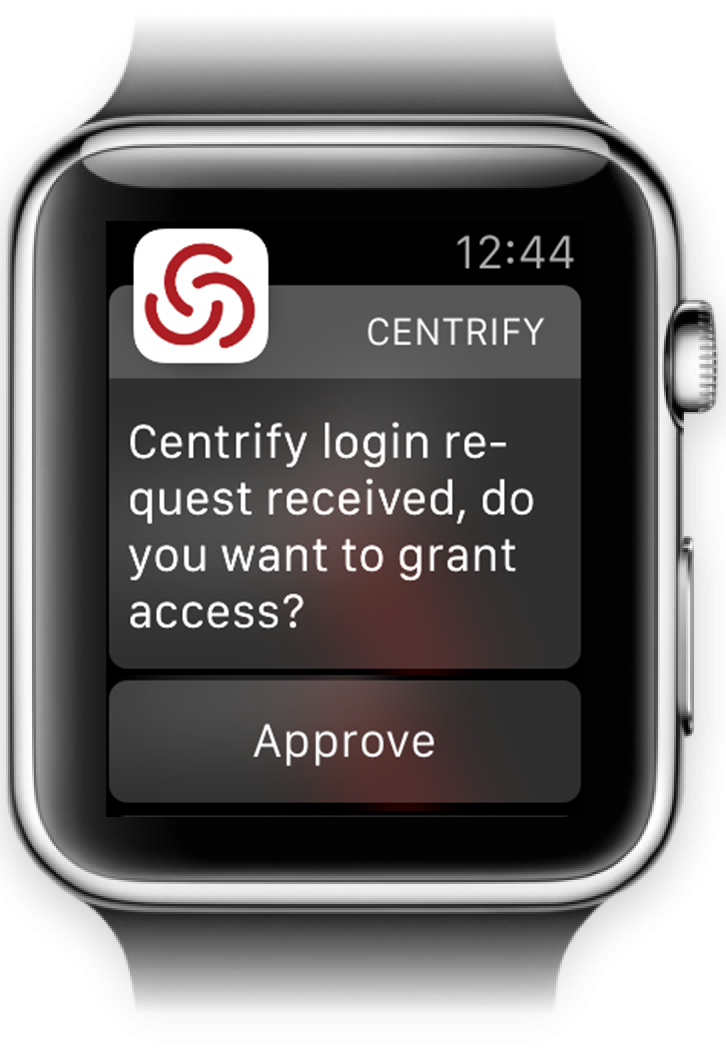
\includegraphics[width=.35\linewidth]{gfx/consent}
    \caption{Example of Explicit User Consent}
\end{figure}

\subsection{Why Wearables?}
\fquotet{A general trend is clear: wearables provide novel opportunities \\ to improve or re- design approaches to authentication.}{bianchi2016wearable}
\bigskip

\citet{ojala2008wearable} used an approach with wearable authentication in their proposed scheme. Their solution was a custom built wearable wristband with different sensors and a computer attached, which was highly specialized to be used for authentication only. 
Within recent years wearable computing devices (commonly referred to as 'wearables') has become available to the end-user market, intended for multi-purpose use, and not for authentication only. These recent advances have made wearables regain the attention from security researchers, to explore the different opportunities that wearables can provide for user authentication \cite{bianchi2016wearable}. 
We want our authentication scheme to utilize wearables, for several reasons. First, the many sensors embedded into wearables provide an easy way to harvest input data implicitly about the wearing user. Furthermore many wearable devices come with light sensors that can report when a user is wearing the device or have taken it off. In short, the embedded sensors can help to establish more confidence in a user's identity, which is very useful for providing secure authentication. Second, the processing power and network capabilities of wearables have grown, now enabling them to run authentication mechanisms based on strong cryptography. Third, the use of wearables allows our protocol to run on commodity hardware, that is already widely known and used, thus allowing us to focus less on hardware details of the scheme, and at the same time increasing the chance that users will adopt the system, if they already own the required hardware. 

\subsection{Proximity}
In order to provide transparent authentication, some mechanisms must be put in place to autonomously decide when and where authentication should take place, whenever the user is not directly involved in the process. Taking inspiration from both \citet{bardram2003context} and \citet{ojala2008wearable} we want the authentication scheme to be proximity-based. Ideally, a user should be able to walk up to a computer and as soon as he is within a specified range, the transparent authentication process should initiate. To do this a user must carry a wearable device that is capable of providing evidence of the user's identity, to client computers where the user wants to authenticate at. We imagine that the Bluetooth protocol would be an ideal solution to support proximity-based authentication between the wearable devices and the client computers. While it may be an implementation detail, Bluetooth is to a large extend the communication standard that what we have had in mind when we designed our scheme. Additionally, the choice of a widely used communication standard as Bluetooth also aligns well with our choice of wearables, and the preference of mature commodity technologies over highly specialized solutions.

\subsection{Continuity}

When making the authentication mechanism more transparent (unobtrusive), a problem might be that the user is not aware that he is authenticated with the system that he is using (even if the information is available to him, he might overlook the fact), and thus walk away from an active session. 

\fquotet{During our experiments we discovered that the process of logging out a user is equally important. [...] Although this is normally not considered to be part of a user authentication mechanism, we argue that logout has to be considered as a part of the design as well.}{bardram2003context}

Continuous authentication entails verification of user identity on an ongoing basis during an authentication session, thus greatly increasing the certainty that only the legitimate user is accessing protected resources~\cite{ojala2008wearable}. A problem with many services today, is that clients are allowed to store user credentials or save access tokens without expiration in cookies, such that no confirmation of the user's identity is done after initial verification. This design is needed to reduce constant user interaction, because of the heavy reliance of password in current schemes. However this comes with the trade-off, that a non legitimate user can access private resources, in case of theft or loss of a device. 

We found that continuous authentication synergises well with prox\-imity-based, transparent and wearable authentication. 
Since we are using a transparent authentication scheme we do not need to store login information on the client, since the information needed to verify a user's identity, can be acquired without interrupting the user, even if it is done very frequently. After a user has established initial authentication, we can continually confirm that the basic requirements for authentication are still met, such as the user having to wear the wearable device actively, and be within proximity of the client he is authenticated at.

It is important to mention that literature uses the term `continuous' differently. It can either describe the process of continuous verification to keep an authenticator unlocked (as in the case of the Pico~\cite{stajano2011pico}), or be a continuous verification process with a verifier (as in the case of Wearable Auth~\cite{ojala2008wearable}). We aim to include \textit{both} aspects.

\subsection{Authenticator and Sibling}
In order to make our scheme more resilient to theft or loss of the wearable device, and also less vulnerable in case the device is compromised, the scheme is designed to be used with an additional device, that works together with the wearable device to decide whether authentication is allowed or not. If an attacker gains access (physically or virtually), to one of the devices, but not both, it should not be possible to achieve any successful attacks. We have designed it such that the device pair, form a master/slave relationship, where outside parties communicate only with the master device to request authentication access. We generally refer to the two devices as the \gls{authenticator} acting as the master and the \gls{sibling} acting as the slave device. Loosely defined the \gls{authenticator} could be any type of computational device. Table~\ref{table:device_table} shows the requirements for the two devices. 

\begin{table}[bth]
\centering
\vspace{8em}
%\resizebox{\linewidth}{!}{
% \setlength\tabcolsep{1.8pt}
\begin{tabular}{r|ccccccc}
& \begin{rotate}{55}\textit{Being worn by a user}\end{rotate}
& \begin{rotate}{55}\textit{Verifying a users identity}\end{rotate}
& \begin{rotate}{55}\textit{Monitoring if worn}\end{rotate}
& \begin{rotate}{55}\textit{Receiving basic user-input}\end{rotate}
& \begin{rotate}{55}\textit{Displaying messages}\end{rotate}
& \begin{rotate}{55}\textit{Cryptographic computations}\end{rotate}
& \begin{rotate}{55}\textit{Bluetooth LTE I/O} \end{rotate} \\ \hline

Authenticator &
\CIRCLE &
\CIRCLE &
\CIRCLE &
\CIRCLE &
\CIRCLE &
\CIRCLE &
\CIRCLE \\ \hline
Sibling &
&
&
&
&
&
\CIRCLE &
\CIRCLE \\ \hline

    \end{tabular}
%}
\caption[Overview of device requirements]{The requirements of devices used as authenticators and siblings.}
\label{table:device_table}
\end{table}

\begin{comment}
\begin{itemize}
    \item Being worn by a user
    \item Verifying a users identity
    \item Monitoring when it is worn and when it is taken off
    \item Receiving basic input from user
    \item Displaying output messages
    \item Performing basic cryptographic computations 
    \item Sending/receiving data over Bluetooth
\end{itemize}

The \gls{sibling} has fewer requirements. It can be any type of computational device, as long as it is capable of:
  
\begin{itemize}
    \item Performing basic cryptographic computations 
    \item Sending/receiving data over Bluetooth
\end{itemize}
\end{comment}

While we claim that our scheme design and concepts of \gls{authenticator} and \gls{sibling} are not locked to a specific device type, we have primarily considered and worked with the case of a smartwatch as \gls{authenticator} and a smartphone as \gls{sibling}. We will therefore not rule out completely, that certain design choices have been made with these two device types in mind. The main reason for this is to use devices that the user will already carry around with him. Although wearables are not so common yet, they are slowly getting traction. By using devices that the user already has in his vicinity, we increase the transparency of the solution, both in terms of the user not needing to remember bringing a dedicated authentication device, and in terms of hiding the solution in devices, he already carries around.

%\todo[inline]{We need to change this part. The main argument should be that it is devices that the user (likely) already owns and carries around.}

%The reason for choosing a smartwatch and smartphone, is that in addition to each fulfilling all the basic requirements listed above, they are both easy to work and experiment with from a prototyping perspective. This has allowed us to focus on scheme design and core functionality, and not hardware/software issues related to the platform.
%Another benefit is that both device types are widely available and recognized as consumer products, which makes it more easy for readers of this thesis to relate to, and understand how they could be used in practice. 


\section{The Scheme in Practice} \label{sec:scheme_desc}
The design choices above, lead us to the following more brief and concrete description of how our authentication scheme should work in practice:

The scheme involves 4 different communicating parties. The \gls{authenticator}, the \gls{sibling}, the \gls{client} and the \gls{server}. A user carries two personal physical devices: the \gls{authenticator} and the \gls{sibling}, which are a smartwatch and a smartphone respectively. The \gls{authenticator} acts as a key which is unique to each user and required for authentication. However the \gls{authenticator} should only allow authentication if it is actively worn by the user, and in proximity of its \gls{sibling} device. If at any time the user takes off the \gls{authenticator} from his wrist, or if the \gls{sibling} is not nearby, the \gls{authenticator} should go into \textbf{locked} state, effectively meaning that all authentication requests it receives are denied. Furthermore, the \gls{authenticator} should return to \textbf{unlocked} state once the \gls{sibling} is again within proximity, or if the user re-equips the \gls{authenticator} on his wrist and reconfirms his identity, either by using biometric sensors, pin code or some other mechanism available from the \gls{authenticator}.  

The user interacts with a \gls{client} which is the device from where the authentication process is initiated. A \gls{client} could for instance be a laptop or desktop computer, which is used to login to some online service, that requires authentication. 

The \gls{client} is not an active participant in the authentication process. Rather, when the user tries to authenticate with a \gls{server} through the \gls{client}, and the \gls{authenticator} is nearby and \textbf{unlocked}, then the \gls{authenticator} will be required to provide evidence of the identity.
If the evidence is accepted by the \gls{server}, then the \gls{client} is authenticated.

%The \gls{client} is not directly handling authentication but merely contacts a \gls{server} that owns some protected resources. The \gls{server} requires the \gls{client} to prove that the \gls{authenticator} is indeed in range of the \gls{client} and is worn by the user, in order to allow access to its resources. Thus the main responsibility of the \gls{client} is to serve content, and act as a middle man for communication between the \gls{authenticator} and the \gls{server}.

The scheme is backed by a protocol that continually authenticates the user as long as the \gls{authenticator} is worn in close range of the \gls{client} and in \textbf{unlocked} state. If one of the conditions are not met at any time, the authentication session should terminate.

\begin{figure}
  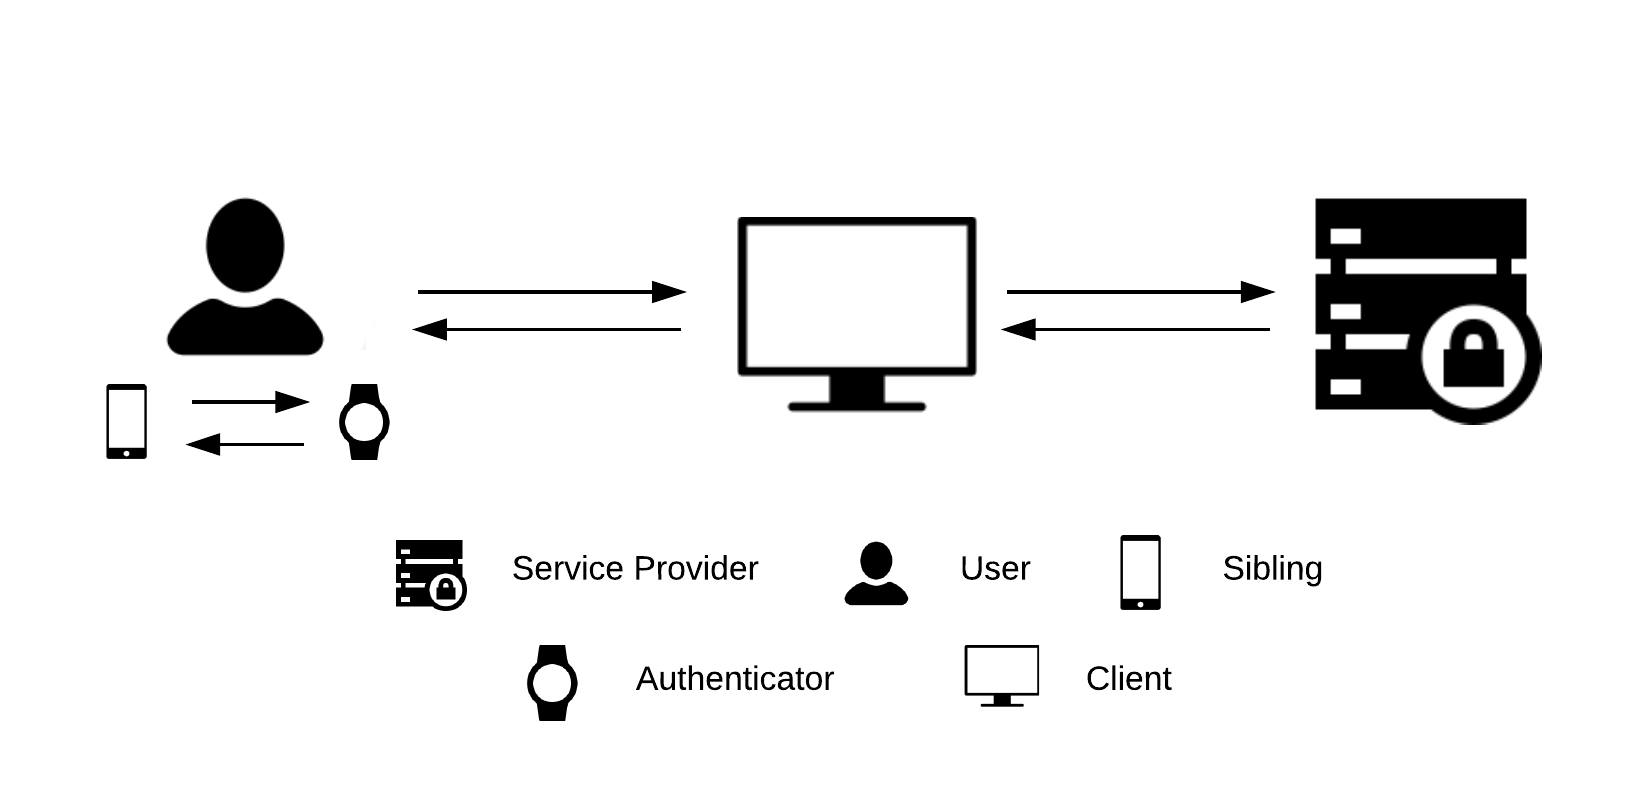
\includegraphics[width=\linewidth]{gfx/scheme_diagram.png}
  \caption{Component overview for the propose scheme}
  \label{fig:scheme_diagram}
\end{figure}


\section{User Scenarios} \label{sec:scenarios}
Below we describe 4 different user scenarios for our authentication scheme. The scenarios describe the most commonly occurring situations in the use of our proposed scheme. The intention of these scenarios is to gain insight into how the user interacts with the system, and to demonstrate which problems it solves for the user. 
The different actors appearing across the scenarios are the same as presented above in \ref{sec:scheme_desc}: \gls{authenticator}, \gls{sibling}, \gls{client} and \gls{server}. We differentiate between two levels of user involvement, where \gls{awareness} is the least obtrusive of the two:
\begin{itemize}
    \item[] \Gls{awareness}: \textit{The user is notified about important events, but does not require the user to actively perform any actions.}
    \item[] \Gls{exp_consent}: \textit{The user is required to actively perform an action, typically in the form of accepting/denying certain requests between the involved actors.}
\end{itemize}

The scenarios are listed in table~\ref{sc:register}, \ref{sc:unlocking}, \ref{sc:auth}, and \ref{sc:theft}.



\begin{scenario}{Registration with a Service Provider}{Scenario: Registration}{register}
    \row{Actors}{\gls{authenticator} $A$, \gls{client} $C$, \gls{server} $S$}
    \row{User involvement}{Awareness, optional:Explicit consent}
    \row{Authenticator State}{$unlocked$}
    \row{Description}{A user wants to register for a service $S$ and uses a \gls{client} $C$ to send a registration request to $S$. $S$ now communicates with the users \gls{authenticator} $A$ through $C$ and asks for confirmation of the registration. $A$ now notifies the user and optionally ask the user to confirm the registration request, before sending back needed information to $S$ to complete the registration process.}
\end{scenario}

\begin{scenario}{Unlocking the Authenticator}{Scenario: Unlocking}{unlocking}
    \row{Actors}{\gls{authenticator} $A$, \gls{sibling} $As$}
    \row{User involvement}{Awareness, optional:Explicit consent}
    \row{Authenticator State}{$locked \Rightarrow unlocked$}
    \row{Description}{A users watch acting as \gls{authenticator} $A$ is $locked$ and he wishes to unlock it. The user puts on the watch, which registers that it has been put on by its owner, and starts monitoring that it remains attached. $A$ now communicates with its sibling $As$, and asks for permission to unlock. After an optional user interaction with $As$, it communicates back with an acknowledgement, that allows $A$ to unlock. $A$ now notifies the user that it is $unlocked$. $A$ remains $unlocked$ for as long it is attached to the users wrist, and in range of $As$.}
\end{scenario}

\begin{scenario}{Establishing a Session}{Scenario: Authentication}{auth}
    \row{Actors}{\gls{authenticator} $A$, \gls{client} $C$, \gls{server} $S$}
    \row{User involvement}{Awareness, optional:Explicit consent}
    \row{Authenticator State}{$unlocked$}
    \row{Description}{A user wants to establish a session with a \gls{server} $S$ through a \gls{client} $C$. $S$ replies with a challenge, which requires $C$ to prove that it is a legitimate user who is requesting access. $C$ forwards the challenge to the users nearby \gls{authenticator} $A$, which is currently $unlocked$. $A$ optionally asks the user to confirm the authentication request, and then replies back with a response to the challenge generated by $S$. $C$ now sends the challenge response back to $S$, and if $S$ accepts the solution to the challenge, then an authentication sessions is established. $A$ notifies the user that the sessions is established. If the session is not explicitly cancelled by the user, the session is maintained as long as $A$ remains unlocked and $A$ remains in proximity of $C$.}
\end{scenario}

\begin{scenario}{Theft or Loss}{Scenario: Theft or loss}{theft}
    \row{Actors}{\gls{authenticator} $A$, \gls{sibling} $As$}
    \row{User involvement}{Explicit consent}
    \row{Authenticator State}{$unlocked \lor locked \Rightarrow lockdown$}
    \row{Description}{A user notices that either his \gls{authenticator} $A$ or \gls{sibling} $As$ is missing. The user uses the remaining device to activate $lockdown$. In this state $A$ can no longer be unlocked (even when in proximity of $As$), and therefore not authenticate with any services. The $lockdown$ state remains until a recovery procedure has taken place, either if the missing device resurfaces, or if a new device is used for recovery.}
\end{scenario}


\section{Scheme Evaluation}

In this section we evaluate our proposed authentication scheme, in comparison to the review in chapter~\ref{ch:review}. In addition to the benefits defined by the framework, we define four new properties, that we based on our analysis consider equally relevant for authentication. An overview is shown in table~\ref{table:property_table}.



\subsection{Extending the Evaluation Framework}\label{sec:extending_framework}
We extend the framework \cite{bonneau2012quest}, with 2 usability properties: \textit{Awareness} and \textit{No-Config}; and 2 security properties: \textit{No-Intermediary-Knowledge} and \textit{Continuous}. 

\paragraph{Awareness:} The scheme can make its users aware of its current state, and the decisions it takes autonomously. We grant \textit{Awareness} if a user of the scheme is capable of knowing where he is currently authenticating/authenticated at, at all times. This benefit is considered important from a usability perspective, since it helps a user to understand what happens transparently, and avoid undesirable situations as where a user think he is authenticated but actually is not, and conversely actually is authenticated, but think he is not.
    
\paragraph{No-Config:} We award \textit{No-Config} if the act of authentication or user registration does not require any additional configuration steps the first time a specific client is used by a specific user, compared to if the client was used previously by the specific user. 
Thus a user must be able to walk up to any arbitrary client and use the scheme for authentication or registration, with the same amount of required effort, as on a client where he has used the scheme, several times before. Note that \textit{No-Config} does not mean that no initial configuration might be needed on a client in order to run the scheme (eg. installing a browser plugin or enabling Bluetooth). Rather it means that no additional configuration is required specifically because it is a new user of the client. Password managers are a type of scheme that typically does not offer this benefit, since a user will have to undergo an extra step the first time he uses a new client in order to transfer his keychain onto it. The benefit of \textit{No-Config} is considered a usability benefit, because it reduces the time a user has to spend on authentication the first time he uses a new client. It is especially important in environments where many public computers are used, and a user does not have a personal computer.
    
\paragraph{No-Intermediary-Knowledge:} During authentication or registration the client is not exposed to any information with long-term value. We grant \textit{No-Intermediary-Knowledge} if no secrets (such as passwords), that could be used to authenticate at a later point in time, is given or inputted on the client. \textit{No-Intermediary-Knowledge} is a security benefit and is considered important because it limits the power of an adversary in full or partial control of the client.
    
\paragraph{Continuous:} The scheme supports continuous authentication. We grant the benefit if a scheme reconfirms a user's identity with a verifier regularly after initial authentication, and is capable of stopping the authentication session whenever the user's identity can not be verified any longer. This benefit is a security benefit, and limits the power of an adversary with physical or remote access to a client greatly, since the authentication sessions are not kept alive for an extended duration after the user is no longer actively engaged.

We grant \textit{Quasi-Continuous} if the system is using a hardware token and only the token is continuously authenticated, but sessions with services are not.

\subsection{Rating Process} \label{sec:rating_process}
The authentication scheme proposed in this thesis is intended as an improvement over password. It aims to improve security and usability of passwords, but does not aim to surpass passwords in terms of deployability.

The scheme is \textit{Memorywise-Effortless} by design because it is a transparent authentication scheme, and therefore does not require the user to input anything from memory or perform some memorized interaction in order to authenticate. For the same reasons and since no new hardware has to be introduced to the user, we award \textit{Easy-to-learn}. The proximity-based login approach of the scheme ensures that it is \textit{Physically-Effortless} to use, as the only real physical requirements of the user to use the scheme for authentication, is that the user must wear a watch and carry a phone, and move within close range of the client where authentication is performed at. 

We grant \textit{Efficient-to-Use} and \textit{Infrequent-Errors} because the scheme is designed to have minor user interaction, and the cryptographic exchanges between \gls{server} and \gls{authenticator}, is carried out much faster than the time taken for typing even a simple password. Furthermore, the scheme does not rely on biometrics or other methods of authentication that could introduce false-negatives. The scheme is \textit{Scalable-for-Users}, as an increased number of links between users and \glspl{server} does not have any impact on the individual users experience. We award the scheme \textit{Quasi-Nothing-to-Carry}, because the benefit can only be granted if the user has to carry nothing at all. However, if the devices are considered something which the user always carry around anyway, in this case, a phone and a watch, the applied burden on the user is arguably reduced significantly. We do not grant the scheme \textit{Easy-Recovery-from-Loss} since no such mechanism exists for the scheme in its current design state. 
We grant \textit{Awareness} as the scheme is designed to send notifications to a user on his watch, whenever a new registration or authentication session is started. The scheme does not offer the benefit of \textit{No-Config} as a pairing process is required between \gls{client} and \gls{authenticator}, the first time a new \gls{client} is used. 

\begin{table}[bth]
\centering
\begin{wide}
\resizebox{\linewidth}{!}{
%\rotatebox{270}{
\setlength\tabcolsep{1.8pt}
\begin{tabular}{r|c|cccccccccc|cccccc|ccccccccccccc}

\multicolumn{2}{c}{} &
\multicolumn{10}{c}{\textbf{Usability}} &
\multicolumn{6}{c}{\textbf{Deployability}} &
\multicolumn{13}{c}{\textbf{Security}}\\
\multicolumn{31}{c}{}
\\

& \rot{\textit{Reference}} &
\rot{\textit{Memorywise-Effortless}} &
\rot{\textit{Scalable-for-Users}} &
\rot{\textit{Nothing-to-Carry}} &
\rot{\textit{Physically-Effortless}} &
\rot{\textit{Easy-to-Learn}} &
\rot{\textit{Efficient-to-Use}} &
\rot{\textit{Infrequent-Errors}} &
\rot{\textit{Easy-Recovery-from-Loss}} &
\rot{\textit{Awareness}} &
% \rot{\textit{Multi-User-Support}} &
\rot{\textit{No-Config}} &
\rot{\textit{Accessible}} &
\rot{\textit{Negligible-Cost-per-User}} &
\rot{\textit{Server-Compatible}} &
\rot{\textit{Browser-Compatible}} &
\rot{\textit{Mature}} &
\rot{\textit{Non-Proprietary}} &
\rot{\textit{Resilient-to-Physical-Observation}} &
\rot{\textit{Resilient-to-Targeted-Impersonation}} &
\rot{\textit{Resilient-to-Throttled-Guessing}} &
\rot{\textit{Resilient-to-Unthrottled-Guessing}} &
\rot{\textit{Resilient-to-Internal-Observation}} &
\rot{\textit{Resilient-to-Leaks-from-Other-Verifiers}} &
\rot{\textit{Resilient-to-Phishing}} &
\rot{\textit{Resilient-to-Theft}} &
\rot{\textit{No-Trusted-Third-Party}} &
\rot{\textit{Requiring-Explicit-Consent}} &
\rot{\textit{Unlinkable}} &
\rot{\textit{No-Intermediary-Knowledge}} &
\rot{\textit{Continuous}} \\ \hline

Passwords & &
            & %Memorywise-Effortless
            & %Scalable-for-Users
\CIRCLE     & %Nothing-to-Carry
            & %Physically-Effortless
\CIRCLE     & %Easy-to-Learn
\CIRCLE     & %Efficient-to-Use
\Circle     & %Infrequent-Errors
\CIRCLE     & %Easy-Recovery-from-Loss
            & %Awareness
%           & %Multi-User-Support
\CIRCLE     & %No-Pairing
\CIRCLE     & %Accessible
\CIRCLE     & %Neglible-Cost-per-User
\CIRCLE     & %Server-Compatible
\CIRCLE     & %Browser-Compatible
\CIRCLE     & %Mature
\CIRCLE     & %Non-Proprietary
            & %Resilient-to-Physical-Observation
\Circle     & %Resilient-to-Targeted-Impersonation
            & %Resilient-to-Throttled-Guessing
            & %Resilient-to-Unthrottled-Guessing
            & %Resilient-to-Internal-Observation
            & %Resilient-to-Leaks-from-Other-Verifiers
            & %Resilient-to-Phishing
\CIRCLE     & %Resilient-to-Theft
\CIRCLE     & %No-Trusted-Third-Party
\CIRCLE     & %Requiring-Explicit-Consent
\CIRCLE     & %Unlinkable
            & %No-Intermediary-Knowledge
              %Continuous
\\ \hline

Context-Aware Auth~~& \cite{bardram2003context} &
\Circle     & %Memorywise-Effortless
\CIRCLE     & %Scalable-for-Users
            & %Nothing-to-Carry
\Circle     & %Physically-Effortless
\CIRCLE     & %Easy-to-Learn
\CIRCLE     & %Efficient-to-Use
\CIRCLE     & %Infrequent-Errors
            & %Easy-Recovery-from-Loss
            & %Awareness
%           & %Multi-User-Support
\CIRCLE     & %No-Pairing
\CIRCLE     & %Accessible
            & %Neglible-Cost-per-User
            & %Server-Compatible
            & %Browser-Compatible
            & %Mature
\CIRCLE     & %Non-Proprietary
\Circle     & %Resilient-to-Physical-Observation
\CIRCLE     & %Resilient-to-Targeted-Impersonation
            & %Resilient-to-Throttled-Guessing
            & %Resilient-to-Unthrottled-Guessing
\Circle     & %Resilient-to-Internal-Observation
            & %Resilient-to-Leaks-from-Other-Verifiers
\Circle     & %Resilient-to-Phishing
\Circle     & %Resilient-to-Theft
            & %No-Trusted-Third-Party
\CIRCLE     & %Requiring-Explicit-Consent
            & %Unlinkable
\Circle     & %No-Intermediary-Knowledge
\Circle       %Continuous
\\ \hline

Wearable Auth & \cite{ojala2008wearable} &
\CIRCLE     & %Memorywise-Effortless
\CIRCLE     & %Scalable-for-Users
\Circle     & %Nothing-to-Carry
\Circle     & %Physically-Effortless
\CIRCLE     & %Easy-to-Learn
\CIRCLE     & %Efficient-to-Use
\CIRCLE     & %Infrequent-Errors
            & %Easy-Recovery-from-Loss
            & %Awareness
%           & %Multi-User-Support
            & %No-Pairing
\CIRCLE     & %Accessible
            & %Neglible-Cost-per-User
            & %Server-Compatible
            & %Browser-Compatible
            & %Mature
\CIRCLE     & %Non-Proprietary
\CIRCLE     & %Resilient-to-Physical-Observation
\CIRCLE     & %Resilient-to-Targeted-Impersonation
\CIRCLE     & %Resilient-to-Throttled-Guessing
\CIRCLE     & %Resilient-to-Unthrottled-Guessing
?           & %Resilient-to-Internal-Observation
?           & %Resilient-to-Leaks-from-Other-Verifiers
\CIRCLE     & %Resilient-to-Phishing
\CIRCLE     & %Resilient-to-Theft
?           & %No-Trusted-Third-Party
\Circle     & %Requiring-Explicit-Consent
?           & %Unlinkable
?           & %No-Intermediary-Knowledge
\CIRCLE       %Continuous
\\ \hline

Pico & \cite{stajano2011pico} &
\CIRCLE     & %Memorywise-Effortless
\CIRCLE     & %Scalable-for-Users
            & %Nothing-to-Carry
\CIRCLE     & %Physically-Effortless
            & %Easy-to-Learn
\Circle     & %Efficient-to-Use
\Circle     & %Infrequent-Errors
            & %Easy-Recovery-from-Loss
            & %Awareness
%           & %Multi-User-Support
            & %No-Pairing
            & %Accessible
            & %Neglible-Cost-per-User
            & %Server-Compatible
            & %Browser-Compatible
            & %Mature
\CIRCLE     & %Non-Proprietary
\CIRCLE     & %Resilient-to-Physical-Observation
\CIRCLE     & %Resilient-to-Targeted-Impersonation
\CIRCLE     & %Resilient-to-Throttled-Guessing
\CIRCLE     & %Resilient-to-Unthrottled-Guessing
\CIRCLE     & %Resilient-to-Internal-Observation
\CIRCLE     & %Resilient-to-Leaks-from-Other-Verifiers
\CIRCLE     & %Resilient-to-Phishing
\Circle     & %Resilient-to-Theft
\CIRCLE     & %No-Trusted-Third-Party
\CIRCLE     & %Requiring-Explicit-Consent
\CIRCLE     & %Unlinkable
\CIRCLE     & %No-Intermediary-Knowledge
\Circle       %Continuous
\\ \hline

Our design & &
\CIRCLE     & %Memorywise-Effortless
\CIRCLE     & %Scalable-for-Users
\Circle     & %Nothing-to-Carry
\CIRCLE     & %Physically-Effortless
\CIRCLE     & %Easy-to-Learn
\CIRCLE     & %Efficient-to-Use
\CIRCLE     & %Infrequent-Errors
            & %Easy-Recovery-from-Loss
\CIRCLE     & %Awareness
%           & %Multi-User-Support
            & %No-Pairing
\CIRCLE     & %Accessible
\Circle     & %Neglible-Cost-per-User
            & %Server-Compatible
            & %Browser-Compatible
            & %Mature
\CIRCLE     & %Non-Proprietary
\CIRCLE     & %Resilient-to-Physical-Observation
\CIRCLE     & %Resilient-to-Targeted-Impersonation
\CIRCLE     & %Resilient-to-Throttled-Guessing
\CIRCLE     & %Resilient-to-Unthrottled-Guessing
\Circle     & %Resilient-to-Internal-Observation
\CIRCLE     & %Resilient-to-Leaks-from-Other-Verifiers
\CIRCLE     & %Resilient-to-Phishing
\Circle     & %Resilient-to-Theft
\CIRCLE     & %No-Trusted-Third-Party
\Circle     & %Requiring-Explicit-Consent
\CIRCLE     & %Unlinkable
\CIRCLE     & %No-Intermediary-Knowledge
\CIRCLE       %Continuous
\\ \hline
\multicolumn{31}{r}{

\CIRCLE~=~offers the benefit 
\quad \Circle~=~almost offers the benefit
%\quad \textit{no circle}~=~does not offer the benefit 
\quad ?~=~not known}
\quad \\

\end{tabular}}
\end{wide}

\caption[Overview of benefits of our design]{Comparing the benefits of passwords with related work in Pervasive Authentication and the (envisioned) benefits of our design.}
\label{table:property_table}
\end{table}

The scheme is \textit{Accessible} since no physically constraining activities are involved in the use of the scheme. We grant it \textit{Quasi-Negligible-Cost-per-User}, as the required devices: smartphone and smartwatch, are relatively costly on one hand, but on the other hand is something that can be used for many other purposes and is already owned by many users.
As the scheme aims to be a complete password replacement, it is not designed to prioritize \textit{Server-Compatible} or \textit{Browser-Compatible}. We can therefore not award either benefit, as a whole new infrastructure is most likely needed by the service providers and verifies end. The scheme is \textit{Non-Proprietary}, but it is not \textit{Mature}.

A strong cryptographic protocol is used for the scheme, which in combination with the transparent proximity-based login mechanism ensures full ratings on most of the security benefits. We grant \textit{Resilient-to-Physical-Observation}, \textit{Resilient-to-Targeted-Impersonation}, simply because the scheme never requires users to reveal any information, in order to authenticate. The protocol used for the scheme requires a new cryptographic key pair to be used for each association between verifier and user, and thus offers the benefits \textit{Resilient-to-Leaks-from-Other-Verifiers} and \textit{Unlinkable}. The scheme also has \textit{No-Trusted-Third-Party}. We award \textit{Resilient-to-Throttled-Guessing} and \textit{Resi\-lient-to-Unthrottled-Guessing} as the protocol is based on El-Gamal encryption with a sufficiently large key space, to be practically impossible to guess even with large amounts of computing power. The protocol uses a challenge-response architecture, meaning that the only way to authenticate is to respond to a challenge that can only be solved by possessing the right secret key. The protocol never transmits or reveals any secrets keys, and thus no information can be acquired that can be used at a later point of time to authenticate. We therefore grant both \textit{No-Intermediary-Knowledge} and \textit{Resilient-to-Phishing}. The scheme aims for the \gls{authenticator} to continuously verify the presence of the user wearing the device, and to terminate any active sessions if the devices lock.  Thus we grant the benefit \textit{Continuous}.

While the scheme is designed to offer many of the security benefits, it has a few weak points where we can only award `quasi' rating. The scheme is \textit{Quasi-Resilient-to-Theft} as it is not enough to steal the watch without the phone and vice versa. Furthermore, the watch can be pin-code protected if it gets stolen, although it is a rather weak form of protection. Since the scheme relies on smartphones and smartwatches, and not a dedicated hardware device, we must assume that it is a possibility that malware exists on either device which can potentially be harmful to the execution of the scheme. However it is only harmful in case both devices are malware infected, and thus we grant \textit{Quasi-Resilient-to-Internal-Observation}.

The scheme can by design not offer the benefit \textit{Requiring-Explicit-Consent} fully, as parts of the authentication process are done transparently. However, the scheme defines an option for adding explicit user consent in certain situations, by prompting users for confirmation of new authentication sessions and registrations. 



\subsection{Extending the Review}\label{sec:results_overview}

To compare the previously considered schemes, we extend their review to include the new benefits.

None of the previously considered mechanisms are granted \textit{Awareness}. Passwords, Context-Aware Auth and Pico are granted \textit{No-Config}. Passwords obviously gain this benefit as using the scheme (assuming that user always has to log in when using a service) is the same for all clients. Similarly, for Context-Aware Auth, the login process is the same for all supporting clients. Pico uses a two-channel communication approach. One channel is a visual channel. When the user wishes to authenticate, the Pico is used to scan a QR-code on the screen. The Pico then opens a communication channel to the service and authenticates the user. Therefore no configuration is needed when using a new client.

We grant \textit{No-Intermediary-Knowledge} to Pico as the utilized client is not given any pertinent information except for a temporary authentication token. Context-Aware auth is granted \textit{Quasi-No-Intermediary-Knowledge}, as the user might occasionally input his password on the client.

Wearable Auth is granted \textit{Continues}, as the wearable locks if not actively worn. Furthermore, the wearable must be present near the client or the client will lock. Pico is granted \textit{Quasi-Continuous} as the Pico continuously verifies the presence of its siblings, but does (seemingly) not terminate active sessions with services if locked. Context-Aware Auth is granted \textit{Quasi-Continuous} as a user can walk away from an active session if he forgets his keycard in the machine. The system is not described to terminate the session if the context service no longer registers the user at the client.


%*****************************************
%*****************************************
%*****************************************
%*****************************************
%*****************************************

%************************************************
\chapter{Protocol Design}\label{ch:protocol}
%************************************************


% What is the goals of an adversary?
% - Be able to forge authentication
% - Be able to link different identities to the same user.
% - Be able to use/hijack an active session


In the previous chapter, we present a design for a \gls{cta} authentication scheme. In this chapter we will present a protocol, which is simply a sequence of well-chosen messages, that can support this scheme. In this chapter, we will only highlight a few important properties from the previous chapter in regards to certain choices, and will then later evaluate which properties the proposed protocol achieves.

\section{Definition of Authentication}

So far we have not clearly defined what `authentication' actually entails. In his well-renowned article ``A Hierarchy of Authentication Specifications'' \citet{lowe1997hierarchy} puts forward the following definition:

\begin{definition}[Injective Agreement]
We say that a protocol guarantees to an initiator $A$ agreement with a responder $B$ on a set of data items $ds$ if, whenever $A$ (acting as initiator) completes a run of the protocol, apparently with responder $B$ , then $B$ has previously been running the protocol, apparently with $A$, and $B$ was acting as responder in his run, and the two agents agreed on the data values corresponding to all the variables in $ds$, and each such run of $A$ corresponds to a unique run of $B$.
\end{definition}

This definition infer that if two parties agree on a set of data (or evidence of identity), and if there is a one-to-one relationship between the protocol run at the responder and verifier, then they achieve (injective) agreement, and thus the responder authenticates with the verifier.

\section{Design Rationale}
Our design inspires from this definition, and effectively, the \gls{server} $S$, will on request from the \gls{client} $C$, issue a fresh challenge. If the client can reply with a proper response to the challenge then it should be authenticated for a given period of time. Let us consider a simple example in which the \gls{server} encrypts a random nonce with the public-key of the \gls{client}, and sends the cipher to the client. The client then decrypts the cipher and responds to the challenge with the recovered nonce.
{\setlength{\mathindent}{0cm}
\begin{align}
    \tag{message 1} && S \rightarrow C &: enc(n,pk_c)\\
    \tag{message 2} && C \rightarrow S &: n
\end{align}}

Only an actor in possession of $sk_c$ would be able to recover the correct answer, and thus presenting $n$, serves as evidence of knowing $sk_c$. This can be used to authenticate if the server links the public key to a user-identity. This will serve as a starting point for this protocol. However, a few design features from the previous chapter needs to be considered:
\begin{itemize}
    \item The \gls{client} should ask the \gls{authenticator} for `permission' to authenticate.
    \item The \gls{authenticator} should only give permission if unlocked; thus in range of the \gls{sibling}.
    \item The \gls{client} should not be exposed to any piece of information that could be used in a later successful round of authentication. 
    \item  Hijacking an active session or token should not give an \gls{adversary} unauthorized access for longer than the session is actively kept alive by the \gls{server} and \gls{authenticator}.
\end{itemize}

In the design, we mention that the \gls{authenticator} can be in a state of either unlocked, locked or lockdown. In practice, we take a different approach to implementing these states. As we envision using general-purpose commodity platforms such as e.g. iOS and Android devices, compromised devices are a concern that should be inherently designed for, and solely trusting a single device to uphold these states is therefore not an option.

\subsection{Distributed Authentication}


To ensure that \gls{authenticator} and \gls{sibling} are always involved in an authentication run, the unlocked state will in practice be implemented by forcing the \gls{authenticator} and \gls{sibling} to collaborate, in computing the response to an authentication challenge. If communication between \gls{authenticator}, \gls{sibling} and \gls{client} are forced onto a local channel (such as Bluetooth), then authentication is only possible when all three devices are in each others proximity.\\

In comparison, Pico~\cite{stajano2011pico} functions by having a main device, the Pico, that is the users key-store. The key-store is encrypted with a \textit{$k$-out-of-$n$} threshold encryption system. This means that at least $k$ siblings (small wearable tokens) must be in its vicinity for it to unlock. On request from the Pico, the siblings send their key-share, allowing the Pico to unlock its key-store. An assumption is made on the Pico, that it periodically `forgets' the key, thus forcing it to continuously interact with its siblings.

We see this as a problem because if the Pico is compromised in the unlocked state, then \textit{all} of the user's services are compromised. In the original paper, it is assumed that an adversary is not capable of compromising the Pico in the unlocked state. This is an unrealistic assumption when using general-purpose devices.

The rationale behind having a central unit holding all keys, and having peripheral devices unlocking, instead of having all devices actively participate, was taken with consideration to the technical limitations of wearables~\cite{stannard2012good}. However, since the Pico was proposed in 2011, these limitations are diminishing, and modern wearables are now fully capable of making cryptographic calculations without draining their battery.\\

The collaboration between \gls{authenticator} and \gls{sibling} can be achieved with `secure multiparty computations' (MPC). MPC entails a group of agents jointly computing a function, such as decrypting a cipher, without revealing anything about their individual input to the function. Furthermore, only with full participation from all actors will the output of the function be meaningful. This means that both devices would have to be compromised, for an adversary to be able to obtain the secrets needed to compromise the user's services. In practice, MPC can be implemented by utilizing a partial crypto system.\\





\begin{comment}
\paragraph{Security Goals}
\begin{itemize}

    \item An adversary should not be able to forge evidence of identity without compromising the secrets of both \gls{authenticator} and \gls{sibling}.
    
    \item Hijacking an active session or token should not give the \gls{adversary} unauthorized access for longer than the session is actively kept alive by the \gls{server} and \gls{authenticator}.
    
\end{itemize}
\end{comment}

\section{Partial Crypto Systems}

A partial crypto systems is a system in which multiple actors have to collaborate to encrypt and decrypt messages. Such systems are useful because they ensure that even if one of the actors is compromised, then the system is not compromised. Many such systems exists, but in this section we will present Distributed ElGamal, which is a partial crypto system~\cite{brandt2005efficient}.


\paragraph{ElGamal Crypto System}

ElGamal is a probabilistic and homomorphic public-key crypto system based on the Diffie-Hellman assumption. ElGamal is secure against \Glspl{cpa} (\acrshort{cpa}), if the Decisional Diffie–Hellman (DDH) problem is hard~\cite[page 400]{katz2014introduction}.

Using the cyclic prime order groups, as defined in section~\ref{par:cyclic}, we can define ElGamal in the following way:

\begin{itemize}
    \item \textbf{Gen:} on input $1^n$ run $\mathcal{G}(1^n)$ to obtain a cyclic group $\langle \mathbb{G},q,g \rangle$. Then choose a uniform $x \in \mathbb{Z}_q$ and compute $y := g^x$. Then output the public-key $\langle \mathbb{G},q,g,y \rangle$ and the private-key $\langle \mathbb{G},q,g,x \rangle$
    
    \item \textbf{Enc:} on input of a public-key and a message $m \in \mathbb{G}$, choose a uniform $r \in \mathbb{Z}_q$ and output the ciphertext $c := ( my^r, g^r )$.
    
    %\begin{align*}
    %    && \langle m\cdot y^r, g^r \rangle
    %\end{align*}
    
    \item \textbf{Dec:} on input of a private-key and a ciphertext $c = ( \alpha, \beta )$, output the message $m := \alpha / \beta^x$.
    
    %\begin{align*}
    %    && m := \alpha / \beta^x
    %\end{align*}
\end{itemize}

\paragraph{Distributed ElGamal}\label{sec:deg}

The distributed variant of ElGamal leverages that the original crypto system is homomorphic. Although the system is homomorphic over both message and keys for both encryption and descryption, the following is focused on homomorphism over the keys for decryption\footnote{For some set of operators `$+$' and `$\times$'}. 
{\setlength{\mathindent}{0cm}
\begin{align*}
&&    Dec(c,sk_1) \times Dec(c,sk_2) = Dec(c,sk_1 + sk_2)
\end{align*}}\vspace{-1em}

Let each participating actor $i$ in the distributed system generate an ElGamal key-pair $( pk_i, sk_i )$, using the same cyclic group $\langle \mathbb{G}, q, g \rangle$, by choosing an uniform $x_i \in \mathbb{Z}_q$ and calculating $y_i = g^{x_i}$~\cite{brandt2005efficient}. The joint public and private-key is now given as: 
{\setlength{\mathindent}{0cm}
\begin{align*}
&& y = \prod^n_{i=1} y_i && x = \sum^n_{i=1} x_i
\end{align*}}

An encrypted message $Enc(m,pk) \rightarrow ( \alpha, \beta )$ can be jointly decrypted by each participant calculating $\beta^{x_i}$. The message can then be recovered as:
{\setlength{\mathindent}{0cm}
\begin{align*}
&&    m := \frac{\alpha}{\prod^n_{i=1} \beta^{x_i}} = \frac{\alpha}{\beta^{x}}
\end{align*}}

The advantage of this is that the computation and sharing of $\beta^{x_i}$, following the DDH assumption, does not leak any information about the private-keys. Neither does the shares leak any information about the encrypted message before all shares are combined. We define the new operations as:
\begin{itemize}

    \item \textbf{Gen':} on input of a cyclic group $\langle \mathbb{G}, q, g \rangle$, choose a uniform $x \in \mathbb{Z}_q$ and calculate $y = g^{x}$. Then output the public-key $\langle \mathbb{G},q,g,y \rangle$ and the private-key $\langle \mathbb{G},q,g,x \rangle$

    \item \textbf{Dec':} on input of a private-key and a ciphertext $c = ( \alpha, \beta )$, output the partial decryption $c' := ( \alpha, \beta^{x_i} )$
    
    \item \textbf{Combine:} on input of two partially decrypted ciphertexts $c'_1 = ( \alpha, \beta^{x_1} )$ and $c'_2 = ( \alpha, \beta^{x_2} )$\marginpar{notice that the $\alpha$'s must match}, output
    {\setlength{\mathindent}{0cm} 
    \begin{align*}
    && c' := \left( \alpha, \beta^{x_1} \cdot \beta^{x_2} \right) = \left( \alpha, \beta^{{x_1}+{x_2}} \right)
    \end{align*}}\vspace{-2em}
    
    \item \textbf{Recover:} on input of a partially decrypted ciphertext $c' = ( \alpha, \beta^x )$, output the message $m := \alpha / \beta^x$
    
\end{itemize}

We denote the recovery of a message from combining partially decrypted ciphers as $m := Dec'(\cdot) \times Dec'(\cdot)$. Furthermore, we denote the product of public-keys as $pk := pk_1 \times pk_2$.

\section{The Protocol}

Two steps of the protocol has to be defined. A \gls{registration} and \gls{authentication} step. The purpose of the registration step is to establish a set of shared knowledge. The purpose of the authentication step is to provide the \gls{server} with evidence, and for the \gls{server} to be able to verify the authenticity of the evidence based on the knowledge acquired during the registration. The proposed protocol builds on the Distributed ElGamal crypto system as presented in the previous section.


\subsection{Registration}

The registration is initiated by the \gls{client} (and thus the end-user) by sending a message to the \gls{authenticator} with a universally unique user-id (such as a uuid\footnote{See \url{https://en.wikipedia.org/wiki/Universally_unique_identifier}}). The \gls{client} might have asked the \gls{server} in advance to issue this id based on some data such as a username. The \gls{authenticator} then forwards the message to the \gls{sibling} and starts computing a new Distributed ElGamal key-pair. The \gls{sibling} also computes a new Distributed ElGamal key-pair and sends its public-key to the \gls{authenticator}. The \gls{authenticator} now combines the keys to a joint public-key and sends it back to the \gls{client}. Lastly the \gls{client} sends the new public-key to the server along with the user-id. This is shown in figure~\ref{msc:register}.

\begin{figure}[bth]
\centering
\resizebox{\linewidth}{!}{
\begin{msc}{Registration}

\setlength{\instdist}{1.5cm}
\setlength{\actionwidth}{3cm}

\declinst{as}{}{$As$} 
\declinst{a}{}{$A$} 
\declinst{c}{}{$C$}
\declinst{s}{}{$S$} 

\nextlevel
\mess{$username$}{c}{s}
\nextlevel[2]
\mess{$id$}{s}{c}
\nextlevel
\mess{$id$}{c}{a}
\nextlevel
\mess{$id$}{a}{as}
\nextlevel
\action{Generate $( pk_{A}, sk_{A} )$}{a}
\action{Generate $( pk_{As}, sk_{As} )$}{as}
\nextlevel[4]
\mess{$pk_{As}$}{as}{a}
\nextlevel
\action{$pk = pk_A \times pk_{As}$}{a}
\nextlevel[4]
\mess{$id, pk$}{a}{c}
\nextlevel
\mess{$id, pk$}{c}{s}
\nextlevel

\end{msc}}
\caption[Registration sequence diagram]{The sequence of messages involved in a successful registration.}
\label{msc:register}
\end{figure}

\subsection{Authentication}
Authentication is initiated by the \gls{client} by sending an authentication request with a user-id to the \gls{server}. The \gls{server} responds with a challenge $c \leftarrow enc(n,pk)$, where $pk$ is the public-key corresponding to the user-id, and $n$ is an arbitrary nonce in $\mathbb{G}$. After sending the challenge the \gls{server} starts a timer $T$. The challenge is forwarded to the \gls{authenticator} and \gls{sibling} which both partly decrypts the challenge. The \gls{sibling} sends its partial decryption to the \gls{authenticator} which combines and recovers the nonce and sends it back to the \gls{server}. If the received nonce is correct then the \gls{server} issues a token to the client, valid for a given duration (in regards to the timer T). Before the token expires, the process is repeated to continuously keep the session active. This is shown in figure~\ref{msc:auth}.

\begin{figure}[bh]
\centering
\resizebox{\linewidth}{!}{
\begin{msc}{Authentication}

\setlength{\instdist}{1.5cm}
\setlength{\actionwidth}{3cm}

\declinst{as}{$\left(sk_{As}\right)$}{$As$} 
\declinst{a}{$\left(sk_{A}\right)$}{$A$} 
\declinst{c}{}{$C$}
\declinst{s}{$\left(pk\right)$}{$S$} 

\nextlevel
\mess{$id$}{c}{s}
\nextlevel
\inlinestart[1.75cm][1.75cm]{exp1}{loop}{as}{s}
\nextlevel
\action{$c \leftarrow enc(n,pk)$}{s}
\nextlevel[3]
\settimer[r]{T}{s}
\nextlevel
\mess{$c$}{s}{c}
\nextlevel
\mess{$c, id $}{c}{a}
\nextlevel
\mess{$c, id$}{a}{as}
\nextlevel
\action{$c'_{As} = Dec'(c,sk_{As})$}{as}
\action{$c'_{A} = Dec'(c,sk_{A})$}{a}
\nextlevel[5]
\mess{$c'_{As}$}{as}{a}
\nextlevel
\action{$n' = c'_A \times c'_{As}$}{a}
\nextlevel[3]
\mess{$n'$}{a}{c}
\nextlevel
\mess{$n'$}{c}{s}
\nextlevel
\action{if $n \stackrel{?}{=} n'$ then proceed}{s}
\nextlevel[5]
\mess{$token$}{s}{c}
\nextlevel
\inlinestart[2.75cm][1.5cm]{exp2}{while $T < x$}{c}{s}
\nextlevel[2]
\mess*{$request, token$}{c}{s}
\nextlevel[2]
\mess*{$data$}{s}{c}
\nextlevel
\inlineend{exp2}
\nextlevel
\stoptimer[r]{T}{s}
\nextlevel
\inlineend{exp1}
\end{msc}}
\caption[Authentication sequence diagram]{The sequence of messages involved in a successful authentication.}
\label{msc:auth}
\end{figure}


%*****************************************
%*****************************************
%*****************************************
%*****************************************
%************************************************
\chapter{Security Analysis}\label{ch:security}
%************************************************

This chapter presents a security analysis for the protocol proposed in the previous chapter. This chapter will prove that our authentication protocol achieves injective agreement (IA).
In protocol verification, two models are commonly used for proving properties~\cite{blanchet2012security}:

\begin{itemize}
    \item In the computational model, we consider passive probabilistic polynomial-time adversaries limited to certain observed information. In the computational model, proofs are often manual, and we say that a given security property holds, if the probability that it does not, is negligible in a security parameter.
   
   \item In the symbolic model (or Dolev-Yao model~\cite{dolev1983security}), we consider active adaptive adversaries  that can observe, intercept and synthesize new messages.
   Cryptographic primitives are represented as function symbols, and messages as composite terms of these symbols.
   Proofs are often automated essentially by generating the set of all information an adversary could possibly know, and security properties are proven under the assumption that the primitives are unbreakable and non-malleable.
   
\end{itemize}
   
    

An attack found in the symbolic model will also yield an attack in the computational model. However, an attack in the computational model might not be found in the symbolic model~\cite{blanchet2012security}.

We will use the computation model for crypto analysis to prove against attacks that break the protocol by breaking the underlying cryptographic primitives, and the symbolic model for logical analysis to prove against attacks such as man-in-the-middle, replay and reflection attacks. 

%It could for example be the case that some attack can be carried out with some probability greater than negligible in the computational model, and is therefore not found in the symbolic model because the primitives are assumed to be perfectly secure. Conversely, computational proves are (often) manual, while symbolic proves are automated, essentially by generating the set of all information an adversary could possible know.

\begin{comment}
\begin{itemize}

    \item An adversary should not be able to forge evidence of identity without compromising the secrets of both \gls{authenticator} and \gls{sibling}.
    
    \item Hijacking an active session or token should not give the \gls{adversary} unauthorized access for longer than the session is actively kept alive by the \gls{server} and \gls{authenticator}.
    
\end{itemize}
\end{comment}

\section{Security in the Computational Model}

A prerequisite of injective agreement is that evidence of identity is unforgeable.

\begin{definition}[Unforgeability]
For all challenges, without knowing the pertinent secrets, an adversary $\mathcal{A}$ should not be able to forge a response that the \gls{server} will accept as valid.
\end{definition}

This property is strongly related to the underlying cryptographic primitives, and we have therefore chosen to prove unforgeability in a computational model. The above definition is moreover very strong, and is not in a provable form for the computational model. We will therefore in the following section state very precise definitions of when we consider unforgeability to be broken, and prove unforgeability for different levels of observable information.

\subsection{Weak External Observation}
Let us start by defining a \textit{simulator} of our protocol.
\begin{definition}[Weak external observation] 
Let $Sim^{weo}_\mathcal{C}(\cdot)$ denote a simulator of our protocol that outputs challenge and response pairs $(c, n)$. 
\end{definition}

The purpose of this definition is to be able to model the view of an adversary $\mathcal{A}$ observing, or eavesdropping, rounds of authentication. This particular definition corresponds to the view of an adversary capable of eavesdropping the communication between a \gls{client} and a \gls{server}. 

\begin{definition}[Registration]
Let $Register(\cdot)$ denote an algorithm that on input of a security parameter $1^n$ runs some generate primitive and outputs a public-key $pk$, and a set of corresponding private-keys $sk$ with $\lvert sk \rvert = 2$.
\end{definition}

In this section we consider only the authentication part of our protocol, and therefore model registration as an atomic operation. In practice that is not the case. This we be revisited in the discussion.

With these definitions in place, given an adversary $\mathcal{A}$, consider the following experiment:

\vspace{1em}
\noindent\textbf{Unforgeability experiment $Forge^{weo}_{\mathcal{A}, \mathcal{C}}(n)$:}
\begin{enumerate}

    %\item A cyclic group $d = \langle \mathbb{G}, q, g \rangle$ is generated by running $\mathcal{G}(1^n)$, and then run $\langle pk, sk \rangle \leftarrow Register(d)$.
    
    %\item Two public-private-key sets $\left\{ \langle x_A,y_A \rangle, \langle x_{As}, y_{As} \rangle \right\}$ are generated respectively by running $Gen'(d)$, and a joint public-key is computed as $y := y_A \times y_{As}$
    
    
    \item $Register(1^n)$ is run to obtain keys $(pk, sk)$.
    
    \item The adversary $\mathcal{A}$ is given the public-key $pk$, and access to a simulator $Sim^{weo}_\mathcal{C}(\cdot)$. %Let $\mathcal{Q}$ denote the set of queries to the simulator.
    
    \item The adversary is eventually given $c \leftarrow enc(n,pk)$, with $n$ being an arbitrary value of $\mathbb{G}$, and outputs $n'$.
    
    \item $\mathcal{A}$ succeeds if and only if $n = n'$.
    %and (2) $\langle c, n \rangle \notin \mathcal{Q}$.
    In this case the output of the experiment is defined to be 1.
\end{enumerate}


\begin{proposition}\label{proposition:ex-forge}
Our authentication protocol $\mathcal{C}$ has unforgeability if for all probabilistic polynomial-time adversaries $\mathcal{A}$ capable of weak external observation, there is a negligible function $negl$ such that
{\setlength{\mathindent}{0cm}
\begin{align*}
&&    Pr\left[ Forge^{weo}_{\mathcal{A}, \mathcal{C}}(n)  = 1 \right] \leq negl(n) 
\end{align*}}
\end{proposition}

\begin{proof}
 An adversary $\mathcal{A}$ for $Forge^{weo}_{\mathcal{A}, \mathcal{C}}(n)$ can be used to construct an adversary $\mathcal{A'}$ for the eavesdropping indistingushability experiment $PubK^{eav}_{\mathcal{A'}, \Pi}(n)$, where $\Pi$ is standard ElGamal as defined in the previous chapter. The adversary can be constructed in the following way:\newline

\textbf{Adversary $\mathcal{A}'$:}
\begin{enumerate}
    \item On input of an ElGamal public-key $pk := \langle \mathbb{G}, q, g, y \rangle$, call $\mathcal{A}$ with $pk$ and a simulator $Sim^{weo}_\mathcal{C}(\cdot)$, and output two arbitrary messages $m_1, m_2 \in \mathbb{G}$.
    \item On queries to the simulator, select an arbitrary $n \in \mathbb{G}$, compute $c \leftarrow enc(n,pk)$, and return $(c, n)$.
    \item On input of a ciphertext $c \leftarrow enc(m_b, pk)$, call $\mathcal{A}(c)$.
    \item If $\mathcal{A}$ outputs $m_0$, then output $0$, if it outputs $m_1$, then output $1$, otherwise choose arbitrarily.
\end{enumerate}


For a public-key encryption scheme to be indistinguishable in the presence of an eavesdropper, then the probability must be:
{\setlength{\mathindent}{0cm}
\begin{align*}
&& Pr\left[ PubK^{eav}_{\mathcal{A'}, \Pi}(n)  = 1 \right] \leq \frac{1}{2} + negl(n)
\end{align*}}

However, if an adversary $\mathcal{A}$ exists that succeeds in $Forge^{weo}_{\mathcal{A}, \Pi}(n)$ with probability greater than $negl(n)$, then the probability of the adversary $\mathcal{A}'$ succeeding in $PubK^{eav}_{\mathcal{A'}, \Pi}(n)$ would be:
{\setlength{\mathindent}{0cm}
\begin{align*}
&& Pr\left[ PubK^{eav}_{\mathcal{A'}, \Pi}(n)  = 1 \right] = \frac{1}{2} + Pr \left[ Forge^{weo}_{\mathcal{A}, \mathcal{C}}(n)  = 1 \right] \not\leq \frac{1}{2} + negl(n)
\end{align*}}

Since ElGamal is proven to be indistinguishable in the presence of an eavesdropper (\acrshort{cpa}-secure)~\cite[page 402]{katz2014introduction}, under the assumption that the DDH problem is hard, then by reduction, proposition~\ref{proposition:ex-forge} also holds under the DDH assumption.
\end{proof}

This proof shows that for all PPT adversaries capable of weak external observation; meaning adversaries capable of eavesdropping on the communication between \gls{client} and \gls{server}; they will not be able to forge a valid response to a challenge.

\subsection{Weak Internal Observation}

Lets now consider a slightly different experiment, where adversaries are capable of weak internal observation. 
This means that they are \textit{also} capable of obtaining private-keys.

\begin{definition}
Let $LtkReveal(\cdot)$ denote a private-key oracle that can be queried for private-keys in the set $sk$.
\end{definition}

With this definition the unforgeability experiment for adversaries capable of \textit{Weak Internal Observation} is given as:

% First we fix $Register(\cdot)$ to on input of a security paramter $1^n$, obtain a cyclic group $d= \langle \mathbb{G}, q, g \rangle$ by running $\mathcal{G}(1^n)$, then generate two key-sets $\langle x_A,y_A \rangle$ and $ \langle x_{As}, y_{As} \rangle$ using $Gen'(d)$, compute $y = y_A \times y_{As}$, and finally output the public-key $pk := \langle \mathbb{G}, q, g, y \rangle$.

\vspace{1em}
\noindent\textbf{Unforgeability experiment $Forge^{wio}_{\mathcal{A}, \mathcal{C}}(n)$:}
\begin{enumerate}

    %\item A cyclic group $d:= \langle \mathbb{G}, q, g \rangle$ is generated by running $\mathcal{G}(1^n)$.
    
    %\item Two public-private-key sets $\left\{ \langle x_A,y_A \rangle, \langle x_{As}, y_{As} \rangle \right\}$ are generated respectively by running $Gen'(d)$, and a joint public-key is computed as $y := y_A \times y_{As}$

    %\item A cyclic group $d = \langle \mathbb{G}, q, g \rangle$ is generated by running $\mathcal{G}(1^n)$, and then a public-key is obtained by running $pk \leftarrow Register(d)$.
    
    \item $Register(1^n)$ is run to obtain keys $(pk, sk)$.

    \item The adversary $\mathcal{A}$ is given the public-key $pk$, access to a simulator $Sim^{weo}_\mathcal{C}(\cdot)$, and access to a key oracle $LtkReveal(\cdot)$. Let $\mathcal{K}$ denote the set of queries to the key oracle.
    
    \item The adversary is eventually given $c \leftarrow enc(n,pk)$, with $n$ being an arbitrary value of $\mathbb{G}$, and outputs $n'$.
    
    \item $\mathcal{A}$ succeeds if and only if (1) $n = n'$, and (2) $sk \nsubseteq \mathcal{K}$. In this case the output of the experiment is defined to be 1.
    
\end{enumerate}

This experiment entails, that even in possession of some proper subset of the private-keys, then the adversary is not capable of forging a valid response.

\begin{proposition}\label{conjecture:forge-rev-ex}
Our authentication protocol $\mathcal{C}$ has unforgeability if for all probabilistic polynomial-time adversaries $\mathcal{A}$ capable of weak internal observation, there is a negligible function $negl$ such that
{\setlength{\mathindent}{0cm}
\begin{align*}
&&    Pr\left[ Forge^{wio}_{\mathcal{A}, \mathcal{C}}(n)  = 1 \right] \leq negl(n) 
\end{align*}}
\end{proposition}

It should be clear from the experiment and proposition that if Distributed ElGamal is CPA-secure, even when a key is leaked, then the above proposition holds. It follows that for Distributed ElGamal, no party (neither an honest party) with a proper subset of keys should be able to distinguish ciphers, otherwise it would not be a functioning partial encryption system.

%ElGamal can be proven to be CPA-secure by showing that an adversary $\mathcal{A}$ for the eavesdropping indistinguishability experiment can be used to construct an adversary $\mathcal{A'}$ for the DDH problem~\cite[page 402]{katz2014introduction}, and by reduction, ElGamal can be proved CPA secure under the DDH assumption.
%The exact same reduction can be made for Distributed ElGamal proving it CPA-security.

Although a formal proof is omitted for brevity, for a Distributed ElGamal cipher $(\alpha, \beta)$, consider the alpha:
{\setlength{\mathindent}{0cm}
\begin{align*}
&&    \alpha = m  y^r = m \left(g^{x_1 + x_2}\right)^r = m \cdot g^{rx_1} \cdot g^{rx_2}
\end{align*}}
If the adversary knows $x_1$, then the cipher can be reduced as follows:
{\setlength{\mathindent}{0cm}
\begin{align*}
&&  \frac{m \cdot g^{rx_1} \cdot g^{rx_2}}{\beta^{x_1}} = m \cdot g^{rx_2}
\end{align*}}

The reduction leaves us with exactly the cipher of the encryption $Enc(m,y_2) \rightarrow (m \cdot g^{rx_2}, g^r)$. Intuitively, if an adversary can recover $m$ knowing $x_1$ for a Distributed ElGamal cipher, then the adversary can also break standard ElGamal. \hfill $\square$

%Providing a probabilistic proof for this is outside our scope. However, it should be clear that if we assume that Distributed ElGamal is still indistinguishable when leaking only one of the secret keys $sk_i$, and thus when given a partial decryption oracle $Dec'_{sk_i}(\cdot)$, then the above proposition holds. \citet{brandt2005efficient} states this conjecture to be true, but does not provide an in-depth proof. 

\subsection{Strong External Observation}
In this section, we extend the adversaries capabilities to include strong external observation; that is, the capability of listening to \textit{all} communication between actors in the protocol (as shown in figure~\ref{msc:auth}). For generality, we do not fix the actor who publishes its partial decryption, but just note the publishing party as $i$.

\begin{definition}[strong external observation] 
Let $Sim^{seo}_\mathcal{C}(\cdot)$ denote a simulator of our protocol that outputs challenge, partial decryption, and response tuples $\langle c, c'_{i}, n \rangle$.
\end{definition}

We define a new experiment $Forge^{seo}_{\mathcal{A}, \mathcal{C}}$, to be the same as $Forge^{weo}_{\mathcal{A}, \mathcal{C}}$, except that the simulator used is now $Sim^{seo}_\mathcal{C}(\cdot)$, and the adversary is also given $c'_i = Dec'(c, sk_{i})$ with $sk_i \in sk$ in step 3.

\begin{proposition}\label{proposition:forge-in}
Our authentication protocol $\mathcal{C}$ has unforgeability if for all probabilistic polynomial-time adversaries $\mathcal{A}$ capable of strong external observation, there is a negligible function $negl$ such that
{\setlength{\mathindent}{0cm}
\begin{align*}
&&    Pr\left[ Forge^{seo}_{\mathcal{A}, \mathcal{C}}(n)  = 1 \right] \leq negl(n) 
\end{align*}}
\end{proposition}

\begin{collary}
If proposition~\ref{conjecture:forge-rev-ex} holds, then proposition~\ref{proposition:forge-in} also holds.
\end{collary}

\begin{proof}
An adversary $\mathcal{A}$ for $Forge^{seo}_{\mathcal{A}, \mathcal{C}}(n)$, can be used to construct an adversary $\mathcal{A'}$ for  $Forge^{wio}_{\mathcal{A'}, \mathcal{C}}(n)$ in the following way:
\newline

\textbf{Adversary $\mathcal{A}'$:}
\begin{enumerate}
    \item On input of a public-key $pk$, a simulator $Sim^{weo}_\mathcal{C}(\cdot)$, and a key oracle $LtkReveal(\cdot)$, call $\mathcal{A}$ with $pk$ and a new simulator $Sim^{seo}_\mathcal{C}(\cdot)$.
    
    \item Query the key oracle for some private-key $sk_i := LtkReveal(i)$.
    
    \item On queries to the simulator $Sim^{seo}_\mathcal{C}(\cdot)$, query $Sim^{weo}_\mathcal{C}(\cdot)$ for $( c,n )$. Then compute $c'_{i} := Dec'(c,sk_{i})$ and output $( c, c'_{i}, n )$.
    
    \item On input of a ciphertext $c$, compute $c'_i = Dec'(c,sk_{i})$, and then output $\mathcal{A}(c,c'_i)$.
\end{enumerate}

In all cases where the adversary $\mathcal{A}$ succeeds, $\mathcal{A'}$ also succeeds. If there exists no PPT adversary $\mathcal{A'}$ that succeeds with better than negligible probability, then there can exist no PPT adversary $\mathcal{A}$ that succeeds with better than negligible probability
{\setlength{\mathindent}{0cm}
\begin{align*}
&& Pr\Bigl[ Forge^{seo}_{\mathcal{A}, \mathcal{C}}(n)  = 1 \Bigr] \leq Pr\left[ Forge^{wio}_{\mathcal{A'}, \mathcal{C}}(n)  = 1 \right] \leq negl(n)
\end{align*}}
\end{proof}

\begin{comment}
Informally, under the assumption that publishing a partial decryption of a cipher  increases the probability of indistinguishable for any PPT adversary at most negligible
{\setlength{\mathindent}{0cm}
\begin{align*}
&& \Bigl| Pr\left[ PubK^{eav}_{\mathcal{A'}, \Pi}(n)  = 1 \right]  - Pr\left[ PubK^{eav}_{\mathcal{A'}, \Pi'}(n)  = 1 \right] \Bigr| \leq negl(n)
\end{align*}}
where $\Pi$ is ElGamal, and $\Pi'$ is Distributed ElGamal, then our protocol has unforgeability under internal observation. We have not been able to find a proof for above equation, but given that the probability of distinguishing a cipher from a partially decrypted cipher is negligible under the DDH assumption~\cite[page 321]{katz2014introduction}, then we find this to be a reasonable assumption.
\end{comment}

\subsection{Strong Internal Observation}

Let us consider a last unforgeability experiment. We define $Forge^{sio}_{\mathcal{A}, \mathcal{C}}$, to be the same as $Forge^{wio}_{\mathcal{A}, \mathcal{C}}$, except that the simulator used is now $sim^{seo}_\mathcal{C}(\cdot)$, and the adversary is also given $c'_i = Dec'(c, sk_{i})$ with $sk_i \in sk$ in step~3.

%This reflects the actual information that an adversary who compromised the \gls{authenticator} has available, as the \gls{sibling} outputs its partial decryption. This should be clear from figure~\ref{msc:auth}.

\begin{proposition}\label{proposition:forge-rev-in}
Our authentication protocol $\mathcal{C}$ has unforgeability if for all probabilistic polynomial-time adversaries $\mathcal{A}$ capable of strong internal observation, there is a negligible function $negl$ such that
{\setlength{\mathindent}{0cm}
\begin{align*}
&&    Pr\left[ Forge^{sio}_{\mathcal{A}, \mathcal{C}}(n)  = 1 \right] \leq negl(n) 
\end{align*}}
\end{proposition}

This proposition can be trivially disproved and lead us to the first known attack on our protocol. As the adversary is given given both $c \leftarrow enc(n, pk)$ and $c' = Dec'(c, sk_{i})$ in step 3, and has access to $LtkReveal(\cdot)$, he can simply retrieve the missing key, and then recover $n$ thus succeeding \textit{every} time.

If an adversary obtains the key of the authenticator and can communicate with the sibling, then the attack can be mounted in practice. This is a problem since \textit{Resilient-to-Internal-Observation} (as presented in the design section), is one of our design goals, and is not granted if compromising one of two devices can break the scheme~\cite{bonneau2012quest}.

\section{Security in the Symbolic Model}~\label{sec:tamarin}
In this section, we consider adversaries capable of not only internal observation and compromising keys, but also capable of adaptively intercept and synthesize messages. We have already shown that our protocol does not have unforgeability under strong internal observation. Here we however show that if messages between \gls{authenticator} and \gls{sibling} is authentic, then
our protocol has both unforgeability under internal observation and achieves injective agreement. Furthermore, we show that unless the adversary obtains both distributed keys, then either \gls{authenticator} or \gls{sibling} was involved in the authentication run.

\subsection{The Tamarin Prover}
Tamarin is a symbolic verification tool specialized for security protocols~\cite{meier2013tamarin}. Tamarin is designed to prove trace properties. A trace property holds if for all possible instances of the model, a given trace does or does not exist, and can therefore be used to prove properties such as secrecy (where the adversary in no possible instances of the model can obtain a secret value) and authentication (where for all traces some set of events occurred).

Rules in tamarin are written as $l \ifarrow[a] r$, where $l$ is a set of inputs, $a$ is a set of events, and $r$ is a set of outputs. If $a$ is empty then the brackets are omitted. The predefined predicates $In$ and $Out$ are used to pass information between rules. Furthermore $Fr({\sim}m)$ is a predicate that outputs a new fresh message $m$, and a message taken as input can be restricted to be fresh by prepending ${\sim}$. Messages prepended with $\$$ symbolizes public terms and is commonly used to establish actors identity. Lastly, custom in- and outputs can be defined by creating new predicates, such as $Server(\$S, {\sim}n)$. A rule with this predicate in its output set, outputs the identity $\$S$ and a fresh value ${\sim}n$ for other rules to consume. As an actor's behavior is typically split into several rules, these predicates can be used to persist state or pass data between rules, that should not be directly available to the adversary. If a predicate is prepended with $!$, then the output is persisted, where it is otherwise consumed when retrieved.

Functions can be applied to messages or terms. For example hashing a message $m$ by applying the function $h/1$, yields a new term $h(m)$. The term is considered as an atomic unit, and inner values can only be retrieved if allowed by a rule $In(h(m)) \ifarrow Out(m)$, or equation $h(m) \simeq m$.

\subsection{Modeling our Protocol in Tamarin}
In this section we are modeling on a higher abstraction level than in the previous section. In the previous section, we proved certain properties based on the probability of breaking the underlying cryptographic primitives. This section, will utilize symbolic verification and the underlying primitives are therefore assumed to be unbreakable. The following presents the model. The full code version is listed in appendix~\ref{ch:tamarin}.

\subsection{Equational Theory}
The primitives are modeled as a set of functions; $enc$, $dec$, $pdec$, $plus$, $comb$ and $pk$, and an equational theory.
\begin{align*}
    &dec\left(enc\left(m,pk\left(sk\right)\right),sk\right) \simeq m\\
    &comb\left(pk\left({\sim}sk1\right),pk\left({\sim}sk2\right)\right) \simeq pk\left(plus\left({\sim}sk1, {\sim}sk2\right)\right)\\
    &comb\left(pdec\left(c,sk1\right), pdec\left(c,sk2\right)\right) \simeq dec\left(c, plus\left(sk1,sk2\right)\right) 
\end{align*}

The $enc$, $dec$ and $pk$ functions are defined to model standard asymmetric encryption, where the public-key $pk$ of a secret-key $sk$ is given as $pk = pk(sk)$. The encrypt function $enc(m,pk)$ takes a message and a public-key and yields a ciphertext, and the decryption function $dec(c,sk)$ takes a ciphertext and a secret-key. The message can be recovered if, and only if: $dec(enc(m,pk(sk)), sk) = m$.

The $pdec(c,sk)$ function models partial decryption. Partial decryptions can be combined using the $comb$ function, that given two partial decryptions $pdec(c,x)$ and $pdec(c,y)$, yields a decryption of the cipher with the sum of the private keys $dec(c,plus(x,y))$. This gives a set of primitives, where an encrypted message $enc(m,pk)$, with the joint public-key $comb(pk(sk1), pk(sk2))$, can only be recovered by partially decrypting with both $sk1$ and $sk2$. This is exactly the abstract definition of Distributed ElGamal, as presented in section~\ref{sec:deg}.

\subsubsection{Defining the Actors}
Next we model the behaviour of the different actors of the protocol. The client actor is omitted in this model, as it simply relays messages between a \gls{server} and \gls{authenticator}.

\paragraph{Registration rule}
Registration is modelled as one rule, where two new fresh long-term keys (ltk) for the \gls{authenticator} and \gls{sibling}, are fixed and persisted for later retrieval with the $!Ltk$ predicate. The key is saved with a relation to the device and the server, such that devices can have multiple keys for different \glspl{server}. A joint public-key is set as the combination of the public-key of the two ltk's. The public-key is persisted with the $!Pk$ predicate with a relation to the three actors. Finally the public-key is outputted and an event of the registration is recorded.
\begin{equation} \tag{registration}
\begin{split}
& \plet{pk = comb(pk({\sim}n),  pk({\sim}y))}\\
& \qquad Fr({\sim}x),~Fr({\sim}y)\\
& \ifarrow[Register(\$S, \$A, \$As)]\\
&\qquad    !Ltk(\$A, \$S, {\sim}x),~!Ltk(\$As, \$S, {\sim}y),\\
&\qquad    !Pk(\$S, \$A, \$As, pk),~Out(pk)
\end{split}
\end{equation}



\paragraph{\gls{server} rules}
The \glspl{server} behavior is modeled in two rules. The first rule initially fixes a new fresh nonce $~n$ and encrypts it with the public-key of a given \gls{authenticator} and \gls{sibling}. It stores the nonce with the $Server$ predicate and then outputs the challenge.
\begin{equation} \tag{server-init}
\begin{split}
& Fr({\sim}n),~!Pk(\$S, \$A, \$As, pk) \ifarrow[]\\
& Server(pk, {\sim}n),~Out(enc({\sim}n,pk))
\end{split}
\end{equation}


The second server rule receives a response to the challenge, and thus takes as input a nonce $n$. The nonce is pattern-matched with the nonce given from the previous rule, and thus the rule can only be used if the two nonces match. An event is then fired, indicating that  authentication between the \gls{server}, \gls{authenticator} and \gls{sibling} was successfully achieved.
\begin{equation} \tag{server-done}
\begin{split}
& In(n),~Server(pk, n),~!Pk(\$S, \$A, \$As, pk) \\
& \ifarrow[ Auth(\$S, \$A, \$As, enc(n,pk) ] \emptyset 
\end{split}
\end{equation}

\paragraph{\gls{authenticator} rules}
The \glspl{authenticator} behavior is also modeled as two rules. The first rule receives a challenge $c$, and saves the challenge as state with the $Authenticator$ predicate. The challenge is then outputted to the $Secure$ predicate, which is used to model communication with its \gls{sibling}. This allows us to model authentic and secure communication between the actors.
\begin{equation} \tag{authen-init}
\begin{split}
& \plet{c = enc({\sim}n, pk)} \\
& In(c) \ifarrow \\
& Secure(c),~Authenticator(\$A,c)
\end{split}
\end{equation}

In this rule we had to limit the input, to only accept ciphers encrypted with its public-key, as Tamarin will otherwise try to compute all states where the \gls{authenticator} is given an arbitrary value. This is a reasonable limitation as all valid messages and ciphers belong to the same space $\mathbb{G}$. The input is limited by pattern matching.

The second rule takes as input a partial encryption from the secure channel, its persisted ltk, and the challenge that was received in the previous rule. An event that the \gls{authenticator} answered the challenge is fired, and a combination of the partial encryption received from its \gls{sibling} and its own partial encryption (yielding $n$ if correct) is then outputted. 
\begin{equation} \tag{authen-done}
\begin{split}
& Secure(c'_{As}),~!Ltk(\$A, \$S, x),~Authenticator(\$A,c) \\
& \ifarrow[ Acted(\$A, c) ] \\
& Secure(comb(pdec(c,x), c'_{As}))
\end{split}
\end{equation}

\paragraph{\gls{sibling} rule}
The sibling is modeled as a single rule that on input of a challenge $c$ retrieves its persisted ltk, fires an event that it answered the request, and outputs a partial decryption of the cipher.
\begin{equation} \tag{sibling}
\begin{split}
& Secure(c),~!Ltk(\$As, \$S, y) \\
& \ifarrow[ Acted(\$As, c) ] \\
& Secure(pdec(c,y))
\end{split}
\end{equation}

\subsubsection{Modelling the Adversary}
In Tamarin the adversary can observe and intercept any message sent using the default $In$ and $Out$ predicates. Furthermore, the adversary can utilize any observed information to fabricate and send new messages. We furthermore model rules allowing the adversary to reveal keys, and to both break authenticity and secrecy on the $Secure$ channel. In contrary to the default channel we however log if any of these rules are utilized.
\begin{align} 
& \tag{reveal} !Ltk(d, \$S, {\sim}ltk) \ifarrow[ LtkReveal(d, \$S) ] Out({\sim}ltk) \\
& \tag{authentic} In(m) \ifarrow[ AuthenticityBroken() ] Secure(m) \\
& \tag{secret} Secure(m) \ifarrow[ SecrecyBroken() ] Out(m)
\end{align}

\subsection{Proving Injective Agreement and Unforgeability}

This section will present theorems to prove that our protocol achieves injective agreement for adversaries capable of \textit{Strong \textit{Internal Observation}}, if the communication between \gls{authenticator} and \gls{sibling} is authentic.

Before we can state the theorems we first establish a few definitions. First of all we need a definition for when an adversary either compromised a key or infiltrated the secure channel. 

\begin{definition}
We say that an adversary compromised a long-term key of $d$ for $S$ before $i$, if there exists events $LtkReveal(d,S)$ at time $j$ with $j < i$.
\end{definition}

\begin{definition}
We say that secrecy is interact at time $i$, if there does not exists an event $SecrecyBroken()$ at time $j$ with $j < i$.
\end{definition}

\begin{definition}
We say that authenticity is interact at time $i$, if there does not exists an event $AuthenticityBroken()$ at time $j$ with $j < i$.
\end{definition}

Furthermore we need a definition for when an honest device completed a run of the protocol.
\begin{definition}
We say that a device $d$ acted on a challenge $c$ before time $i$, if there exists an event $Acted(d,c)$ at time $j$ with $j < i$.
\end{definition}

An implication of the atomicity of both authenticator and sibling rules as well as the definition of `acted',  is that a device is either acting or not acting in a run of the protocol. In practice, things are not so binary. An adversary could, for example, compromise the device, and not be able to obtain the key, but instead always accept explicit consent request without any user interaction. This could lead to attacks, but is not entailed by the model. This will be revisited in the discussion (section \ref{ch:discussion}).
\subsubsection{Proving Unforgeability}
In the following, we state a definition of unforgeability in the presence of adversaries capable of \textit{Internal Observation}. We define \textit{Internal Observation} to be slightly weaker than \textit{Strong Internal Observation} and now assume that messages between \gls{authenticator} and \gls{sibling} are authentic. 

\begin{theorem}
Our protocol has unforgeability in the presence of adaptive adversaries capable of \textit{Internal Observation}, if for all authentication events $Auth(S,A,As,c)$ at time i, where authenticity is still intact at $i$, then either:
\begin{enumerate}
    \item Both authenticator and sibling acted on $c$ before $i$, or
    \item An adversary compromised the long-term keys of both $A$ and $As$ for $S$ before $i$.
\end{enumerate}
\end{theorem}

The theorem is proven and holds in the presented model. Furthermore, the definitions of unforgeability, as presented in the previous section, is revisited. In the symbolic model of the protocol, the adversarial capabilities are defined, as shown in table~\ref{table:adversaries}. Note that the use of `Observation' is not strictly correct in this model as we allow adversaries to also synthesize and send messages through $Out$ and $Authentic$.

As expected, unforgeability can be proven in the presence of adversaries capable of \textit{Weak External Observation}, \textit{Weak Internal Observation} and \textit{Strong External Observation}. See appendix~\ref{ch:tamarin}.

\begin{table}[bth]
\centering
%\resizebox{\linewidth}{!}{
% \setlength\tabcolsep{1.8pt}
\begin{tabular}{r|cccc}
& \rot{\textit{In/Out}}
& \rot{\textit{Secret}}
& \rot{\textit{Authentic}}
& \rot{\textit{LtkReveal}}\\ \hline

\textit { Weak External Observation }   & \CIRCLE & & &  \\ \hline
\textit { Weak Internal Observation }   & \CIRCLE & & & \CIRCLE \\ \hline
\textit { Strong External Observation } & \CIRCLE & \CIRCLE & \CIRCLE &  \\ \hline
\textit { Strong Internal Observation } & \CIRCLE & \CIRCLE & \CIRCLE & \CIRCLE \\ \hline
\textit { Internal Observation }        & \CIRCLE & \CIRCLE & & \CIRCLE \\ \hline

    \end{tabular}
%}
\caption{Definitions of adversarial capabilities}
\label{table:adversaries}
\end{table}

Furthermore, we confirm that an attack for unforgeability is also found in this model for adversaries capable of \textit{Strong Internal Observation}, although a slightly different strategy is chosen as the adversary compromises the sibling instead of the authenticator. The attack trace is shown in appendix~\ref{ch:attack}.

\subsubsection{Proving Injective Agreement}
We stated in the beginning of the protocol design (chapter~\ref{ch:protocol}) that authentication was achieved if and only if injective agreement was achieved. We will now present the definition of injective agreement in the presence of adversaries capable of \textit{Internal Observation} as proving in the model:

\begin{theorem}
Our protocol achieves injective agreement in the presence of adaptive adversaries capable of \textit{Internal Observation}, if for all authentication events $a_1 = Auth(S,A,As,c)$ at time $i$, where authenticity is still intact $i$, then either:
\begin{enumerate}
    \item Both \gls{authenticator} and \gls{sibling} acted on $c$ before $i$, and for all authentication events $a_2 = Auth(S,\cdot,\cdot,c)$, $a_1$ is equal to $a_2$, or
    \item An adversary compromised the long-term keys of both $A$ and $As$ for $S$ before $i$.
\end{enumerate}
\end{theorem}

\subsubsection{Proving Actor Involvement}\label{sec:involvement}

Lastly we will prove that, unless the keys of both \gls{authenticator} and \gls{sibling} are revealed, then either \gls{authenticator} or \gls{sibling} acted in the protocol run. This is important as the participation of, at least one device, allows the user to 1) potentially be made aware of active authentication sessions, and 2) be able to lockdown the device and effectively stop all active authentications. The following definition is proven in the symbolic model:

\begin{theorem}
For all authentication events $a_1 = Auth(S,A,As,c)$ at time $i$, then either:
\begin{enumerate}
    \item The \gls{authenticator} or \gls{sibling} acted on $c$ before $i$, or 
    \item An adversary compromised the long-term keys of both $A$ and $As$ for $S$ before $i$.
\end{enumerate}
\end{theorem}

\begin{comment}

\begin{itemize}
\item Authentication\_Possible (exists-trace): verified (7 steps)
\item Unforgeability\_Weak\_External\_Observation (all-traces): verified (16 steps)
\item Unforgeability\_Strong\_External\_Observation (all-traces): verified (61 steps)
\item Unforgeability\_Weak\_Internal\_Observation (all-traces): verified (21 steps)
\item Unforgeability\_Strong\_Internal\_Observation (all-traces): falsified - found trace (8 steps)
\item Unforgeability\_Strong\_Internal\_Observation\_Only\_Authentic (all-traces): verified (21 steps)
\item Unforgeability\_Without\_Devices\_Only\_If\_Both\_Compromised (all-traces): verified (74 steps)
\item Client\_Auth\_Injective (all-traces): verified (25 steps)    
\end{itemize}

\end{comment}


\begin{comment}
This section should show that:
\begin{itemize}
    \item That proposition 1 and 2 and conjecture 1 holds in the model, and show that proposition 3 does not hold in the model.
    \item That an adversary most compromise at least one key to forge authentication. 
    \item If we assume that messages between authenticator and sibling is authentic / secret, then our scheme is unforgeable under strong internal observation.
\end{itemize}
\end{comment}
%************************************************
\chapter{Implementation}\label{ch:implementation}
%************************************************

This chapter introduces a prototype implementation of the design that was presented in chapter~\ref{ch:design}. As is the nature of a prototype, not all features are implemented, and the following section will outline the objectives and scope of the prototype before going into implementation details.

\section{Goal and Scope}

The objective of the prototype is to showcase that the proposed protocol can be used to support the proposed design. In particular we partially implement scenarios ``Registration with a Service Provider'' (table~\ref{sc:register}) and ``Establishing a session'' (table~\ref{sc:auth}). 

These scenarios will be implemented to first of all to demonstrate, that the proposed authentication protocol for registration and authentication can be implemented and executed, exactly as described in chapter~\ref{ch:protocol}, using the specified cryptographic primitives.

Second, we want to show that the protocol can also be implemented in a distributed fashion, across four different hardware platforms: smartwatch, smartphone, browser-client and server, where each party executes their part of the protocol correctly. Herein also lies the challenge of getting the devices to communicate with low latency and stably in a manner that supports continuous authentication.

Third, we want to show that a proximity-based authentication mechanism is feasible to implement, and that a continuous authentication session can be established and will be interrupted whenever the watch and phone is not in proximity of the client.

Lastly, we want to include user awareness and explicit consent in our prototype, in order to demonstrate that some of the more usability related properties of our scheme, is also possible to implement in practice.

All other features, such as ``Unlocking the Authenticator'' (table~\ref{sc:unlocking}), and thereby also monitoring if the user is wearing the \gls{authenticator}, and ``Theft and Lost'' (table~\ref{sc:theft}), are left out of scope.


\begin{comment}
We have implemented a prototype system that serves to demonstrate that our envisioned scheme and protocol, is actually possible to implement and use in practice. We want to make it clear from the beginning, that the system is a prototype, and therefore doesn't include all of the envisioned functionality as proposed in chapter~\ref{ch:design}, but only a subset of the functionality which we consider most essential. 
The most significant goal of the prototype is, first of all, to demonstrate that the proposed authentication protocol for registration and authentication can be implemented and executed exactly as described in chapter~\ref{ch:protocol} using the specified cryptographic primitives. Second, we want to show that the protocol can also be implemented in a distributed fashion, across four different hardware platforms: smartwatch, smartphone, browser-client and server, where each party executes their part of the protocol correctly. Herein also lies the challenge of getting the devices to communicate with low latency and stably in a manner that supports continuous authentication. Third, we want to show that a proximity-based authentication mechanism is feasible to implement, and that a continuous authentication session can be established and will be interrupted whenever the watch and phone is not in proximity of the client. Lastly, we want to include user awareness and explicit consent in our prototype, in order to demonstrate that some of the more usability related properties of our scheme, is also possible to implement in practice.
All of the functionality mentioned above we are able to demonstrate with the current state of our implementation, however some functionality of the proposed scheme is not included in the implementation. Below is a short list of functionality that is excluded in our implementation but is part of design(chapter~\ref{ch:design}). The list only represents the most significant functionality that is excluded in our prototype and may therefore be incomplete. 
The implementation does not include:
\begin{itemize}
    \item The ability to verify ownership of the smartwatch (anyone in possession of watch and phone can authenticate).
    \item The ability to monitor that the user is actively wearing the watch. (the watch can be held in a pocket, or lay on a table and still authenticate).
    \item Configuration of when to use explicit consent and awareness (always uses both explicit consent and awareness).
    \item The `lockdown' feature. (no way to 
    \item Multiple instances of participating parties (only implemented and tested with one \gls{sibling}, one \gls{authenticator}, one \gls{client} and one \gls{server}).
\end{itemize}
\end{comment}

\section{Solution Description}
The implemented prototype system is based on the scheme design described in chapter \ref{ch:design} and consists of the 4 main components:
a smartphone acting as \gls{authenticator}, a smartwatch acting as \gls{sibling}, a browser acting as \gls{client} and a server application acting as \gls{server}.

The attentive reader might notice that the roles of the smartwatch and smartphone are switched in the prototype compared to the original design. We experienced stability issues when the watch was the party communicating with the client, and for ease of implementing the prototype, the roles are therefore reversed.

%we have implemented it such that the \gls{client} communicates with the smartphone and not the smartwatch. The watch only communicates with the phone. Therefore in accordance with the protocol specification and the specified sequence, that messages are supposed to be sent in, we have that the phone is \gls{authenticator} and the watch is \gls{sibling}.

The \gls{authenticator} and \gls{sibling} are implemented as background services that run on a user's smartphone and smartwatch respectively. The main responsibilities of the \gls{authenticator} and \gls{sibling} are to generate keys, decrypt challenges, and exchange messages that allow for user registration and continuous authentication. The implementation follows the specified protocol (chapter~\ref{ch:protocol}), in terms of when and where different cryptographic computations are carried out, and the sequence in which messages are exchanged between the 4 parties for registration and authentication.
Both \gls{authenticator} and \gls{sibling} notifies the user whenever authentication or registration processes are successful. Additionally the \gls{authenticator} (smartphone) also prompts the user to actively accept or decline incoming registration requests from the \gls{client}. The notifications that requires explicit consent from the user is shown in figure~\ref{fig:watch} and \ref{fig:phone}.



\begin{figure}[bth]
        \myfloatalign
        \subfloat[Passive notification]
        {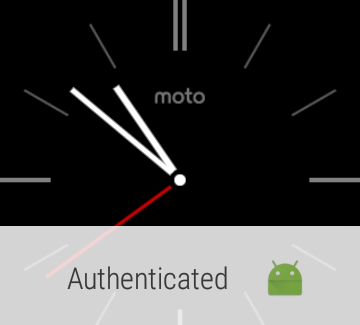
\includegraphics[width=.45\linewidth]{gfx/notification_auth_bar}} \quad
        \subfloat[When selected]
        {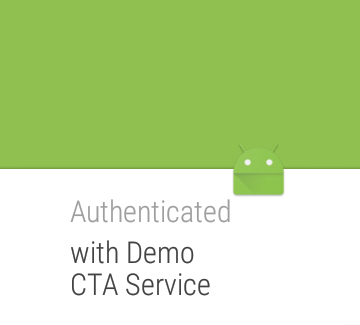
\includegraphics[width=.45\linewidth]{gfx/notification_auth}} 
        \caption{Example of notifications on the watch}
        \label{fig:watch}
\end{figure}

\begin{figure}[bth]
        \myfloatalign
        \subfloat[Registration notification]
        {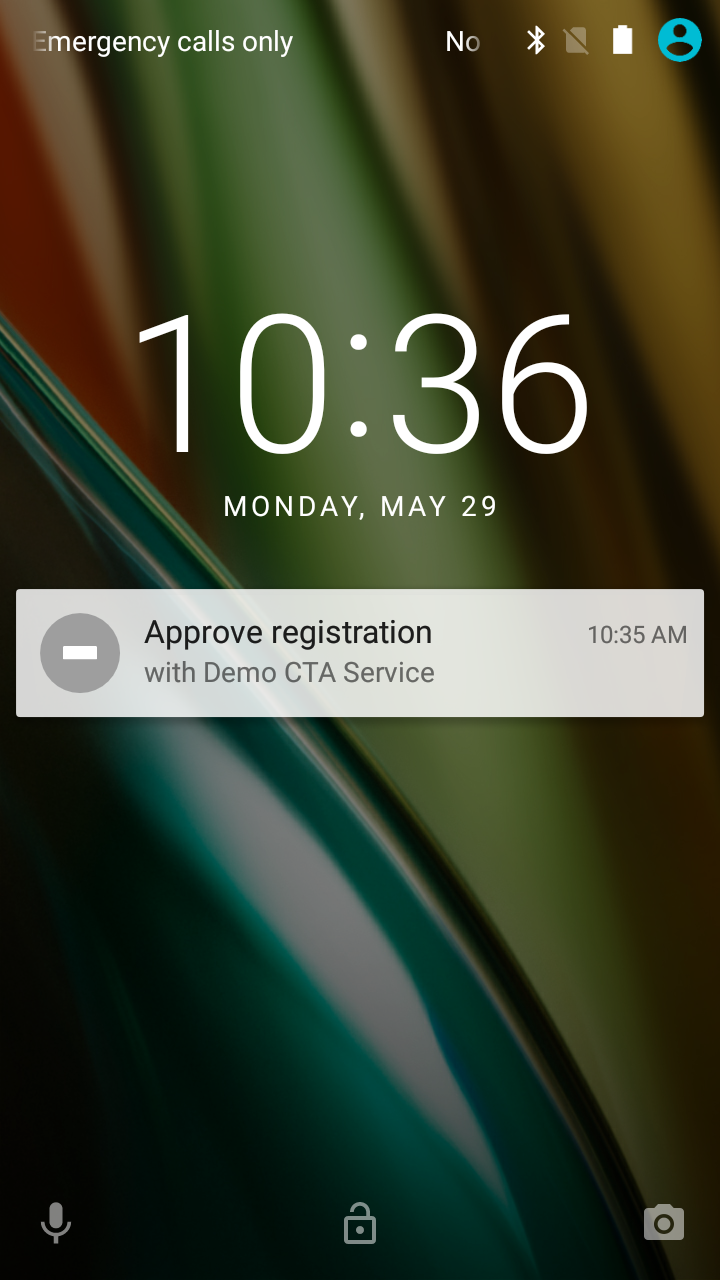
\includegraphics[width=.45\linewidth]{gfx/notification_register_phone}} \quad
        \subfloat[When selected]
        {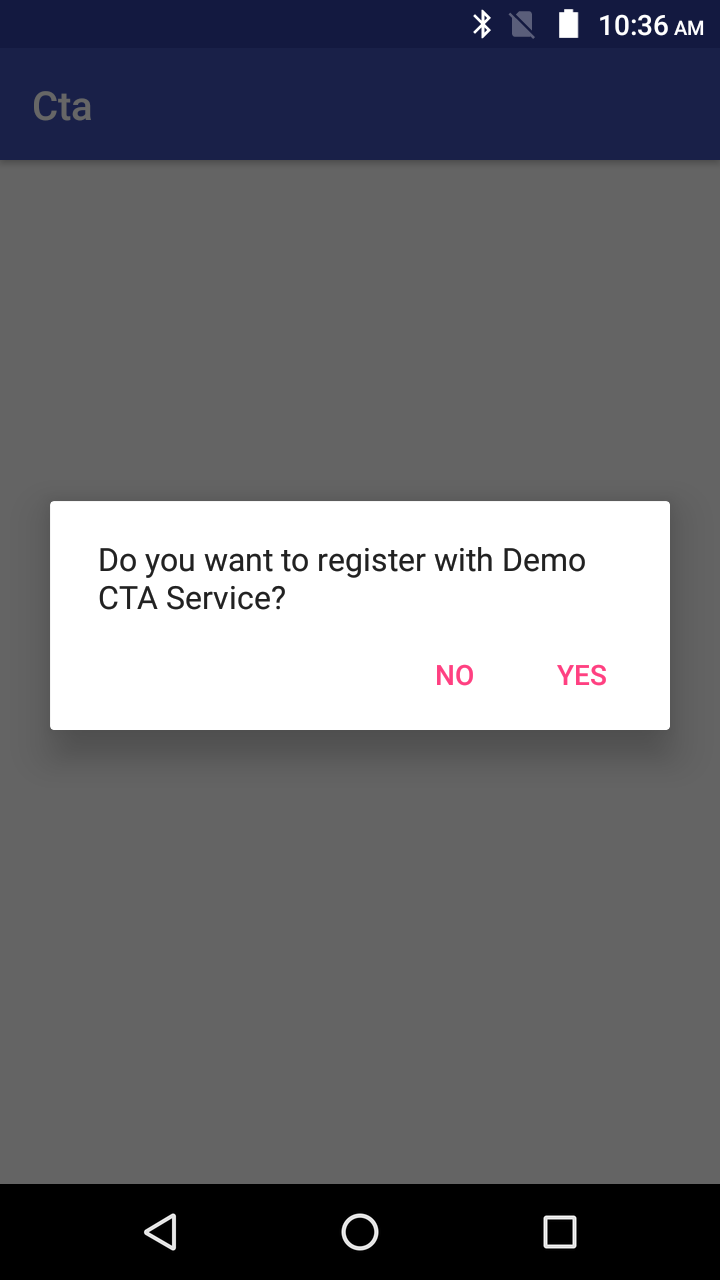
\includegraphics[width=.45\linewidth]{gfx/notification_register_approve}} 
        \caption{Example of explicit consent on the phone}
        \label{fig:phone}
\end{figure}

The \gls{server} is implemented as a server application that receives requests from the \gls{client}. Upon registration requests from the \gls{client}, the server is responsible for checking that the supplied username is available, and not already in use. If available it will respond to the \gls{client}, which will then initiate the registration process as specified in the protocol. Upon authentication requests from the \gls{client}, the server is responsible for encrypting new challenge ciphers and waiting for the \gls{client} to respond back with the correct cleartext message. Upon successful authentication the server generates a new token with a set expiration time, that is returned to the \gls{client}. This token allows the \gls{client} to authenticate with the \gls{server} as long as it is valid.

The \gls{client} is implemented as a small web application that runs in a browser. The \gls{client} is responsible for receiving input from the user, in the form of instructions of when to authenticate and register the user. Before either authentication or registration can be started from the \gls{client}, it must establish a connection with an \gls{authenticator} and a \gls{server} so that it can exchange protocol messages between the two parties. The client provides a simple user interface with a `pair' button used to select the correct \gls{authenticator} from a list of nearby Bluetooth devices. It has a field for typing a username, a button to perform registration and one to perform authentication. It also shows a log for displaying output from the client itself and response messages from its communicating parties. Lastly, it has a button used to interrupt the continuous authentication cycle with the \gls{server}, available whenever the client is authenticated.

\begin{figure}
       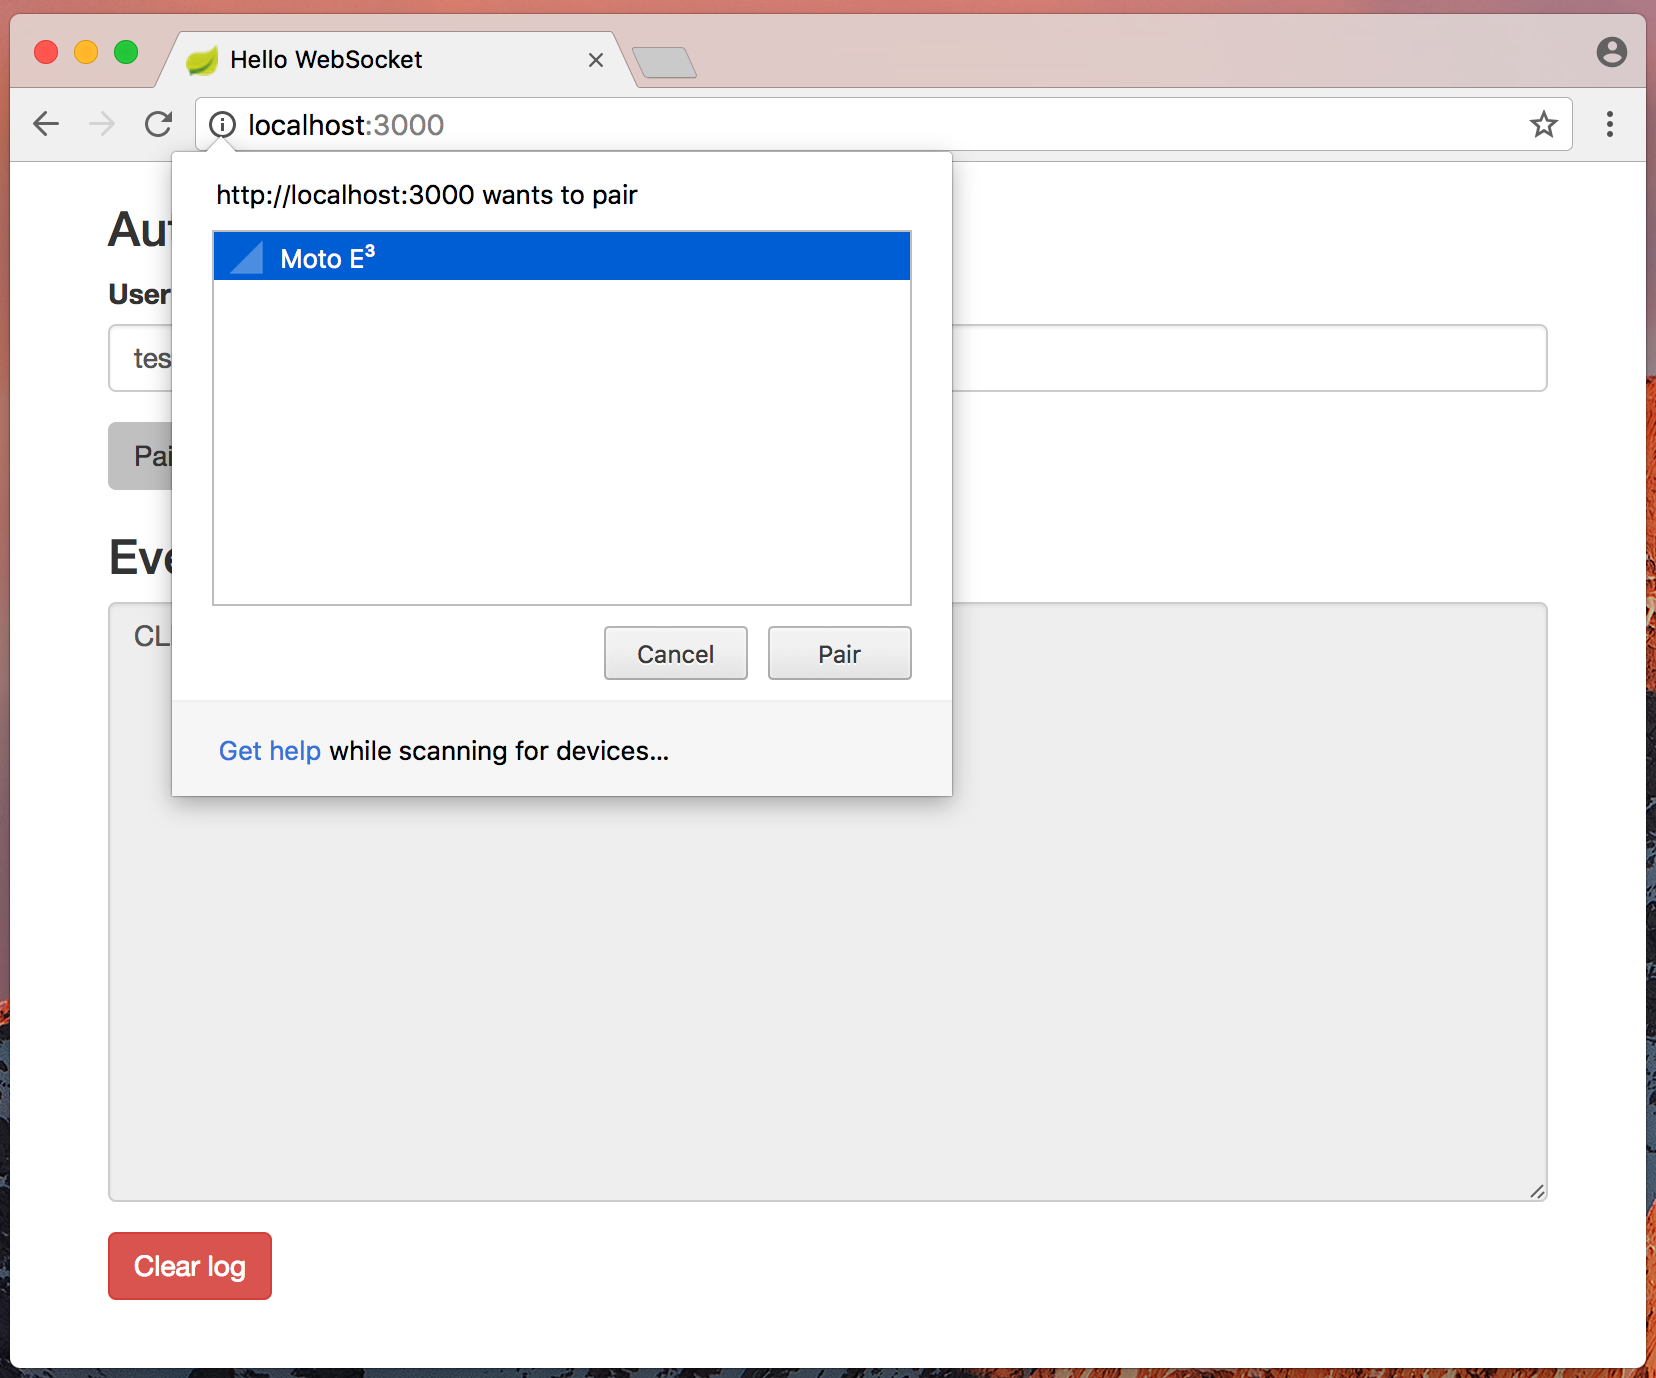
\includegraphics[width=\linewidth]{gfx/paring2} 
       \label{fig:paring}
       \caption{The pairing menu in Chrome}
\end{figure}

\begin{figure}
       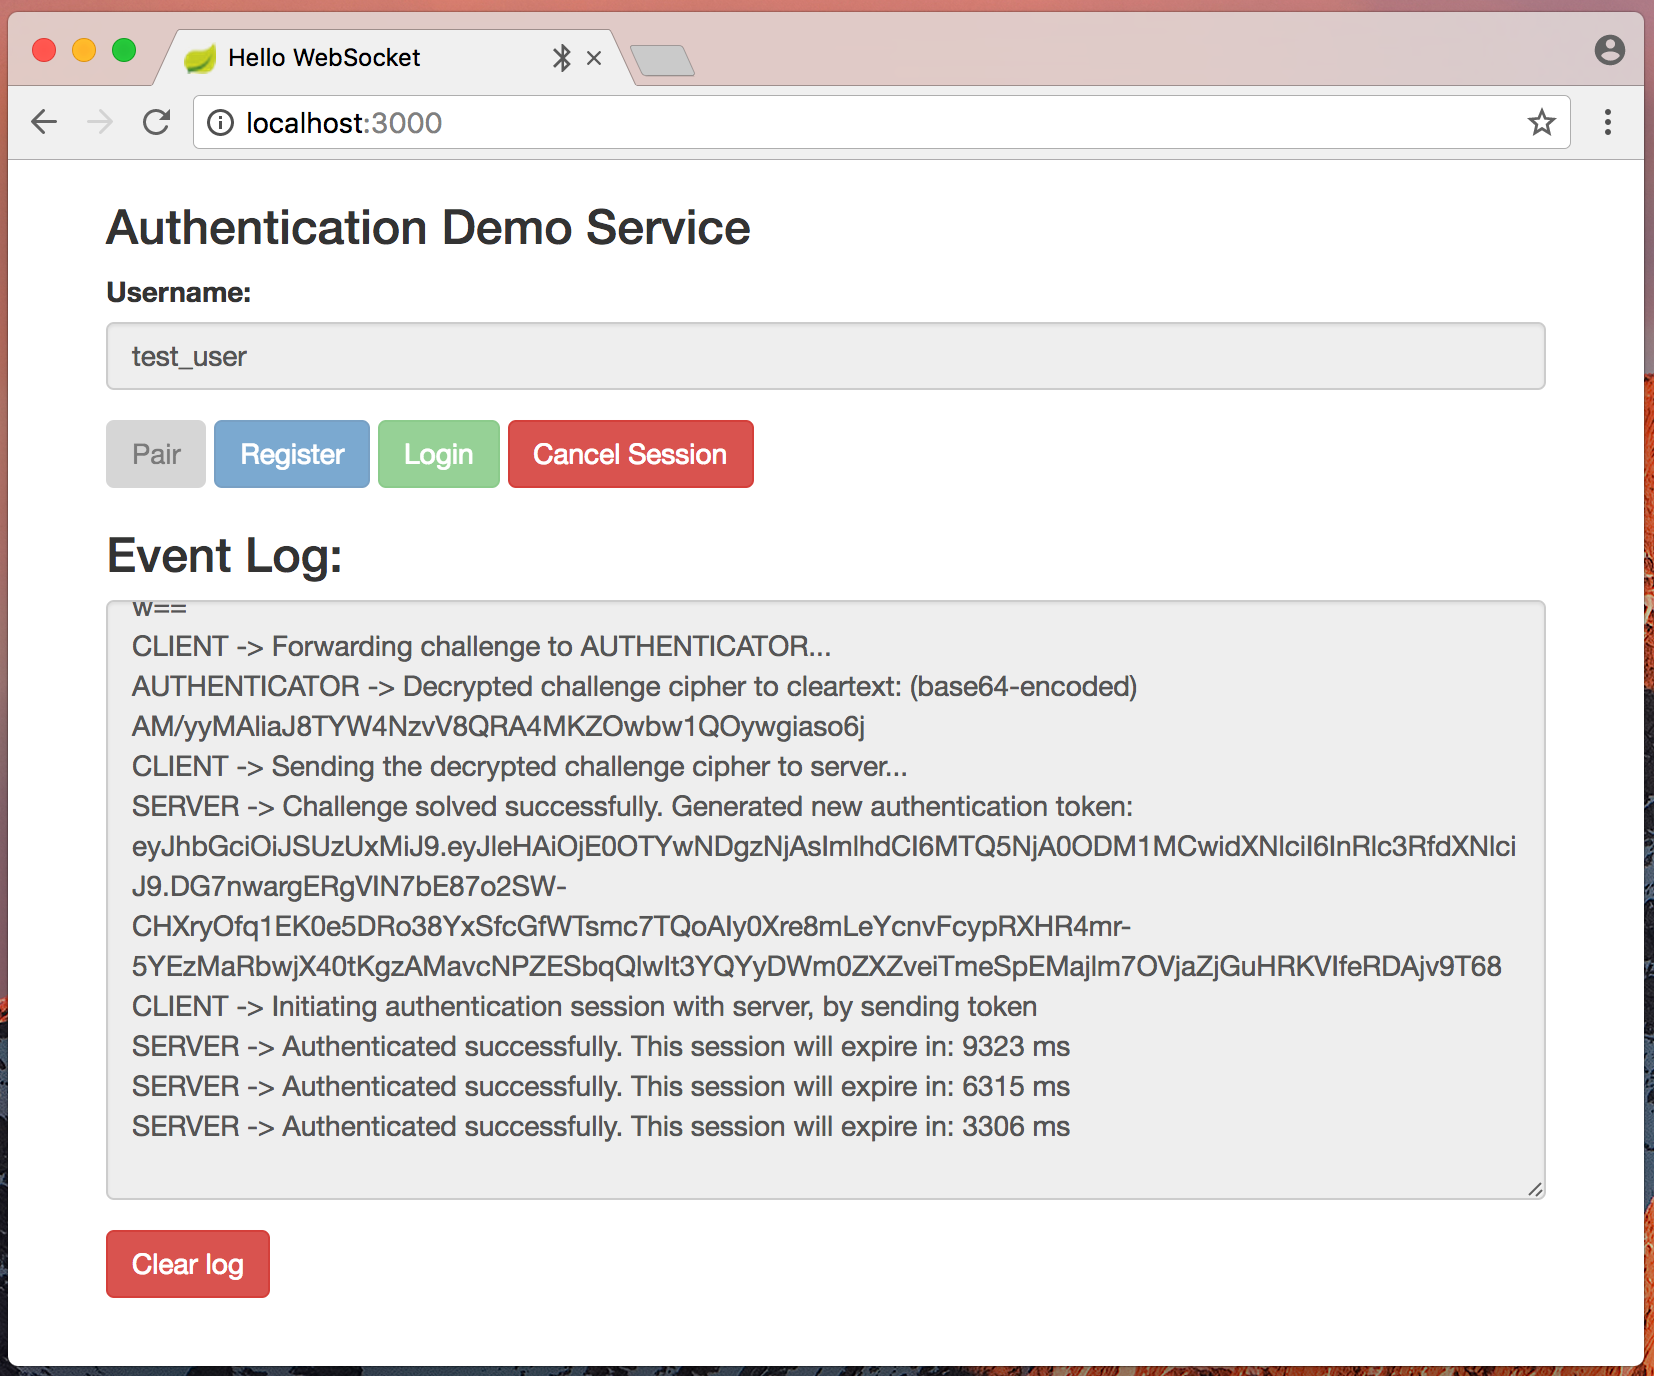
\includegraphics[width=\linewidth]{gfx/login} 
       \label{fig:client}
       \caption{Authenticating with a service in Chrome} 
\end{figure}


\section{Technical Description}
\subsection{Technologies Used}
One clear and important design goal, is to base the prototype implementation of our authentication scheme on commodity hardware and recognized technologies, and as such, this should be clearly reflected in our choice of technologies used. 

The prototype is using the Android platform for the \gls{authenticator} and \gls{sibling}, and developed using Java. All message exchanges between the two devices are handled using the Bluetooth communication protocol. For developing and testing we used Motorolas Moto 360 smartwatch and their $\text{Moto E}^3$ smartphone, although the hardware can be substituted with any two Bluetooth 4.0 LE supported devices that run Android OS and Android Wear OS respectively, with API level 21 or higher. 

The \gls{client} is running a browser application that is served statically as Javascript and HTML files.

We use Bluetooth GATT services to establish a link between \gls{client} and \gls{authenticator}

Generic Attributes (GATT) profile is a feature in Bluetooth LE that allows device discovery based on services without device pairing. A common use of GATT is with sensors, such as heart-rate monitors, that can easily be discovered as used ad-hoc.

We use GATT to expose an authentication service from the \gls{authenticator} that be easily discovered, and can be used without regular device pairing.

Because native GATT service compatibility in the browser is still under active development, the \gls{client} application is only functioning properly in Google Chrome Version 59 or later, which at the time of writing is still in beta release state. When selecting a new unknown device in Chrome for the first time, Chrome as a security requires that the end-user selects the device from a pairing drop-down menu. This is shown in figure~\ref{fig:pairing}. The implementation will, but does not yet support automatically establishing connections to known devices when they come in range.

The \gls{server} is implemented as a server application using Java and the Spring Boot framework. Communication between \gls{client} and server is handled through the WebSocket communication protocol. Public keys user information and generated challenges, are persisted on the server using a MySQL relational database. The server uses the open standard (RFC 7519) JSON Web Tokens (JWT), to issue and verify authentication tokens. The details of token generation and verification are explained in section \ref{sec:tokens} below. 

All cryptographic computations are carried out using the BouncyCastle cryptography Java API. However as the Android platform ships with a limited version of BouncyCastle, and can not be updated to the latest version due to classloader conflicts, we use SpongyCastle to perform cryptographic operations on the \gls{authenticator} and \gls{sibling}. SpongyCastle is essentially the exact same API as BouncyCastle only with a different name, created only with the purpose of enabling the full and updated API of BouncyCastle on the Android platform. The details of our cryptography implementation is explained in section \ref{crypto_impl} below.


\subsection{Algorithms} \label{sec:algorithms}
The implementation of the protocol on the \gls{server}, \gls{authenticator} and \gls{sibling} is based on the algorithms defined below.

\begin{algorithm}
    \BlankLine
    \KwData{Set of public-keys $\{pk_1, pk_2, ..., pk_n \}$}
    \BlankLine
 
    $i \leftarrow recv(C)$
    \tcc*{request from user with id i}
    
    $c = Enc(n,pk_i)$
    \tcc*{generates a random challenge}
    \BlankLine
 
    $send(C,\langle c, i \rangle)$
    \tcc*{sends a challenge to C}
    
    $n' \leftarrow recv(C)$
    \tcc*{receives a response}
    \BlankLine
    
    \If(\tcc*[f]{if the response is valid}){$n = n'$}{
        $send(C, token)$
        \tcc*{then issue a token to C} 
    }
    \BlankLine

 \caption{Service Provider behaviour during authentication}
 \label{alg:servAuth}
\end{algorithm}

\begin{algorithm}
    \BlankLine
    \KwData{Set of key-pairs $\{sk_1, sk_2, ..., sk_n \}$}
    \BlankLine
 
    $\langle c,i \rangle \leftarrow recv(C)$
    \tcc*{receives challenge from C}
    
    $send(As, \langle c, i \rangle)$
    \tcc*{sends challenge to As}
    \BlankLine
    
    $c'_{A} = Dec'(c,sk_{i})$
    \tcc*{partly decrypts}
    
    $c'_{As} \leftarrow recv(As)$
    \tcc*{receives other half from As}
    \BlankLine
    
    $n' = c'_{A} \times c'_{As}$
    \tcc*{combines the parts}
    
    $send(C, n')$ \tcc*{send the token to C}
    \BlankLine
    
 \caption{Authenticator behaviour during authentication}
 \label{alg:authAuth}
\end{algorithm}

\begin{algorithm}
    \BlankLine
    \KwData{Set of private-keys $\{sk_{1}, sk_{2}, ..., sk_{n} \}$}
    \BlankLine
 
    $\langle c,i \rangle \leftarrow recv(A)$
    \tcc*{receives challenge from A}
    
    $c'_{As} = Dec'(c,sk_{i})$
    \tcc*{partly decrypts}
    
    $send(A, c'_{As})$
    \tcc*{sends it to A}
    \BlankLine
    
 \caption{Sibling behaviour during authentication}
 \label{alg:sibAuth}
\end{algorithm}

\clearpage

\subsection{Cryptography Implementation} \label{crypto_impl}
As earlier mentioned, BouncyCastle cryptography API (SpongyCastle on Android) is used, to implement the protocol in practice. 
The different cryptographic operations needed for the \gls{authenticator} and \gls{sibling} are exposed in a shared class which they both use. 
Initially the encryption/decryption scheme to be used, is set to El Gamal without padding, and the bit length is set to 256 for all generated keys (lst. \ref{lst:distEl}, line 47-66). 
 
When a user registers with a new \gls{server}, the \gls{sibling} and the \gls{authenticator} creates an El Gamal key pair each. Key generation is trivial to implement and is handled trough the BouncyCastle API (lst. \ref{lst:distEl}, line 133-152).
To reduce key generation time significantly we avoid generating new large prime numbers required for the El Gamal key parameters $p$ and $g$ each time, but instead uses fixed values for both, that we know are applicable for secure key generation (lst. \ref{lst:distEl}, line 36-37).
When the key pairs are successfully created on each device, the \gls{sibling} sends its public key $y_{as}$ to the \gls{authenticator}, which then adds the \gls{sibling}s public key $y_{as}$ to its own public key $y_a$, resulting in a combined public key $y$ (lst. \ref{lst:distEl}, line 69-85). The \gls{authenticator} now sends its public key $pk$ ($y$ along with parameters $p$ and $g$) to the \gls{server}, where it is stored and associated with the registering user. 

When an authentication request is initiated by the user, the server application encrypts a new challenge cipher, based on the public key it received upon registration. 
The challenge is generated using the formula $(h^2 ~\mathrm{mod}~p)$ where $h$ is an arbitrary integer of $\mathbb{Z}^*_p$ in the range $\big\{ 2, ..., p-2 \big\}$. Naturally, the server also uses the El Gamal No Padding cipher to perform encryption. The server stores the challenge in the database in both cleartext and ciphertext along with an expiration timestamp indicating how long the \gls{server} accepts responses for the generated challenge (lst. \ref{lst:chalService}, line 46-81). 

The challenge is sent to the \gls{authenticator}, which will now decrypt the cipher in cooperation with its \gls{sibling}. As shown in algorithm: \ref{alg:authAuth}, the \gls{authenticator} sends a copy of the challenge to the \gls{sibling} immediately upon receiving it from the server. Hereafter both devices will perform a partial decryption of the cipher, using their individual private key. This is done by first splitting the challenge cipher into two parts: $\alpha$ and $\beta$ (lst. \ref{lst:chalService}, line 168-181). Partial decryption is then done by: $\left[\beta^{(p-1-x)} ~\mathrm{mod}~p\right]$, where $x$ is the private key, and $p$ is the common security parameter of the public key (lst. \ref{lst:chalService}, line 98-109). Note that, as $p-1$ is the order of the group used, then $h^{(p-1)} = 1$ with $h \in \mathbb{G}$.
\begin{align*}
    && c'_i = \beta^{(p-1-x_i)} = \frac{\beta^{(p-1)}}{\beta^{x_i}} = \beta^{-x_i}
\end{align*}

Note that this is different from the partial decryption as defined in the protocol section. This is due to the fact that division in groups in Bouncy Castle is defined as $a / b \stackrel{def}{=} \left[ ab^{-1}~\mathrm{mod}~p \right]$.

The main difference between the algorithm  executed by the \gls{authenticator} (algorithm~\ref{alg:authAuth}) and the one (algorithm~\ref{alg:sibAuth}) executed by the \gls{sibling}, is that the \gls{sibling} sends the result of its decryption directly to the \gls{authenticator}, which combines the two partial ciphers into the correct cleartext solution of the challenge. The \gls{authenticator} does so by computing $\left[\alpha \cdot c'_1 \cdot c'_2 ~\mathrm{mod}~p\right]$ where $c'_1$ and $c'_2$ are the partial ciphers from the \gls{authenticator} and \gls{sibling} (lst. \ref{lst:chalService}, line 87-96). This formula computes the solution to the challenge, which is then sent back to the server, so it can complete the last step of its algorithm (algorithm~\ref{alg:servAuth}), which is to authenticate the \gls{client}.


\subsection{Token Issuing and Verification} \label{sec:tokens}
The prototype is using JSON Web Tokens (jwt.io), to issue new authentication tokens on the server, upon receiving a correct solution to a challenge. The tokens are signed digitally with a public/private key pair using RSA. JWT tokens can carry different kinds of information with them, such as a timestamp to indicate an expiration time for the token. 
Our implementation uses the JWT Java API provided by Auth$0$(\href{https://github.com/auth0/java-jwt}{GitHub page}). The server generates a new RSA key pair upon server start (lst. \ref{lst:tokenService}, line 37-52). When a new token has to be issued for a given user, the following information is stored in the token: a timestamp for when the token was issued, a timestamp for when the token is set to expire, the username of the authenticated user. The token is then signed with RSA512 using the private key that was generated on server start (lst. \ref{lst:tokenService}, line 54-73). Verification is done using the RSA public key. The verification function of the API takes an RSA public key as input, and checks and that the token is signed by the corresponding private key and not expired yet (lst. \ref{lst:tokenService}, line 75-93). 


\section{Prototype Evaluation}\label{sec:prot_eval}
We evaluate our implementation based on the framework proposed by \citet{bonneau2012quest}, in a similar manner to how we evaluated the design of our scheme in section \ref{sec:rating_process}, and other schemes in chapter \ref{ch:review}. 

\begin{table}[bth]
\centering
\begin{wide}
\resizebox{\linewidth}{!}{
%\rotatebox{270}{
\setlength\tabcolsep{1.8pt}
\begin{tabular}{r|c|cccccccccc|cccccc|ccccccccccccc}

\multicolumn{2}{c}{} &
\multicolumn{10}{c}{\textbf{Usability}} &
\multicolumn{6}{c}{\textbf{Deployability}} &
\multicolumn{13}{c}{\textbf{Security}}\\
\multicolumn{31}{c}{}
\\

& \rot{\textit{Reference}} &
\rot{\textit{Memorywise-Effortless}} &
\rot{\textit{Scalable-for-Users}} &
\rot{\textit{Nothing-to-Carry}} &
\rot{\textit{Physically-Effortless}} &
\rot{\textit{Easy-to-Learn}} &
\rot{\textit{Efficient-to-Use}} &
\rot{\textit{Infrequent-Errors}} &
\rot{\textit{Easy-Recovery-from-Loss}} &
\rot{\textit{Awareness}} &
% \rot{\textit{Multi-User-Support}} &
\rot{\textit{No-Config}} &
\rot{\textit{Accessible}} &
\rot{\textit{Negligible-Cost-per-User}} &
\rot{\textit{Server-Compatible}} &
\rot{\textit{Browser-Compatible}} &
\rot{\textit{Mature}} &
\rot{\textit{Non-Proprietary}} &
\rot{\textit{Resilient-to-Physical-Observation}} &
\rot{\textit{Resilient-to-Targeted-Impersonation}} &
\rot{\textit{Resilient-to-Throttled-Guessing}} &
\rot{\textit{Resilient-to-Unthrottled-Guessing}} &
\rot{\textit{Resilient-to-Internal-Observation}} &
\rot{\textit{Resilient-to-Leaks-from-Other-Verifiers}} &
\rot{\textit{Resilient-to-Phishing}} &
\rot{\textit{Resilient-to-Theft}} &
\rot{\textit{No-Trusted-Third-Party}} &
\rot{\textit{Requiring-Explicit-Consent}} &
\rot{\textit{Unlinkable}} &
\rot{\textit{No-Intermediary-Knowledge}} &
\rot{\textit{Continuous}} \\ \hline

Scheme design & &
\CIRCLE     & %Memorywise-Effortless
\CIRCLE     & %Scalable-for-Users
\Circle     & %Nothing-to-Carry
\CIRCLE     & %Physically-Effortless
\CIRCLE     & %Easy-to-Learn
\CIRCLE     & %Efficient-to-Use
\CIRCLE     & %Infrequent-Errors
            & %Easy-Recovery-from-Loss
\CIRCLE     & %Awareness
%           & %Multi-User-Support
            & %No-Pairing
\CIRCLE     & %Accessible
\Circle     & %Neglible-Cost-per-User
            & %Server-Compatible
            & %Browser-Compatible
            & %Mature
\CIRCLE     & %Non-Proprietary
\CIRCLE     & %Resilient-to-Physical-Observation
\CIRCLE     & %Resilient-to-Targeted-Impersonation
\CIRCLE     & %Resilient-to-Throttled-Guessing
\CIRCLE     & %Resilient-to-Unthrottled-Guessing
\Circle     & %Resilient-to-Internal-Observation
\CIRCLE     & %Resilient-to-Leaks-from-Other-Verifiers
\CIRCLE     & %Resilient-to-Phishing
\Circle     & %Resilient-to-Theft
\CIRCLE     & %No-Trusted-Third-Party
\Circle     & %Requiring-Explicit-Consent
\CIRCLE     & %Unlinkable
\CIRCLE     & %No-Intermediary-Knowledge
\CIRCLE       %Continuous
\\ \hline

Prototype Implementation & \cite{stajano2011pico} &
\CIRCLE     & %Memorywise-Effortless
\CIRCLE     & %Scalable-for-Users
\Circle     & %Nothing-to-Carry
\CIRCLE     & %Physically-Effortless
\CIRCLE     & %Easy-to-Learn
\Circle     & %Efficient-to-Use
\CIRCLE     & %Infrequent-Errors
            & %Easy-Recovery-from-Loss
\CIRCLE     & %Awareness
%           & %Multi-User-Support
\CIRCLE     & %No-Pairing
\CIRCLE     & %Accessible
\Circle     & %Neglible-Cost-per-User
\Circle     & %Server-Compatible
\Circle     & %Browser-Compatible
            & %Mature
\CIRCLE     & %Non-Proprietary
\CIRCLE     & %Resilient-to-Physical-Observation
\CIRCLE     & %Resilient-to-Targeted-Impersonation
\CIRCLE     & %Resilient-to-Throttled-Guessing
\CIRCLE     & %Resilient-to-Unthrottled-Guessing
\Circle     & %Resilient-to-Internal-Observation
\CIRCLE     & %Resilient-to-Leaks-from-Other-Verifiers
\CIRCLE     & %Resilient-to-Phishing
\Circle     & %Resilient-to-Theft
\CIRCLE     & %No-Trusted-Third-Party
\Circle     & %Requiring-Explicit-Consent
\CIRCLE     & %Unlinkable
\CIRCLE     & %No-Intermediary-Knowledge
\CIRCLE       %Continuous
\\ \hline
\multicolumn{31}{r}{

\CIRCLE~=~offers the benefit 
\quad \Circle~=~almost offers the benefit
%\quad \textit{no circle}~=~does not offer the benefit 
\quad ?~=~not known}
\quad \\

\end{tabular}}
\end{wide}

\caption[Overview of benefits of our prototype]{Comparing the (envisioned) benefits of our design with the actual benefits of our implementation.}
\label{table:property_table2}
\end{table}

\subsection{Rating process}
To avoid repeating ourselves, we only describe the rating rationale behind the specific benefits of the prototype implementation that differ from the scheme design. 
We grant the prototype \textit{No-Config} as it actually offers this benefit according to our definition, since there is no difference between the required effort from the user, the first time or sub sequential times it is used on any client. This may appear more beneficial than it actually is. In reality, a pairing step between \gls{authenticator} and \gls{client}, becomes something the user has to do every single time he starts a new authentication or registration request, instead of something that should only be done once on each \gls{client}, which obviously is less desirable. This is also the reason why we only grant the prototype \textit{Quasi-Efficient-to-Use} as the user is required to select the correct \gls{authenticator} from a list of devices, on the \gls{client}, every time the browser reloads the page. 
While deployability benefits are not prioritized in the scheme design, it was discovered during implementation that it was actually possible to achieve both \textit{Browser-} and \textit{Server-Compatibility} to some extent. We award the prototype \textit{Quasi-Browser-Compatibility} as no browser plugins or additional software is required to run on the \gls{client} machine, in order to use the prototype. However the browser support for Bluetooth GATT services is used in the implementation, is still in a beta state, and currently only works in a limited amount of browsers. Assuming that Bluetooth communication directly through the browser, becomes more common and widely supported in the future, we award \textit{Quasi-Browser-Compatibility}.
We award \textit{Quasi-Server-Compatibility}, since servers that already use JWT tokens for authentication, can become compatible with the scheme, without a complete re-implementation of its authentication infrastructure . 
Essentially such servers do not require changes, in terms of how it is determined whether a user is authorized to access a requested resource or not. Instead, a change is needed, in the way it is determined whether a user is entitled to receive an authentication token or not, which today is typically done by verifying a user's username/password credentials. 

\cleardoublepage
\part{Discussion \& Conclusion}
%************************************************
\chapter{Discussion}\label{ch:discussion}
%************************************************

\section{Security Assumptions and Attacks} \label{sec:attacks}

In the security analysis, we analyzed the proposed protocol and showed that the protocol has an injective agreement in the presence of adversaries capable of \textit{Internal Observation}. However, we also showed that if an adversary is capable of \textit{Strong Internal Observation}, then he can mount an attack as shown in figure~\ref{fig:attacks}.

So far we have not discussed the implications of this attack. Most realistically this attack can be mounted by compromising the \gls{authenticator}, as this will give the adversary access to both the key, and the communication to the \gls{sibling}. With control of the network, the adversary can send packages to the \gls{sibling} and make it partially decrypt selected ciphers.

\begin{figure}[bth]
    \centering

    %\begin{wide}
    \begin{minipage}[c]{0.49\linewidth}
    \resizebox{\linewidth}{!}{
    \begin{msc}{Authenticator compromised}
    
    \setlength{\instdist}{1.7cm}
    \setlength{\envinstdist}{1.7cm}
    \setlength{\actionwidth}{3cm}
    
    \declinst{as}{$\left\{sk_{As}\right\}$}{$As$} 
    \declinst{a}{}{$\mathcal{A}$} 
    
    \nextlevel
    
    \mess*{$\left\{c\right\}$}{envright}{a}
    \nextlevel
    
    \action{$sk_A = LtkReveal(A)$}{a}
    \nextlevel[4]
    
    \mess{$\left\{c\right\}$}{a}{as}
    \nextlevel
    \action{$c'_{As} = Dec'(c,sk_{As})$}{as}
    \action{$c'_{A} = Dec'(c,sk_{A})$}{a}
    \nextlevel[5]
    \mess{$\left\{c'_{As}\right\}$}{as}{a}
    \nextlevel
    \action{$n' = c'_A \times c'_{As}$}{a}
    \nextlevel[3]
    \mess*{$\left\{n'\right\}$}{a}{envright}
    \end{msc}}
    \end{minipage}
    %
    \begin{minipage}[c]{0.49\linewidth}
    \resizebox{\linewidth}{!}{
    \begin{msc}{Sibling compromised}
    
    
    \setlength{\instdist}{1.7cm}
    \setlength{\envinstdist}{1.7cm}
    \setlength{\actionwidth}{3cm}
    
    \declinst{as}{}{$\mathcal{A}$} 
    \declinst{a}{$\left\{sk_{A}\right\}$}{$A$} 
    \nextlevel
    
    \mess*{$\left\{c\right\}$}{envright}{a}
    \nextlevel
    
    \mess{$\left\{c\right\}$}{a}{as}
    \nextlevel
    
    \action{$sk_{As} = LtkReveal(As)$}{as}
    \nextlevel[4]
    
    \action{$c'_{As} = Dec'(c,sk_{As})$}{as}
    \action{$c'_{A} = Dec'(c,sk_{A})$}{a}
    \nextlevel[5]
    
    \mess{$\left\{c'_{As}\right\}$}{as}{a}
    \nextlevel
    
    \action{$n' = c'_A \times c'_{As}$}{a}
    \nextlevel[3]
    
    \mess*{$\left\{n'\right\}$}{a}{envright}
    \end{msc}}
    \end{minipage}
    %\end{wide}
    \caption[Sequence diagrams of known attacks]{The known attacks by adversaries capable of Strong Internal Observation}
    \label{fig:attacks}
\end{figure}

So what does the adversary gain from this attack? The response to a challenge could be obtained much easier by eavesdropping the plain-text nonce when it is sent from \gls{authenticator} to the \gls{client} and then to the \gls{server}. Furthermore, the user is still able to stop further authentications by removing the \gls{sibling} from the \glspl{authenticator} proximity, or simply turning it off.

This is proven as: For all successful rounds of authentications, if an adversary is limited to a proper subset of keys, then either the \gls{authenticator} or \gls{sibling} was involved in the authentication run (as defined in section~\ref{sec:involvement}).

This is an important property as, even if some subset of devices are compromised, then the user retains the ability to stop all current and future authentications by turning off the device, or putting the device on lockdown. Recall that this was one of the scenarios presented in the design (see table~\ref{sc:theft}).

However, a more severe consequence of the attack; In the protocol design session we stated that hijacking a session should not give an adversary unauthorized access for longer than the session is actively kept alive by the \gls{authenticator} and \gls{server}. The attack would violate this goal as it allows the adversary to omit the \glspl{authenticator} logic and keep a session alive even after the \gls{authenticator} is locked (e.g. if it is not worn). Furthermore, if the adversary can compute the response to a challenge, and thus omit user-awareness, explicit consent and other checks and bounds implemented on the authentication, then it undermines many of the user-oriented security features that our design presents.

In the current version of the protocol, no messages sent are authentic. As we have shown that the known attacks can be mitigated by having authentic communication, future work should include to further analyze and extend the protocol to have message authenticity.\\

In the security analysis, registration is assumed to be an atomic operation. This is, of course, not the case in practice. The registration is, as most key-exchanges are, vulnerable to man-in-the-middle attacks. Password-based authentication also suffers from this problem, and a common fix is to use secure channels such as HTTPS.
However, for our protocol, securing the communication between \gls{client} and \gls{server} with HTTPS, only partly mitigates the attack surface. It is left for future work to analyze and prevent man-in-the-middle attacks between \gls{client}, \gls{authenticator} and \gls{sibling} during registration.

% An implication of this definition is that a device is either acting or not acting in a run of the protocol. In practise, an adversary could also compromise the device, and not be able to obtain the key, but instead e.g. always accept explicit consent request without any user interaction. This could lead to attacks, but is not entailed by the model. This will be revisited in the discussion.

\section{Confidence in Tamarin}

As we pointed out both in this chapter and in the security analysis, two strategies for compromising the protocol are known. Both attacks assume that an adversary is capable of \textit{Strong Internal Observation}, and is thus able to compromise the keys of one actor, and to break message authenticity and secrecy. The two attacks are shown in figure~\ref{fig:attacks}. 

While both attacks can be mounted by adversaries capable of \textit{Strong Internal Observation}, and thus disprove proposition~\ref{proposition:forge-rev-in} in our computational model, we have discovered that Tamarin does not find the second attack where the attack is mounted by compromising the key of the \gls{sibling}. 

Although the adversary has all the knowledge and rules available to mount the attack; it does not discover the attack unless a rule explicitly stating the strategy is given in the model
\begin{align*} 
&& In(c),~In(x),~In(p) \ifarrow Out(comb(pdec(c,x), p)) 
\end{align*}

It should be clear from the rule that an adversary with the information necessary to invoke the rule,
\begin{align*}
    %pk &= comb(pk(x), pk(y)) && (\text{from register}) \\
    c &= enc(n, pk) && (\text{from  server-init}) \\
    p &= pdec(c,y) && (\text{from sibling})\\
    x & && (\text{from reveal})
\end{align*}
with $pk = pk(plus(x,y))$, should already be to able obtain $n$ given our equational theory.
\begin{align*}
&    dec(enc(m,pk(sk)), sk) \simeq m\\
&    comb(pdec(c,x), pdec(c,y)) \simeq dec(c,pk(plus(x,y)))
\end{align*}

However, the attack is only found if the rule is explicitly present in the model. We have been in contact with the developer of Tamarin who confirms that it seems to be a bug in the tool\footnote{\url{https://github.com/tamarin-prover/tamarin-prover/issues/216}}. 

This naturally lead us to question the validity of the proofs given in section~\ref{sec:tamarin}. We are, even considering the bug, confident that the given theorems of unforgeability and injective agreement holds. However, we suggest for future work to prove the theorems with a different tool or model to obtain certainty hereof.



\section{Trusted Input, Output and Computations}

In the security analysis we proved that the protocol achieves unforgeability in the presence of \textit{Strong External Observation}, and as such, if an adversary can not obtain any of the secret keys, then unforgeability is proven. So can we make an implementation where we can reasonably assume that adversaries are only capable of \textit{Strong External Observation}?

A way to ensure the secrecy of the keys is to use TPM. In his thesis \citet{bentzon2013security} showcases an implementation of Pico that mitigates the risk of the Pico being compromised in an unlocked state by using a Trusted Platform Module (TPM), which are small special purpose hardware chips that allow for compartmentalization, as both keys and cryptographic calculations can be carried out in separation from the operating system.

TPM modules are standard in most commodity devices such as laptops and phones, and using a TPM for storing the keys and performing the cryptographic calculations is an effective means of mitigating the risk of compromised devices.

However, as hinted previously, a flaw in the way we modeled and proved our protocol is that the definition of an actors involvement is too binary. In practice, we have so far been assuming trusted input and output. This means we assume that if the authenticator acted, then user-awareness, explicit-consent and other checks and bounds was actually performed. However, even if an adversary is not able to compromise the secrets of the system, he might be able to compromise the user in- and output. As we have already explained above, this can have serious ramifications for the user-oriented security features of our scheme. 

We therefore suggest for future work to include exploring how trusted input, -output and -computations can be used to mitigate the risk of attacks.

\section{Number of Siblings}

The concept of siblings is crucial to our design as it mitigates the risk of both theft and compromised devices. By splitting the secrets onto multiple devices, we make it more difficult for an adversary to mount an attack. 

The concept originates from the Pico~\cite{stajano2011pico, stannard2012good}. However, in contrast to our design, multiple siblings are suggested. This lead us to an interesting discussion point: How many devices should the user be obligated to have in his vicinity?

\citet{stajano2011pico} suggests that siblings could be items such as glasses, belts, wallets, jewelry and possible implants. Our design choice of using only one sibling stems from a practical consideration. Forcing the user to always have both watch and smartphone present when authenticating is already a significant trade-off.

However, we do see the potential in having the number of siblings as a variable parameter of security. In fact, our protocol naturally supports having more than one sibling as Distributed ElGamal works for any number of participant, and the scheme could easily be extended to allow more siblings.\\

Pico uses a $k$-out-of-$n$ threshold encryption scheme allowing a user to authenticate even though some siblings are not present. There are multiple interesting aspects to this: there is the natural benefit of allowing the user to forget one of multiple devices, but even more interestingly it could be used as a recovery mechanism where if the user losses e.g. one out of two siblings in a 2-out-of-3 system, then still having the majority of devices could allow the user to replace a lost device.

Our current use of Distributed ElGamal enforces that all devices are bound to participate. However, Distributed ElGamal can quite elegantly be extended to a $k$-out-of-$n$ threshold encryption system by choosing a joint private-key $x$, and then dealing it into several shares $x_1, ..., x_n$ with Shamir's secret sharing scheme~\cite{shamir1979share}. This would allow for computing partial decryptions as we already do, but only needing $k$-out-of-$n$ shares to recover the message~\cite[page 506]{katz2014introduction}.

\section{Recovery Problem}\label{sec:recovery}
The current design of our scheme does not include any proper solution to how a user can recover from a loss of a \gls{sibling} or \gls{authenticator}. As described in the user scenario for theft and loss (\ref{sc:theft}), we envision that a user can initiate a lockdown state, if either of his devices gets stolen or lost. The lockdown state will render both devices useless, until the lockdown state is explicitly canceled by the user, in the event that the lost device resurfaces. However, this idea only considers the case where \textit{one} of the devices is lost, and what happens if the lost device never resurfaces? Surely some recovery mechanism must be put in place that allows replacement of the lost or stolen devices, so that the user can regain control of his web service accounts. The challenge of designing such a mechanism is to make sure that only the legitimate user is allowed to perform recovery. Obviously, it would be catastrophic if an attacker could abuse the recovery process, to gain access and lock out a legitimate user. 

We believe that we have yet to discover the ideal solution for this problem if any such exists. Taking inspiration from Pico's solution to this problem \cite{stajano2011pico}, we have considered the concept of a recovery docking station, that can be placed at the user's home. When the \gls{authenticator} and \gls{sibling} are physically plugged into the dock, all the cryptographic keys contained on the devices are transferred onto the docking station, to be used for recovery later. This way it will be fairly easy, for a user to perform recovery once he is at the recovery station. However, this solution is still problematic in the case where both devices are lost or stolen, since a thief in possession of two stolen devices now has the required equipment to perform authentication. 
One solution to this problem could be to introduce a trusted third party, in the form of a centralized server, that basically acts as a second \gls{sibling}. The \gls{authenticator} would then have to contact the third party and request a partial decryption from it, in order to successfully authenticate with the \gls{server}. The \gls{authenticator} must sign its request, such that the third party can verify that the request is coming from the \gls{authenticator} carried by the legitimate user. Introducing a third party makes it easier to perform lockdown for a user, if both his \gls{authenticator} and \gls{sibling} is lost. If a user performs recovery, the third party can then be instructed to only answer requests from the new \gls{authenticator} used for recovery, instead of the stolen or lost \gls{authenticator}. 

To make sure that it actually is the legitimate user who performs this recovery process, a text- or QR-code could be stored on the recovery station, which must be supplied to the trusted third party, before it can be instructed to answer requests from a new \gls{authenticator}.
In order to view this code or transfer the backup keys onto a new device, the recovery station could, for instance, be protected with a PIN code or a fingerprint scanner. 

At this point, it should be obvious that the problem of recovery is not trivial to solve. While a solution such as the one described above could make recovery viable, it is still far from ideal, as it introduces a new weakest link in the scheme (stealing the recovery station), and furthermore increases the overall cost of deployment, due to the manufacturing cost of the recovery station, and the server maintenance expenses from using a trusted third party.

\section{Reflecting on Evaluation Results}
The evaluation results of the proposed design (figure~\ref{table:property_table}) indicate that the scheme generally performs very well in both security and usability aspects. The main concern in the usability area when compared with related schemes, is that our design does not entail a solution for recovery in case of loss. This problem is discussed above in section~\ref{sec:recovery}. In the area of security, the most significant shortcoming is the lack of full \textit{Resilience-to-Internal-Observation}. This issue is discussed in both chapter~\ref{ch:security} and above in section~\ref{sec:attacks}.
Comparing our proposed authentication scheme with passwords, which is the scheme that is ultimately the target for replacement, we notice the significant lack of provided deployability benefits. As already explained in section~\ref{sec:why} one of the main reasons why passwords have not been replaced on a global scale, is because of its maturity, the fact that it is nearly cost free, and the enormous dependency that exists on passwords in current browser and server infrastructures. In other words it is deployability properties.

With this thesis, we have clearly stated that the proposed scheme is intended as a password replacement. One could therefore rightfully ask why we design the scheme with such small emphasis on deployability, if the lack of deployability is so detrimental to a schemes chance of being widely adopted or contesting passwords in any way. 
The short answer is that full browser and server compatibility is basically only possible to achieve, if the scheme is an abstraction over passwords, such as password managers or a supplement to passwords such as two-factor authentication methods. These solutions have the drawback, that in the end, the weakest link will still be passwords, and such solutions therefore still inherit several of the undesirable security issues that passwords entail. 

We strongly believe that a clean-slate solution is the only way to get completely rid of passwords and achieve optimal security and usability simultaneously. We realize this comes at the significant cost of changes to many browser and server implementations. However, when implementing our prototype, we discovered that it was actually possible to reduce a number of changes needed on both servers and browsers to some extent (see section~\ref{sec:prot_eval}). As many servers are already using a token authentication system, it is possible to only substitute the part of server implementation that issues tokens, and keep the rest of the infrastructure intact. Furthermore, the recent advancements in the compatibility of Bluetooth GATT Service in browsers, enables our scheme to work without implementation changes to browsers. 

While the scheme we propose may require some implementation changes to existing infrastructure, and a more broad adoption of wearable devices, it still provides major improvements in almost all other aspects compared to passwords.



\begin{comment}
\begin{itemize}
    \item Design discussion points:
        \begin{itemize}
            \item Recovery from loss
            \item How good are the properties actually for evaluation? (problems with the framework). 
            \item Comment on evaluation results of design. (lack of deployability benefits)
        \end{itemize}
    \item Prototype discussion points:
        \begin{itemize}
            \item Potential security vulnerabilities
            \item Verify issued tokens on authenticator?
            \item GATT service problems/limitations (mention why we use phone as authenticator)
            \item other technical challenges
            \item comment on evaluation results of prototype (overall satisfaction with prototype)
        \end{itemize}
    \item Protocol:
        \begin{itemize}
            \item TPM's can be used to secure keys
            \item Number of siblings
            \item Partial vs. Threshold encryption
            \item Message integrity
                \begin{itemize}
                    \item An authenticator might be fooled into thinking he is authenticated with a given service. (Also because there is no response from the server)
                    \item Authenticity between sibling and authenticator.
                \end{itemize}
            \item Registration is vulnerable to M-I-M.
        \end{itemize}
\end{itemize}
\end{comment}

% todo
% - 
%************************************************
\chapter{Conclusion}\label{ch:conclusion}
%************************************************

% Motivation and topic
The motivation for this thesis has been to identify or propose a replacement to password-based authentication. Password-based authentication is the most commonly used end-user authentication mechanism, although research concludes it to be insecure and user-unfriendly.
Within the field of pervasive computing, the search for a more user-friendly and unobtrusive authentication method, has long been a topic of research, as the amount of computers a user interacts (and eventually authenticates) with, on a daily basis, is steadily increasing. 

% What we learned from related work
In our work we reviewed and analyzed some existing and relevant pervasive authentication schemes, to gain insights into what works well, and what needs improvement. The solutions we surveyed \cite{stajano2011pico, ojala2008wearable, bardram2003context} are research solutions that are not mature, and all lack a proper implementation. Another observation is that existing solutions tend to rely on dedicated and expensive hardware to facilitate the authentication and furthermore place a primary focus on usability aspects, and prioritize security and cryptographic considerations to a lesser extent. 

% What have we done in this project?
Based on the review, this thesis presents a new password-less authentication scheme, designed to rely on commodity hardware (wearables), and includes and extends upon some of the well working concepts from existing work, such as user awareness, continuous and transparent authentication, in order to achieve a high degree of both usability and security. We describe a well specified and formally verified authentication protocol, that can facilitate the scheme in a secure manner, and provide a thorough documentation of the verification process along with a security analysis of possible vulnerabilities and attacks. 

Based on the design, a working prototype is developed, that serves to demonstrate successful rounds of continuous authentication using our specified protocol. The developed prototype certainly fulfills the goal of avoiding dedicated and special purpose technology as it requires only a Bluetooth-compatible smartphone, smartwatch, and a browser to be used. While a lot of work is still needed, if the authentication scheme proposed in this thesis was to be used in an actual production setting, we claim that our prototype showcases that it is actually feasible to implement the envisioned scheme in practice. 

% Comparing with passwords, and rounding off.
As the security and usability flaws of passwords have become more widely acknowledged, not only in the security community, but in general, it still remains a major challenge to find a suitable replacement, as current client and server technology is so bound to the password paradigm. 
Obtaining the incredibly low cost, and the benefits of an already well-established infrastructure, offered by passwords is very hard to compete with. Evaluating our presented scheme, we are convinced that it offers way more usability and security than compared to passwords, which should hopefully also be obvious from the documentation provided in this report. We modestly hope, that the scheme and protocol design presented in this thesis, can bring us a little closer to a password-less world, or at the very least shed light on the challenges involved in designing an authentication scheme that must be both usable, secure and deployable. 


\cleardoublepage%********************************************************************
% Bibliography
%*******************************************************
% work-around to have small caps also here in the headline
\manualmark
\markboth{\spacedlowsmallcaps{\bibname}}{\spacedlowsmallcaps{\bibname}} % work-around to have small caps also
%\phantomsection 
\refstepcounter{dummy}
\addtocontents{toc}{\protect\vspace{\beforebibskip}} % to have the bib a bit from the rest in the toc
\addcontentsline{toc}{chapter}{\tocEntry{\bibname}}
\label{app:bibliography}
\printbibliography

% ********************************************************************
% Backmatter
%*******************************************************
\appendix
\cleardoublepage
\part{Appendix}
%********************************************************************
% Appendix
%*******************************************************
% If problems with the headers: get headings in appendix etc. right
%\markboth{\spacedlowsmallcaps{Appendix}}{\spacedlowsmallcaps{Appendix}}

\begin{comment}
\chapter{Appendix}
\section{Scheme Ratings}
\subsection{Context-Aware Authentication}
\todo[inline]{Revisit this section}
\citet{bardram2003context} puts forward a prototype and authentication protocol for secure and usable authentication for physicians in hospitals. The system is comprised of a personal smart-card that can be inserted at the hospital computers to access the computers, and a context-aware subsystem that as minimum is location-aware. If the practitioners try to access a computer using their keycard, and their location is the same as the work stations, then they're authenticated without further interaction. If the location differs then they're asked to type their password.

When a new keycard is initialized it generates a public/private keypair and sends the public key to the central server. The keycard uses a one-way authentication protocol and the users password is only known to the keycard.

We grant the system \textit{Quasi-Memorywise-Effortless} as the user is still required to remember the keycard password.
It is \textit{Scalable-for-Users} as the card could easily submit the same public-key to many verifiers.
It is not \textit{Noting-to-Carry}, although, in the hospital setup where it is applied, the staff is required to carry their identity card, and it could qualify for a \textit{Quasi-Noting-to-Carry} is some scenarios.
It is both \textit{Easy-to-Learn}, \textit{Efficient-to-Use} and \textit{Infrequent-Errors} (Assuming that the context-aware service works most of the time).
It is not \textit{Easy-Recovery-from-Loss} as a new card needs to be issued, and a new public-private key-pair needs to be created and submitted to verifies.

As it is a prototype Deployability is less interesting, however we grant it \textit{Accessible} and \textit{Non-Propritary}.
The system is not \textit{Negligible-Cost-per-User} as the setup is very infrastructure heavy.
The system is not built to access web services and is therefore neither \textit{Browser-Compatible} nor \textit{Server-Compatible}.
However, it could easily be used for web services by transmitting the users public key to every verifier, or even generate a new key-pair for every verifier.
It would however still not be compatible.

On the security aspects we deem it to be \textit{Quasi-Resilient-to-Physical-Observation} as the user only rarely types the password.
However, if the keycard is stolen and the password is known the adversary he has full access, and we therefore grant it \textit{Quasi-Resilient-to-Theft}.
It is not \textit{Resilient-to-Phishing} as man-in-the-middle attacks are possible.
It is not  \textit{Resilient-to-Throttled-Guessing} nor \textit{Resilient-to-Unthrottled-Guessing}, however, the adversary would have to steal the keycard to start guessing.
Whether it is \textit{Unlinkable} depends on if it uses separate key-pairs or not. We assume the later and grant it \textit{Unlinkable}. 
It is \textit{Quasi-Continuous} as there is no continuous authentication per say, but the user is logged-out as soon as the keycard is removed from the bay.


\subsection{Wearable Authentication}
\todo[inline]{Revisit this section}
\citet{ojala2008wearable} presents a prototype for transparent and continuous authentication with work stations. The system is comprised of three components. A ZigBee enabled wearable wrist device that monitors the wearers vitals, a ZigBee receiver and the workstation. When the user puts on the watch it starts to monitor his vitals. The user can now use a fingerprint reader to authenticate with the system. The user remains authenticated for as long as he is wearing the watch. If he takes off the watch, or his vitals stops, then he will be logged-out after 10 seconds. While the user is authenticated he can approach any work station (that has a receiver) and without further interaction start using the machine. As soon as he leaves the machine he is logged out.

We grant the system \textit{Memorywise-Effortless}, \textit{Scalable-for-Users}, \textit{Easy-to-Learn}, \textit{Efficient-to-Use} and \textit{Infrequent-Errors}. We deem it \textit{Quasi-Nothing-to-Carry} as a watch is something that most users always carry, just like a smartphone. It is not \textit{Easy-Recovery-from-Loss} as loosing the watch means having to get a new one, that should then be authorized. 

As the system, much like two previous is a prototype that is not built for web-services, we grant it the same scores for deployability. 

On the security side it is \textit{Resilient-to-Physical-Observation}, \textit{Resilient-to-Targeted-Impersonation}, \textit{Resilient-to-Throttled-Guessing}, \textit{Resilient-to-Un\-throttled-Guessing}, \textit{Resilient-to-Theft} and \textit{Continuous}. It is \textit{Quasi-Requiring-Explicit-Consent} as the user only gives explicit consent once when using the fingerprint reader.

Other security aspects are not known due to the simplicity of the prototype and is therefore left out of consideration, although we deem them feasible to include.
\end{comment}


\chapter{Android Cryptography Implementation}
\lstinputlisting[language=Java, basicstyle=\scriptsize\ttfamily, numberstyle=\scriptsize\ttfamily, label=lst:distEl]{code/DistributedElgamal.java}

\chapter{Server Cryptography Implementation}
\lstinputlisting[language=Java, basicstyle=\scriptsize\ttfamily, numberstyle=\scriptsize\ttfamily, label=lst:chalService]{code/ChallengeService.java}

\chapter{Server JWT Implementation}
\lstinputlisting[language=Java, basicstyle=\scriptsize\ttfamily, numberstyle=\scriptsize\ttfamily, label=lst:tokenService]{code/TokenService.java}

\chapter{Tamarin Model}\label{ch:tamarin}
\lstinputlisting[language=spthy, basicstyle=\scriptsize\ttfamily, numberstyle=\scriptsize\ttfamily]{code/cta.spthy}

\chapter{Strong Internal Observation Attack}\label{ch:attack}
\begin{figure}[h]
    \centering
    \begin{wide}
    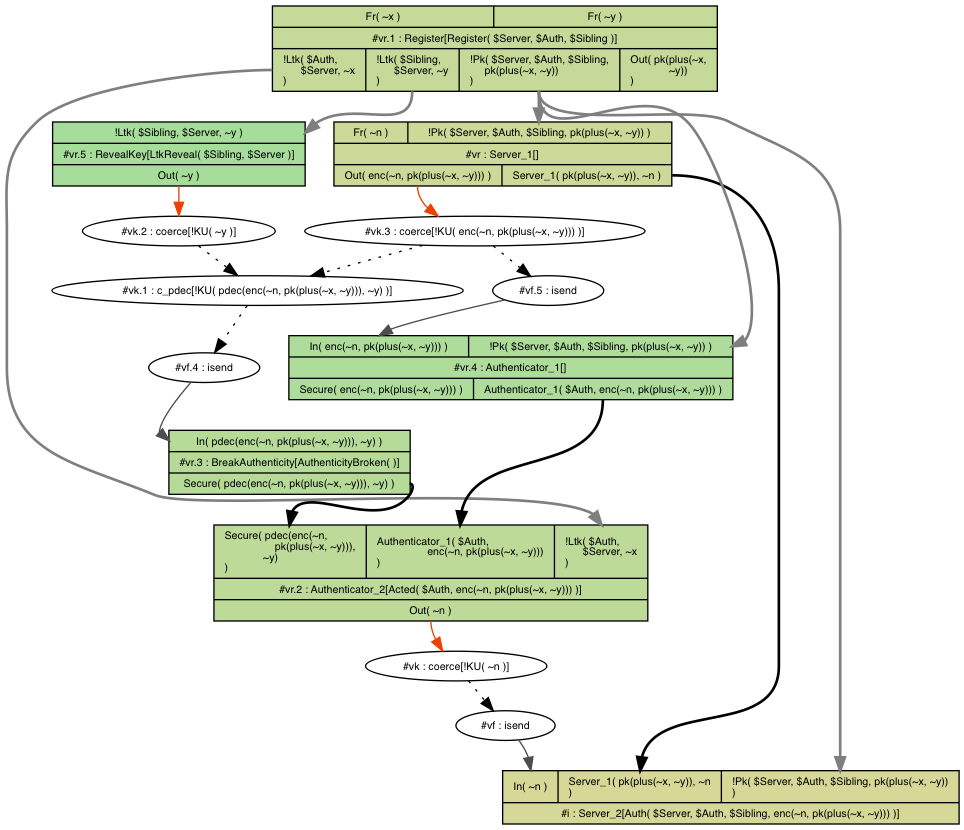
\includegraphics[width=\linewidth]{gfx/attack}
    \end{wide}
    \caption[Tamarin trace of SIO attack]{The tamarin trace of the Strong Internal Observation Attack}
    \label{fig:my_label}
\end{figure}
%********************************************************************
% Other Stuff in the Back
%*******************************************************
%\cleardoublepage%*******************************************************
% Declaration
%*******************************************************
\refstepcounter{dummy}
\pdfbookmark[0]{Declaration}{declaration}
\chapter*{Declaration}
\thispagestyle{empty}
Put your declaration here.
\bigskip
 
\noindent\textit{\myLocation, \myTime}

\smallskip

\begin{flushright}
    \begin{tabular}{m{5cm}}
        \\ \hline
        \centering\myName \\
    \end{tabular}
\end{flushright}

\cleardoublepage\pagestyle{empty}

\hfill

\vfill



%\pdfbookmark[0]{Colophon}{colophon}
%\section*{Colophon}

\noindent With this thesis now ending, so does five years of studies. Thanks to all of our fellow students, professors, and to the IT University of Copenhagen. Thanks to everybody that helped us get this far.

\bigskip

\begin{flushright}{\slshape    
    We have seen that computer programming is an art, \\ 
    because it applies accumulated knowledge to the world, \\ 
    because it requires skill and ingenuity, and especially \\
    because it produces objects of beauty.} \\ \medskip
    --- Donald E. Knuth
\end{flushright}

\bigskip

\noindent\finalVersionString





% ********************************************************************
% Game Over: Restore, Restart, or Quit?
%*******************************************************
\end{document}
% ********************************************************************